\documentclass[12pt]{report}
\usepackage[dvipsnames,svgnames,x11names,hyperref]{xcolor}
\usepackage{fullpage}
\usepackage{amsthm}
\usepackage{amsmath}
\usepackage{amssymb}
\usepackage[colorlinks]{hyperref}
\usepackage[Bjornstrup]{fncychap}
\usepackage{lipsum}
\usepackage{palatino}
\usepackage{todonotes}
\usepackage{mdframed}
\usepackage{tikz}
\usepackage{epigraph}
\usepackage{verbatim}
\usepackage{thmtools}
\usepackage{ccicons}

%%%%%%%%%%%%%%%%%%%%%%%%%%%%%%
%%%%%% Git version info %%%%%%
%%%%%%%%%%%%%%%%%%%%%%%%%%%%%%
\newcommand{\currentversion}{1.3.2}

%%% Local Variables: 
%%% mode: latex
%%% TeX-master: "main"
%%% End: 


% \hypersetup{
%   citecolor={blue}
% }


\usetikzlibrary{arrows}

\numberwithin{equation}{chapter}
\declaretheoremstyle[bodyfont=\it,qed=\qedsymbol]{noproofstyle} 

\declaretheorem[numberlike=equation]{axiom}

\declaretheorem[numberlike=equation]{observation}
\declaretheorem[numberlike=equation,style=noproofstyle,name=Observation]{observationwp}
\declaretheorem[name=Observation,numbered=no]{observation*}

\declaretheorem[numberlike=equation]{fact}
\declaretheorem[numberlike=equation]{subclaim}
\declaretheorem[numberlike=equation]{problem}

\declaretheorem[numberlike=equation]{theorem}
\declaretheorem[numberlike=equation,style=noproofstyle,name=Theorem]{theoremwp}
\declaretheorem[name=Theorem,numbered=no]{theorem*}

\declaretheorem[numberlike=equation]{lemma}
\declaretheorem[name=Lemma,numbered=no]{lemma*}
\declaretheorem[numberlike=equation,style=noproofstyle,name=Lemma]{lemmawp}

\declaretheorem[numberlike=equation]{corollary}
\declaretheorem[name=Corollary,numbered=no]{corollary*}
\declaretheorem[numberlike=equation,style=noproofstyle,name=Corollary]{corollarywp}

\declaretheorem[numberlike=equation]{proposition}
\declaretheorem[name=Proposition,numbered=no]{proposition*}
\declaretheorem[numberlike=equation,style=noproofstyle,name=Proposition]{propositionwp}

\declaretheorem[numberlike=equation]{claim}
\declaretheorem[name=Claim,numbered=no]{claim*}
\declaretheorem[numberlike=equation,style=noproofstyle,name=Claim]{claimwp}

\declaretheorem[numberlike=equation]{conjecture}
\declaretheorem[name=Conjecture,numbered=no]{conjecture*}

\declaretheorem[numberlike=equation]{question}
\declaretheorem[name=Question,numbered=no]{question*}
\declaretheoremstyle[
    headfont=\bfseries, 
    notebraces={[}{]},
    bodyfont=\normalfont\itshape,
    headpunct={},
%    postheadspace=\newline,
%    postheadhook={\textcolor{red}{\rule[.6ex]{\linewidth}{0.4pt}}\\},
    spacebelow=\parsep,
    spaceabove=\parsep,
    mdframed={
        backgroundcolor=white, 
            linecolor=black!80, 
            innertopmargin=6pt,
            roundcorner=5pt, 
            innerbottommargin=6pt, 
            skipabove=\parsep, 
            skipbelow=\parsep } 
]{exercisestyle}

\declaretheorem[name=Open Problem]{openproblem}
\declaretheorem[name=Exercise,style=exercisestyle]{exercise}
\numberwithin{openproblem}{chapter}
\numberwithin{exercise}{chapter}

\declaretheoremstyle[bodyfont=\it,qed=$\lozenge$]{defstyle} 

\declaretheorem[numberlike=equation,style=defstyle]{definition}
\declaretheorem[unnumbered,name=Definition,style=defstyle]{definition*}

\declaretheorem[numberlike=equation,style=defstyle]{example}
\declaretheorem[unnumbered,name=Example,style=defstyle]{example*}

\declaretheorem[numberlike=equation,style=defstyle]{notation}
\declaretheorem[unnumbered,name=Notation=defstyle]{notation*}

\declaretheorem[numberlike=equation,style=defstyle]{construction}
\declaretheorem[unnumbered,name=Construction,style=defstyle]{construction*}

\declaretheorem[numberlike=equation,style=defstyle]{remark}
\declaretheorem[unnumbered,name=Remark,style=defstyle]{remark*}

\renewcommand{\subsectionautorefname}{Subsection}
\renewcommand{\sectionautorefname}{Section}

\newenvironment{myproof}[1]%
{\vspace{1ex}\noindent{\em Proof.}\hspace{0.5em}\def\myproof@name{#1}}%
{\hfill{\tiny \qed\ (\myproof@name)}\vspace{1ex}}
\newenvironment{proof-sketch}{\medskip\noindent{\em Sketch of Proof.}\hspace*{1em}}{\qed\bigskip}
\newenvironment{proof-attempt}{\medskip\noindent{\em Proof attempt.}\hspace*{1em}}{\bigskip}
\newenvironment{proofof}[1]{\medskip\noindent\emph{Proof of #1.}\hspace*{1em}}{\qed\bigskip}


\newcommand{\inparen }[1]{\left(#1\right)}             %\inparen{x+y}  is (x+y)
\newcommand{\inbrace }[1]{\left\{#1\right\}}           %\inbrace{x+y}  is {x+y}
\newcommand{\insquare}[1]{\left[#1\right]}             %\insquar{x+y}  is [x+y]
\newcommand{\inangle }[1]{\left\langle#1\right\rangle} %\inangle{A}    is <A>

\newcommand{\abs}[1]{\left|#1\right|}                  %\abs{x}        is |x|
\newcommand{\norm}[1]{\left\Vert#1\right\Vert}         %\norm{x}       is ||x||

\newcommand{\fspan}[1]{\F\text{-span}\inbrace{#1}}

\newcommand{\union}{\cup}
\newcommand{\Union}{\bigcup}
\newcommand{\intersection}{\cap}
\newcommand{\Intersection}{\bigcap}

\newcommand{\ceil}[1]{\lceil #1 \rceil}
\newcommand{\floor}[1]{\lfloor #1 \rfloor}


\newcommand{\eqdef}{\stackrel{\text{def}}{=}}
\newcommand{\setdef}[2]{\inbrace{{#1}\ : \ {#2}}}      % E.g: \setdef{x}{f(x) = 0}
\newcommand{\set}[1]{\inbrace{#1}}
\newcommand{\innerproduct}[2]{\left\langle{#1},{#2}\right\rangle} %\innerproduct{x}{y} is <x,y>.
\newcommand{\zo}{\inbrace{0,1}}                        % Well just something that is used often!
\newcommand{\parderiv}[2]{\frac{\partial #1}{\partial #2}}
\newcommand{\pderiv}[2]{\partial_{#2}\inparen{#1}}
\newcommand{\zof}[2]{\inbrace{0,1}^{#1}\longrightarrow \inbrace{0,1}^{#2}}


% Commonly used blackboard letters
\newcommand{\FF}{\mathbb{F}}
\newcommand{\F}{\mathbb{F}}
\newcommand{\N}{\mathbb{N}}
\newcommand{\Q}{\mathbb{Q}}
\newcommand{\Z}{\mathbb{Z}}
\newcommand{\R}{\mathbb{R}}
\newcommand{\C}{\mathbb{C}}
\newcommand{\RR}{\mathbb{R}}
\newcommand{\E}{\mathbb{E}}


\newcommand{\zigzag}{\textcircled{z}}  % for the zig-zag product
\newcommand{\poly}{\mathrm{poly}}
\newcommand{\rank}{\mathrm{rank}}


% \newcommand{\char}{\textrm{char}}
% \newcommand{\rank}{\textrm{rank}}
% \newcommand{\dim}{\textrm{dim}}



%% accented words
\newcommand{\Hastad}{H{\aa}stad }
\newcommand{\Godel}{G\"{o}del }
\newcommand{\Mobius}{M\"{o}bius }
\newcommand{\Gauss}{Gau{\ss} }
\newcommand{\naive}{na\"{\i}ve }
\newcommand{\Naive}{Na\"{\i}ve }
\newcommand{\grobner}{gr\"{o}bner }
\newcommand{\bezout}{b\'{e}zout}
\newcommand{\Bezout}{B\'{e}zout}



\newcommand{\Det}{\mathsf{Det}}
\newcommand{\Perm}{\mathsf{Perm}}
\newcommand{\ESym}{\mathrm{Esym}}
\newcommand{\PSym}{\mathrm{Pow}}
\newcommand{\NW}{\mathrm{NW}}
\newcommand{\IMM}{\mathrm{IMM}}


%% Bold letters
\newcommand{\veca}{\mathbf{a}}
\newcommand{\vecb}{\mathbf{b}}
\newcommand{\vecc}{\mathbf{c}}
\newcommand{\vecd}{\mathbf{d}}
\newcommand{\vece}{\mathbf{e}}
\newcommand{\vecf}{\mathbf{f}}
\newcommand{\vecg}{\mathbf{g}}
\newcommand{\vech}{\mathbf{h}}
\newcommand{\veci}{\mathbf{i}}
\newcommand{\vecj}{\mathbf{j}}
\newcommand{\veck}{\mathbf{k}}
\newcommand{\vecl}{\mathbf{l}}
\newcommand{\vecm}{\mathbf{m}}
\newcommand{\vecn}{\mathbf{n}}
\newcommand{\veco}{\mathbf{o}}
\newcommand{\vecp}{\mathbf{p}}
\newcommand{\vecq}{\mathbf{q}}
\newcommand{\vecr}{\mathbf{r}}
\newcommand{\vecs}{\mathbf{s}}
\newcommand{\vect}{\mathbf{t}}
\newcommand{\vecu}{\mathbf{u}}
\newcommand{\vecv}{\mathbf{v}}
\newcommand{\vecw}{\mathbf{w}}
\newcommand{\vecx}{\mathbf{x}}
\newcommand{\vecy}{\mathbf{y}}
\newcommand{\vecz}{\mathbf{z}}

\newcommand{\spaced}[1]{\quad #1 \quad}


%%% Circuit classes
\newcommand{\SPS}{\Sigma\Pi\Sigma}
\newcommand{\SPSP}{\Sigma\Pi\Sigma\Pi}
\newcommand{\SPSE}{\Sigma\Pi\Sigma\wedge}
\newcommand{\SPSPfanin}[2]{\Sigma\Pi^{[#1]}\Sigma\Pi^{[#2]}}
\newcommand{\SPSPsupp}[1]{\Sigma\Pi\Sigma\Pi^{\{#1\}}}
\newcommand{\SESES}{\Sigma\!\wedge\!\Sigma\!\wedge\!\Sigma}

%%% Some complexity classes. (Don't want to include complexity.sty jsut for this. Messes up with \R etc.
\newcommand{\VP}{\mathsf{VP}}
\newcommand{\VNP}{\mathsf{VNP}}
\newcommand{\NP}{\mathsf{NP}}
\newcommand{\BPP}{\mathsf{BPP}}
\renewcommand{\P}{\mathsf{P}}


\newcommand{\FM}{\mathrm{FM}}
\newcommand{\Mon}{\mathrm{Mon}}
\newcommand{\CM}[1]{\Gamma^{\mathrm{[#1]}}}
\newcommand{\SPD}[3]{\inangle{\partial^{=#1}\inparen{#3}}_{\leq #2}}
\newcommand{\mySPSP}[2]{\Sigma\Pi^{[#1]}\Sigma\Pi^{[#2]}}

\renewcommand{\epsilon}{\varepsilon}

%% Some title page jazz. Hat-tip: http://tex.stackexchange.com/questions/85904/showcase-of-beautiful-title-page-done-in-tex
\renewcommand\epigraphflush{flushright}
\renewcommand\epigraphsize{\normalsize}
\setlength\epigraphwidth{0.7\textwidth}

\definecolor{titlepagecolor}{cmyk}{1,.60,0,.40}

\DeclareFixedFont{\titlefont}{T1}{ppl}{b}{it}{0.5in}

\makeatletter                       
\def\printauthor{%                  
    {\large \@author}}              
\makeatother
\author{%
    Ramprasad Saptharishi \\
    Tel Aviv University \\
    \texttt{ramprasad@cmi.ac.in}
    }


\begin{document}

\begin{titlepage}
\noindent
\vspace*{1cm}

\titlefont A survey of known lower\par bounds for arithmetic \par circuits\par
\epigraph{\tt https://github.com/dasarpmar/lowerbounds-survey}{Version \currentversion}
\null\vfill
\vspace*{1cm}
\noindent
\hfill
\begin{minipage}{0.50\linewidth}
    \begin{flushright}
      {\Large {\bf Contributing authors:}}

      \vspace*{1cm}

        \printauthor
    \end{flushright}
\end{minipage}
%
\begin{minipage}{0.02\linewidth}
    \rule{1pt}{125pt}
\end{minipage}
\end{titlepage}


\chapter*{Preface}

Arithmetic circuit complexity has seen a flurry of activity recently with respect to lower bounds. There suddenly seems to be some optimism proving explicit circuit lower bounds in the near future. Besides the question of lower bounds, there has also been tremendous progress on polynomial identity testing and polynomial reconstruction as well. 

In 2014, I was a part of two surveys on arithmetic circuit lower bounds. The first one \cite{KayalRP} was with Neeraj Kayal, and was a  part of a volume dedicated to Somenath Biswas' 60th Birthday Celebrations. This survey was a comprehensive article of almost all known lower bound proofs at that time. Soon after the survey was written, there were more lower bounds proved for homogeneous depth four circuits. The second survey \cite{rp:beatcs} appeared in the Bulletin of the EATCS and this focused on those lower bounds for homogeneous depth four circuits (among some other results). 

Instead of writing a new survey every time there are a fresh set of lower bounds, a better idea was to have one expanding survey that is kept up to date with the current state of the art. Much like an application, that keeps getting updated and new releases. Also, this would be greatly accelerated if the community could contribute by looking for bugs, adding more content, changing presentation etc. The natural answer to all this was to do this the way software applications are built, and I chose github as that is the most popular platform for this. \\

\noindent 
This survey would be present on:
\begin{quote} 
  \url{https://github.com/dasarpmar/lowerbounds-survey}
\end{quote}
and anyone is welcome to contribute to it. The github repository also has a wiki to assist people who are new to git and/or github. \\



\subsection*{What to expect from this article}

Most of the proofs in this article are complete and self-contained. However, as one would expect in the more delicate proofs, there would eventually involve a fair amount of calculation and setting of parameters. There might be proofs where this last technical calculation is avoided, but the hope is to make the presentation insightful enough so that it would enable any student to do the calculations (him/her)self.

Also, quite a lot of the proofs presented here are slightly different from the original proofs. The reason for the deviation would almost always be for more clarify and intuition. However, this process might also make the parameters involved a little weaker than in the original statements. We shall try to ensure that such losses do not change the overall strength of the theorem by much, and if they do we shall mention that explicitly. \\

\subsection*{Why do we need this?}

\begin{quote}
So why are super polynomial lower bounds still not proved?  Maybe it's because not enough people are working on it.  
\begin{flushright}
-- Ran Raz (in \cite{raz10fool})
\end{flushright}
\end{quote}


I strongly believe that the above statement really hits the nail on the head. Fortunately, over the last few years we have seen such a phenomenal activity in arithmetic circuit lower bounds and an increased optimism that we can indeed soon prove super-polynomial circuit lower bounds. In fact, a lot of the recent lower bounds have come really close to this goal. The hope of this survey is that this would assist people familiarize with the known lower bounds and develop the necessary tools. As a student, the surveys of \cite{sy,ckw11} were immensely helpful and this is an attempt to give back to the community. 

\vspace*{2cm}

\noindent
Ramprasad Saptharishi

\noindent
27th November 2014

\noindent 
Version \currentversion

%%% Local Variables: 
%%% mode: latex
%%% TeX-master: "main"
%%% End: 


\chapter*{Contributors to this article}

\section*{Content}

\begin{itemize}
\item Ramprasad Saptharishi (Tel Aviv University)

\texttt{ramprasad@cmi.ac.in}
\end{itemize}

\section*{Corrections, minor edits}

\begin{itemize}
\item V Vinay (Limberlink Technologies)

\texttt{vinay@jed-i.in}
\end{itemize}


%%% Local Variables: 
%%% mode: latex
%%% TeX-master: "main"
%%% End: 


\hypersetup{
  linkcolor={DarkSlateGray}
}
\tableofcontents
\hypersetup{
  linkcolor={red}
}

\part{Preliminaries}

\chapter{Introduction}\label{chap:intro}


``What is the best way to compute a given polynomial $f(x_1,\dots, x_n)$ from basic operations such as $+$ and $\times$?'' This is the main motivating problem in the field of arithmetic circuit complexity. 
The notion of \emph{complexity} of a polynomial is measured via the size of the smallest arithmetic circuit computing it. 
Arithmetic circuits provide a robust model of computation for polynomials. 
Formally, these are directed acyclic graphs with a unique sink vertex, where internal nodes are labelled by $+$ and $\times$ and each source node labelled with either a variable or a field constant. 
Each $+$ gate computes the sum of the polynomials computed at its children, and $\times$ gates the product. 
The unique sink vertex is called the root or the output gate, and the polynomial computed by that gate is the polynomial computed by the circuit. 

There are several interesting questions that can be asked about arithmetic circuits, and polynomials that they compute. 
One category of problems are of the form, ``Is there an explicit polynomial $f(x_1,\dots, x_n)$ that require (perhaps restricted) arithmetic circuits of size $2^{\Omega(n)}$ to compute them?'', or questions about proving lower bounds. 
Another category of problems are of the form, ``Is the given circuit computing the $0$ polynomial?'', which is also called `Polynomial Identity Testing (PIT)'. 
Yet another class of questions are of the form ``Given oracle access to a circuit, can you write down the polynomial computed by this circuit?'', which are also called `polynomial reconstruction'. 
Several of these problems have very strong connections between each other despite being of very different flavours. 
Formal connections between PIT and lower bounds have been shown by \cite{ki03,a05}. 
Further, strong lower bounds for restricted models have often been succeeded by reconstruction algorithms (at least on average). 
In this article we shall mainly be looking at lower bounds. 
For more on reconstruction and PIT questions, the author is invited to read other excellent surveys such as \cite{sy,ckw11}. 

\section{Arithmetic complexity classes}
In the seminal paper of \cite{v79}, Valiant defined two classes of polynomials which we now call $\VP$ and $\VNP$. 

\begin{definition}
The class $\VP$ is defined as the set of all polynomial $f(x_1,\dots, x_n)$ with $\deg(f) = n^{O(1)}$ that can be computed by an arithmetic circuit of size $s = n^{O(1)}$. 

The class $\VNP$ is defined as the set of all polynomial $f(x_1,\dots, x_n)$ such that there exists a $g(x_1,\dots, x_n, y_1,\dots, y_m)$ with $m = n^{O(1)}$ such that
\[
f(x_1,\dots, x_n) \quad = \quad \sum_{y_1=0}^1\dots \sum_{y_m=0}^1 g(x_1,\dots, x_n, y_1,\dots, y_m)
\]
\end{definition}
The class $\VP$ is synonymous to what we understand as \emph{efficiently computable} polynomials. 
The class $\VNP$, whose definition is similar to the boolean class $\NP$, is in some sense a notion of what deem as \emph{explicit}. 

\begin{fact}
Let $f(x_1,\dots, x_n)$ be a polynomial such that $\deg(f) = n^{O(1)}$ and given any exponent vector $e_1,\dots, e_n$, the coefficient of the monomial $x_1^{e_1}\dots x_n^{e_n}$ in $f$ can be computed in polynomial time. 
Then, $f \in \VNP$. 
\end{fact}

For example, consider the permanent of a symbolic $n\times n$ matrix. 
In fact, \cite{v79} showed that the symbolic $n\times n$ permanent is in some sense complete for the class $\VNP$. 
Further, he also showed that the determinant of a symbolic  $n\times n$ matrix is (almost) complete for the class $\VP$. 
Separating the determinant and the permanent is the Holy Grail in the field of arithmetic circuit complexity. \\

{\bf Remark.} Note that the above fact merely gives a sufficient condition for a polynomial to be in $\VNP$. 
There are examples of polynomials $f$ where computing the coefficient of a given monomial is believed to be very hard but $f\in \VNP$.\footnote{For example, consider the $n^2$ variate multilinear polynomial $f$ such that the coefficient $x_{11}^{e_{11}}\dots x_{nn}^{e_{nn}}$ is the permanent of the $n\times n$ matrix $(\!(e_{ij})\!)_{i,j}$. 
Turns out $f \in \VNP$. 
In fact, a necessary and sufficient condition is that the coefficient of a given monomial can be computed in $\#\mathsf{P}/\poly$. }  In this article however, all the polynomials we shall be dealing with would have this property that the coefficient of a given monomial can be efficiently computed. 
For more about completeness classes in arithmetic complexity, \cite{bcs97} is a wonderful text. 


\section{Prior lower bounds}

Proving lower bounds is generally considered challenging, in most models of computation. 
For general circuits, the best lower bound we have for an explicit polynomial is by \cite{BS83} who prove an $\Omega(n\log n)$ lower bound. 
For the subclass of arithmetic formulas, \cite{k85} has shown a $\Omega(n^{3/2})$ lower bound. 
On the other hand, we know by standard counting methods that most $n$-variate degree $d$ polynomials require circuits of size $\Omega\inparen{\sqrt{\binom{n+d}{d}}}$.

To gain better understanding of computation by arithmetic circuits, researchers focused on proving lower bounds for restricted models of computation. 
One very natural restriction is the depth of the circuit. 
Proving lower bounds for depth two circuits are trivial. 
For general depth three circuits, the best lower bound we have is by \cite{sw2001} who present an $\Omega(n^2)$ lower bound. 
Exponential lower bounds are known with additional restrictions like \emph{homogeneity} \cite{nw1997}, \emph{multilinearity} \cite{raz2004,raz-yehudayoff}, over finite fields \cite{gr00,grigoriev98}, \emph{monotonicity} \cite{js82} etc. 

For multilinear models, more is known for even larger depth. \cite{raz2004} showed an $n^{\Omega(\log n)}$ lower bound for the class of multilinear formulas. \cite{raz-yehudayoff} extended those techniques to show an $2^{n^{\Omega(1/\Delta)}}$ lower bound for multilinear formulas of depth $\Delta$. 

\section{Relevance of shallow circuits for ``$\VP$ vs $\VNP$''}

The study of lower bounds for shallow circuits is not just an attempt to simplify the problem and gain insight on the larger goal. 
The class of shallow arithmetic circuits are surprisingly powerful, unlike the boolean case. 
Shallow circuits in the arithmetic world almost capture the entire computational power of unrestricted circuits! 

There has been a long series of results that simulate a general arithmetic circuit $C$ by a \emph{shallow} circuit of size comparable to the size of $C$. 
This task simulating a circuit but another not-too-large circuit of small depth is called \emph{depth reduction}. 
The first result in this regard is by \cite{vsbr83} who proved the following. 

\begin{theorem}[\cite{vsbr83}]
Let $f$ be an $n$-variate degree $d$ polynomial computed by an arithmetic circuit $C$ of size $s$. 
Then, $f$ can be equivalently computed by a homogeneous circuit $C'$ of depth $O(\log d)$ with unbounded fan-in $+$ and $\times$ gates and size $s' = (nds)^{O(1)}$. 
\end{theorem}


The above theorem allows us to focus on just homogeneous circuits of $O(\log d)$ depth and attempt lower bounds for this model. 
Any super-polynomial lower bound for the class of $O(\log d)$ depth circuits automatically yields a super-polynomial lower bound for general circuits. \\

However, if we really hope to prove much stronger lower bounds for $\Perm_n$ like say $2^{\Omega(n)}$, maybe we can afford to incur a slightly larger blow-up in size to obtain an even shallower circuit. 
This line was first pursued by \cite{av08}, and subsequently strengthened by \cite{koiran} and \cite{Tav13} to yield the following result. 

\begin{theorem}[\cite{av08,koiran,Tav13}] 
  Let $f$ be an $n$-variate degree $d$ polynomial computed by an arithmetic circuit of size $s$. 
Then $f$ can be computed by a homogeneous $\SPSPfanin{O(\sqrt{d})}{\sqrt{d}}$ circuit of size $s' \leq s^{O(\sqrt{d})}$

More generally, for any $0\leq r\leq d$, there is a homogeneous $\SPSPfanin{O(d/r)}{r}$ circuit of top fan-in at most $s^{O(d/t)}$ computing $f$. 
\end{theorem}

Recall that a $\SPSPfanin{O(\sqrt{d})}{\sqrt{d}}$ circuit computes a polynomial of the form
\[
f\spaced{=} \sum_{i=1}^s Q_{i1}\dots Q_{ia} \quad,\quad \text{where $a = O(\sqrt{d})$ and $\deg Q_{ij} \leq \sqrt{d}$}
\]

In other words, if we can prove a lower bound of $n^{\omega(\sqrt{d})}$ for the class of $\SPSPfanin{O(\sqrt{d})}{\sqrt{d}}$ circuits, we would have a super-polynomial lower bound for the class of general arithmetic circuits! 
In fact, the model of depth $4$ circuits seem so central in that almost all known lower bounds for other restricted models proceed by proving a suitable lower bound for a depth $4$ analogue. 
Several examples of this may be seen in \cite{KayalRP}. \\

The first breakthrough was obtained by \cite{gkks13} who showed an $2^{\Omega(\sqrt{d})}$ lower bound for such circuits computing the symbolic $d\times d$ determinant or permanent. 
Subsequently, there was a flurry of activity towards achieving the goal of proving $n^{\omega(\sqrt{d})}$ lower bounds \cite{KSS13,FLMS13,KS14a}, and this is where we currently stand. 

\begin{theorem}
There is an explicit homogeneous $n$-variate degree $d$ polynomial $f$ that can be computed by a homogeneous depth $4$ circuit of size $n^{O(1)}$ but any $\SPSPfanin{O(\sqrt{d})}{\sqrt{d}}$ computing it requires top fanin $s = n^{\Omega(\sqrt{d})}$.
\end{theorem}

If we could change the $n^{\Omega(\sqrt{d})}$ to $n^{\omega(\sqrt{d})}$ in the above theorem (of course, the polynomial $f$ cannot then have a small arithmetic circuit computing it), we would have proved a super-polynomial lower bound for general arithmetic circuits! 
The following is the simplest formulation of a lower bound of shallow circuit that would imply lower bounds for general circuits. \\

\begin{openproblem}\label{openprob:main} Find an explicit $n$-variate degree $d$ polynomial $f$ such that any expression of the form
\[
f \quad=\quad (Q_1)^{\sqrt{d}} + \dots + (Q_{s})^{\sqrt{d}}\quad,\quad \deg(Q_i) \leq \sqrt{d} \text{ for all $i$}
\]
must have $s = n^{\omega(\sqrt{d})}$. 
\end{openproblem}
\bigskip 

Subsequent to this line of work, several researchers addressed the task of proving lower bounds for homogeneous depth $4$ circuits without any restriction on the fan-ins. 
It is worth noting that a lower bound for homogeneous depth $4$ circuits must be on the total size and not the top fan-in, as otherwise one could just compute the polynomial $f$ in a single gate of the bottom two layers. 

\subsection*{What to expect from this article}

This article is intended to be a rolling survey of (almost) all known lower bounds in arithmetic circuit complexity. 
Most of the proofs in this article are complete and self-contained. 
However, as one would expect in the more delicate proofs, there would eventually involve a fair amount of calculation and setting of parameters. 
There might be proofs where this last technical calculation is avoided, but the hope is to make the presentation insightful enough so that it would enable any student to do the calculations (him/her)self.

Also, quite a lot of the proofs presented here are slightly different from the original proofs. 
The reason for the deviation would almost always be for more clarify and intuition. 
However, this process might also make the parameters involved a little weaker than in the original statements. 
We shall try to ensure that such losses do not change the overall strength of the theorem by much, and if they do we shall mention that explicitly. 

\subsection*{What is not (yet) covered in this survey}

There are surely a few notable lower bounds that are not (yet) discussed in the survey.
A few that come to mind are the super-linear lower bound of Raz, Shpilka and Yehudayoff for syntactic multilinear circuits \cite{RSY08} and some more recent lower bounds involving shifted partial derivatives that are yet to be included. 

Besides lower bounds, there are many approaches to prove lower bounds such as Raz's lower bound approach via elusive functions \cite{Raz10elusive}, or Valiant's rigidity approach, or the sum-of-squares question of \cite{hwy}, or the Real $\tau$ conjecture, Geometric Complexity Theory etc.

Perhaps some of these gaps shall be filled in the near\footnote{:-)} future.
Perhaps.

%%% Local Variables: 
%%% mode: latex
%%% TeX-master: "fancymain"
%%% End: 


\chapter{Notation and Preliminaries}\label{chap:notation}

We first explain some notation that shall be used throughout this article. 

\begin{itemize}
\item In most cases, the degree of the polynomial shall be denoted by $d$ and the number of variables shall be denoted by $n$. 
In some cases, $n$ would refer to a parameter that would determine the number of variables (though perhaps not exactly). 
\item Almost all the polynomials that we shall be studying would be multilinear. 
In multilinear polynomials, we shall identify a monomial with the \emph{set of variables} that it is a product of. 
This would allow us to abuse notation and say $x_i \in m$ to mean that $x_i$ divides the monomial $m$, or to say $m_1 \intersection m_2$ to refer to the $\gcd(m_1,m_2)$. 
We shall also use the notation $m \in f$ to mean that the polynomial $m$ has a non-zero coefficient for the monomial $m$. 
\item We shall use $[n]$ to denote $\inbrace{1,\dots, n}$ and we shall use boldface letters such as $\mathbf{x}$ to denote sets of variables. 
Further, $\mathbf{x}_{[n]}$ shall refer to a set of variables $\inbrace{x_1,\dots, x_n}$. 
However, if the number of variables is understood, we shall drop the subscript. 
\end{itemize}


\section{Models of computation}

As mentioned earlier, the most robust model of computation that are studied are arithmetic circuits, which are formally defined as follows. 

\begin{definition}[Arithmetic circuits and formulas]\label{defn:arithmetic-circuit}
An arithmetic circuit is a directed acyclic graph with a unique sink vertex called the \emph{root}. 
The source vertices are labelled by either formal variables or field constants, and each internal node of the graph is labelled by either $+$ or $\times$. 
Nodes compute formal polynomials in the input variables  in the natural way. 
Further, edges entering a $+$ nodes also might have field constants on them to allow the $+$ to compute an $\F$-linear combination of the children (rather than just a sum). 

The polynomial computed by the circuit is defined as the polynomial computed by the root. \\

\noindent
If the underlying graph is a \emph{tree} instead of a general acyclic graph, the circuit is called a \emph{formula}.
\end{definition}


Another model of computation that is studied often is the model \emph{algebraic branching programs}, defined as follows. 

\begin{definition}[Algebraic Branching Program]\label{defn:ABP}
An algebraic branching program (ABP) is a layered graph with a unique source vertex (that we shall call $s$) and a unique sink vertex (that we shall call $t$). 
All edges are from layer $i$ to layer $i+1$, and each edge is labelled by a linear polynomial. 
The polynomial computed by the ABP is defined as 
\[
f\spaced{=} \sum_{\gamma: s \leadsto t} \mathrm{wt}(\gamma)
\]
where for every path $\gamma$ from $s\leadsto t$, the weight $\mathrm{wt}(\gamma)$ is defined as the product of the labels over the edges in $\gamma$. 
\end{definition}

The width of the ABP is defined as the maximum number of vertices in any layer, and the depth is defined as the length of the longest path from $s$ to $t$. 
The polynomial computed by an ABP is captured by the \emph{iterated matrix multiplication} polynomial that we shall soon see. 

It is easy to observe that any arithmetic formula of size $s$ can be simulated by an algebraic branching program of size $\poly(s)$, and any algebraic branching program of size $s$ can be simulated of an arithmetic circuit of size $\poly(s)$. 
It is a major open problem to show a separation between any of these. 

\[
\mathrm{Formulas} \spaced{\subseteq} \mathrm{ABPs} \spaced{\subseteq} \mathrm{Circuits}
\]

\begin{openproblem}
Show a super-polynomial separation between any of the models -- formulas, ABPs and circuits. 
\end{openproblem}

\subsection{Constant depth circuits}

We shall be dealing a lot with constant depth circuits. 
Normally, the root is assumed to be a $+$ gate\footnote{the reason for this is that often the polynomial computed by the circuits would be irreducible, and hence would be silly to have a $\times$ gate as a root.} and the circuit is assumed to consist of alternating layers of $+$ and $\times$ gates. 
A layer of $+$ gates are called $\Sigma$ layers, and a layer of $\times$ gates are called $\Pi$ layers. 
Thus, a depth two circuit consist of the form 
\[
f\quad = \quad \sum_{i=1}^s \prod_{j=1}^d x_{ij}
\]
is a $\Sigma\Pi$ circuit. 

\begin{fact}
Any arithmetic circuit of depth $\Delta$ and size $s$, can be simulated by an arithmetic formula of depth $\Delta$ and size $s' \leq s^{\Delta}$. 
\end{fact}

Thus for constant depth circuits (where $\Delta = O(1)$), we may assume that we are dealing with formulas without much loss of generality.


It would also be useful to keep track of the \emph{fan-in} of the gates in a certain layer (especially of multiplication gates). 
We shall use superscripts to denote this. 
For example, an $\Sigma\Pi^{[a]}\Sigma\Pi^{[b]}$ circuits computes a polynomial of the form
\[
f \spaced{=} \sum_i \prod_{j=1}^a Q_{ij}
\]
where each $Q_{ij}$ is a polynomial of degree at most $b$. \\

It would also be useful to consider special layers of multiplication gates that multiply the same polynomial several times, rather than multiplying several different polynomials together. 
Since such gates simply raise the input to a certain power, these would be called \emph{exponentiation} gates. 
A layer of exponentiation will be denoted by $\wedge$ \footnote{To say a little on the choice of notation, it was introduced in \cite{gkks13b} and the first choice was to use ${}^{\wedge}$, but looked rather ugly to write it as say $\Sigma{}^{\wedge}\Sigma$. 
Hence, $\Sigma\!\wedge\!\Sigma$  was chosen instead. } and, for example, a $\Sigma\!\wedge\!\Sigma$ circuit computes a polynomial of the form 
\[
f\spaced{=} \sum_{i=1}^s \ell_{i}^d
\]
where each $\ell_i$ is a linear polynomial. \\

\begin{exercise}
Show that any constant width ABP can be simulated by a polynomial sized formula. 
\end{exercise}



\section{Polynomials of interest}

There are a few polynomials that are the usual suspects while proving lower bounds. 
The polynomials that we would be dealing with in this article are defined below. 

\subsection*{The determinant and the permanent families}

The determinant of an $n\times n$ symbolic matrix shall be denoted by $\Det_n$ and is defined as
\[
\Det_n \spaced{=} \sum_{\sigma \in S_n} \text{sign}(\sigma) x_{1,\sigma(1)}\dots x_{n,\sigma(n)}
\]
The permanent of an $n\times n$ symbolic matrix shall be denoted by $\Perm_n$ and is defined as
\[
\Perm_n \spaced{=} \sum_{\sigma \in S_n}x_{1,\sigma(1)}\dots x_{n,\sigma(n)}
\]

Both of these polynomials are of degree $n$ and over $n^2$ variables. 
We know that $\Det_n$ can be computed by a polynomial sized arithmetic circuit and it is widely believed that the permanent requires circuits of size $2^{\Omega(n)}$. 

\subsection*{The Nisan-Wigderson polynomial families}

Let $n,m,d$ be arbitrary parameters with $m$ being a power of a prime, and $n,d\leq m$. 
Since $m$ is a power of a prime, let us identify the set $[m]$ with the field $\F_m$ of $m$ elements. 
Note that since $n \leq m$, we have that $[n] \subseteq \F_m$. 
The Nisan-Wigderson polynomial with parameters $n,m,d$, denoted by $\mathrm{NW}_{n,m,d}$ is defined as
\[
\NW_{n,m,d}(\vecx) \spaced{=} \sum_{\substack{p(t) \in \F_m[t]\\ \deg(p) \leq d}} x_{1,p(1)}\dots x_{n,p(n)}
\]
That is, for every univariate polynomial $p(t) \in \F_m[t]$ of degree at most $d$, we add one monomials that encodes the `graph' of $p$ on the points $[n]$. 
This is a polynomial of degree $n$ over $mn$ variables.

This monomials of this polynomial satisfy a very useful ``low pairwise-intersection'' property. 

\begin{lemma}\label{lem:NW-low-intersection}
Let $m_1$ and $m_2$ be any two distinct monomials in $\NW_{n,m,d}(\vecx)$. 
Then, there are at most $d$ variables that divide both $m_1$ and $m_2$. 
\end{lemma}
\begin{proof}
Let $m_1$ and $m_2$ correspond to univariates $p_1(t), p_2(t) \in \F_m[t]$ of degree at most $d$. 
Then if $x_{ij}$ divides $m_1$, then $p_1(i) = j$, similarly for $m_2$. 
But since $p_1$ and $p_2$ are two distinct polynomials of degree at most $d$, they can agree in at most $d$ evaluations. 
Thus, there can be at most $d$ variables that divide both $m_1$ and $m_2$. 
\end{proof}

For most generic choices of the parameters, the polynomial $\NW_{n,m,d}$ is believed to require circuits of exponential size to compute them. 

\subsection*{The Iterated-Matrix-Multiplication polynomial}

For parameters $n$ and $d$, the Iterated-Matrix-Multiplication polynomial, denoted by $\IMM_{n,d}$, is defined as follows
$$
\IMM_{n,d} \spaced{=} \sum_{1\leq i_1,\dots, i_d\leq n} x_{1,i_1}^{(1)}x_{i_1,i_2}^{(2)}\dots x_{i_{d-2},i_{d-1}}^{(d-1)}x_{i_{d-1},1}^{(d)}.
$$
An equivalent way of defining the polynomial as the $(1,1)$-th entry of the product of $d$ generic $n\times n$ matrices:
$$
\IMM_{n,d} \spaced{=} \inparen{\insquare{\begin{array}{ccc} x_{11}^{(1)} & \dots & x_{1n}^{(1)}\\ \vdots & \ddots & \vdots \\ x_{n1}^{(1)} & \dots & x_{nn}^{(1)}\end{array}} \cdots \insquare{\begin{array}{ccc} x_{11}^{(d)} & \dots & x_{1n}^{(d)}\\ \vdots & \ddots & \vdots \\ x_{n1}^{(d)} & \dots & x_{nn}^{(d)}\end{array}}}_{(1,1)}.
$$

It is often useful to think of this as the polynomial computed by a \emph{generic algebraic branching program} of width $n$ and depth $n$ (where the edge connecting vertex $i$ of layer $\ell$ to vertex $j$ of layer $\ell+1$ has weight $x_{ij}^{(\ell)}$). 

This is a polynomial of degree $d$ and over $n^2(d-2) + 2n$ variables\footnote{only the first row of the first matrix, and the first column of the last matrix participates in the $(1,1)$ entry of the product}. 
Further, since the polynomial corresponds to a generic algebraic branching program, $\IMM_{n,d}$ can be computed by an arithmetic circuit of size $\poly(n,d)$. 


%%% Local Variables: 
%%% mode: latex
%%% TeX-master: "main"
%%% End: 

\chapter{Algebraic complexity classes} \label{chap-vpvnp}

Valiant \cite{v79}, in his seminal paper, defined two algebraic complexity classes that can be thought of as analogues of the boolean classes $\P$ and $\NP$. This chapter shall focus on their definitions, and some important properties related to the polynomial families $\Det_n$ and $\Perm_n$. 

\section{Definition of classes}

Recall that $\P$ is\footnote{if one is to be more precise, this is $\P/\poly$ or non-uniform $\P$. But in this article, we shall be interested only in the non-uniform versions since we shall mainly deal with circuit sizes.} the class of boolean functions that can be computed by circuits of polynomial size. Note that any boolean function can be expressed as a multilinear\footnote{a polynomial where the degree in any variable is bounded by $1$} polynomial. An analogue of this in the arithmetic world could be multilinear polynomials $f(x_1,\dots, x_n)$ that can be computed by arithmetic circuits of size $\poly(n)$. However, unlike in the boolean world, the polynomial $x^2$ is not equal to the polynomial $x$ as we are dealing with formal polynomials. Valiant's definition of $\VP$ was the class of the class of ``low degree'' polynomials that can be computed by circuits of small size. 

\begin{definition}[Valiant's $\P$]\label{defn:vp}
The class $\VP$ refers to the set of polynomials $f(x_1,\dots, x_n)$ of \emph{degree $\poly(n)$} that can be computed by arithmetic circuits of size $\poly(n)$. 
\end{definition}

In the literature, one also encounters classes such as $\mathsf{VBP}$ and $\mathsf{VF}$ that correspond to polynomials computed by polynomial-sized ABP and formulas respectively.


\subsection*{More on the low-degree restriction}

Note that if one has an arithmetic circuit consisting of a chain of $s$ multiplication gates, it can compute a polynomial of degree $\mathrm{exp}(s)$ (by repeated squaring). But should the analogue of $\VP$ not be the class of polynomials that are computable by $\poly(n)$-sized arithmetic circuits (that include such polynomials of very large degree)? Let us first take a moment to understand why the additional restriction of ``low-degree'' in the above definition of $\VP$ was imposed. This discussion is from an answer by Joshua Grochow on \texttt{cstheory.SE} \cite{gro:SE}. 

\begin{enumerate}

\item Every boolean function can be expressed as a multilinear polynomial. Multilinear polynomials are of course polynomials of ``low degree''. 

\item Much of the earlier work were based on understanding formula size. In the case of arithmetic formulas, the degree cannot be more than the size of the formula. Hence, if a polynomial is computed by a $\poly(n)$ sized formula, then its degree must be bounded by $\poly(n)$ too. 

\item Most interesting polynomials such as $\Det_n$ or $\Perm_n$ are in fact of low degree. Once we choose to deal with only polynomials of low degree, the above definition does not have any restriction on the circuit used to compute it (besides its size). It is certainly possible that intermediate computations of the circuit could involve very large degree polynomials. 

However, as we shall soon see, Strassen's result shows that such high degree computations may be eliminated with just an $O(\deg^2)$ increase in size. Dealing with low-degree circuits also makes the class robust under this transformation. The same blow-up also holds while eliminating division gates in the circuit. 

\item Without this restriction, cannot hope to show that $\Det_n$ or $\Perm_n$ is ``complete'' for such classes, or the numerous structural results such as depth reduction that we have. 

\end{enumerate}

Having said that, there is also a notion of ``degree'' in a boolean circuit that is defined syntactically as follows:
 \begin{quote}
   Degree of all leaves is $1$. 

   For any OR gate, the degree is the maximum of the degree of its children. 

   For any AND gate, the degree is the sum of the degrees of its children. 
 \end{quote}
The class boolean functions that can be computed by poly-sized poly-degree circuits coincide with a class called $\mathsf{LOGCFL}$ or $\mathsf{SAC}^1$. With this notion, one might say that $\VP$ is really an analogue of $\mathsf{SAC}^1$\\


We now move on to the arithmetic analogue of the class $\NP$. Recall that the class $\NP$ may be defined as the set of all boolean functions $f(x_1,\dots, x_n)$ such that there is some $g(x_1,\dots, x_n, y_1,\dots, y_m)$ with $m = \poly(n)$ such that 
\[
f(x_1,\dots, x_n)\spaced{=} \bigvee_{\veca \in \inbrace{0,1}^m}  g(x_1,\dots, x_n, a_1,\dots, a_m)
\]
Valiant's $\NP$ is defined analogously by replacing the OR by a sum. 

\begin{definition}[Valiant's $\NP$]\label{defn:vnp}
The class $\VNP$ is defined to be the set of polynomials $f(x_1,\dots, x_n)$ such that there is some $g(x_1,\dots, g_n, y_1,\dots, y_m) \in \VP$ with $m = \poly(n)$ such that 
\[
f(x_1,\dots, x_n)\spaced{=} \sum_{\veca \in \inbrace{0,1}^m}  g(x_1,\dots, x_n, a_1,\dots, a_m)
\]
\end{definition}

It follows from definitions that $\mathsf{VF} \subseteq \mathsf{VBP} \subseteq \VP \subseteq \VNP$. It is not clear if any of the above inequalities are strict. 

\section{Some properties of these classes}

We shall state a few properties of these classes here. For a more extensive treatment, B\"{u}rgisser's book \cite{bur00} has a comprehensive study of these classes and a lot of the proofs are based on the description there. \\

Valiant~\cite{v79} presented a very useful sufficient condition to show that a given polynomial is in $\VNP$. 

\begin{theorem}[Valiant's Criterion] \label{thm:val-criterion}
Let $f = \sum_\vece c(\vece) \cdot x_1^{e_1}\dots x_n^{e_n}$. Suppose the function $\varphi$ that takes as input the exponent vector $\vece = (e_1,\dots, e_n)$ and outputs the coefficient $c(\vece)$ is in the class $\#\P/\poly$, then $f \in \VNP$. 
\end{theorem}

Thus in particular, if we compute the coefficient for a given monomial in polynomial time, then the polynomial is in $\VNP$. 

\begin{corollary}
The polynomials $\Perm_n$ and $\NW_{n,m,d}$ are in $\VNP$. 
\end{corollary}

Notice that in Definition~\ref{defn:vnp}, the polynomial $g(x_1,\dots, x_n, y_1,\dots, y_m) \in \VP$. However, a subsequent paper of Valiant showed that we may assume with loss of generality that $g \in \mathsf{VF}$, that is $g$ is computable by a small formula. This is similar to the fact that counting solutions of 3-\textsf{CNF} instance, which is a formula, is as hard as counting solutions of any polynomial sized boolean circuit. We state this result here, and a proof may be found in B\"urgisser's book \cite{bur00}. 

\begin{theorem}\label{thm:vnp-formula}
For any $f(x_1,\dots, x_n)\in \VNP$, there is a $g(x_1,\dots, x_n, y_1,\dots, y_m)$ that can be computed by a $\poly(n)$ sized \emph{formula} such that 
\[
f(x_1,\dots, x_n)\spaced{=} \sum_{\veca \in \inbrace{0,1}^m} g(x_1,\dots, x_n, a_1,\dots, a_m)
\]
\end{theorem}

\section{Reductions and completeness}

For polynomials, the most natural form of reductions are via \emph{projections}. We shall say that a polynomial $f$ \emph{reduces} to $g$ via projections if $g$ may be obtained by setting substituting variables of $f$ to other variables or field constants. Under such reductions, do we have natural complete polynomials for the classes $\VP$ and $\VNP$? Valiant \cite{v79} showed that the $\Det_n$ and $\Perm_n$ are (almost) complete for the classes $\VP$ and $\VNP$ respectively. We shall see the proof of this in this section. 

\begin{theorem}[\cite{v79}]\label{thm:vp}
If $f$ is a polynomial computed by an ABP of size $s$, then $f$ reduces to $\Det_n$ via projections for $n = \poly(s)$. 
\end{theorem}
\begin{theorem}[\cite{v79}]\label{thm:vnp}
Over any field $\F$ of characteristic not equal to $2$, the polynomial $\Perm_n$ is \emph{complete} for the class $\mathsf{VNP}$ under projections.
\end{theorem}

\subsubsection*{Graph theoretic representation of $\Det_n$ and $\Perm_n$}

Let us think of an $n\times n$ symbolic matrix as an adjacency matrix of a directed graph $G$ with the edge from $i$ to $j$ having weight $x_{ij}$. Then every monomial of $\Det_n$ or $\Perm_n$ corresponds to a permutation $\sigma$, and the corresponding edges in the graph $G$ form a \emph{cycle cover} i.e. a partition of the vertices of $G$ into disjoint cycles. The weight of a cycle-cover shall be defined as the product of weights of the edges constituting the cycles, and the sign of the cycle cover shall be the sign of the permutation $\sigma$. This allows us to write $\Det_n$ and $\Perm_n$ as
\begin{eqnarray*}
\det(G) & = & \sum_{C\in \mathrm{CycleCovers}(G)} wt(C) \cdot \mathrm{sign}(C)\\
\mathrm{perm}(G) & = & \sum_{C\in \mathrm{CycleCovers}(G)} wt(C) \\
\end{eqnarray*}

\subsection{ABPs reduce to $\Det_n$}

We shall now show that for any $f$ computable by an ABP, there is a matrix  $A$ each of whose entries are either variables of constants such that $\det(A) = f$. Since any ABP is a projection of the polynomial $\IMM_{n,d}$, we shall show that we can construct a matrix  $A$  such that $\det(A) = \IMM_{n,d}$. \\

Consider the graph $G$ underlying the ABP that corresponds to the polynomial $\IMM_{n,d}$. Let $s$ and $t$ be the unique source and sink vertices respectively. Every path from $s\leadsto t$ corresponds to a single monomial of $\IMM_{n,d}$ of degree $d$. We shall now modify the graph slightly such that each such $s\leadsto t$ path would map to a unique cycle cover:

\begin{quote}
  To the graph $G$, add an edge with weight $1$ from $t$ to $s$. 

  Further, for all nodes except $s$ and $t$, add a self-loop of weight $1$. 
\end{quote}

Let $A$ be the adjacency matrix of this new graph $G'$. The claim is that $\det(A)$ is either $\IMM_{n,d}$ or $\IMM_{n,d}$. To see this observe that all cycle covers of $G'$ must consist of a single $s\leadsto t$ path that loops back to $s$ via the edge $t\rightarrow s$ that we added, and self-loops on all excluded vertices. Further, since all $s\leadsto t$ paths in $G$ were of the same length, it is easy to check that all the cycle covers have the same sign. Thus $\IMM_{n,d}$ does indeed reduce to $\Det_m$ for $m = \poly(n)$. \qed {\footnotesize (Theorem~\ref{thm:vp})}\\


\subsection{$\Det_n$ can be computed by ABPs}

A result that is often stated but not proved explicitly is a polynomial sized circuit for $\Det_n$. This is often attributed by Berkowitz \cite{Berk84}. In fact, $\Det_n$ has a polynomial sized ABP and this construction is due to Mahajan and Vinay~\cite{mv97} based on \emph{clow sequences}. The construction is really neat and we shall describe the ABP explicitly here. Although we will not give the full proof of the correctness Mahajan-Vinay construction, we shall give some intuition to understand the construction better. 

\[
\Det_n \spaced{=} \abs{\begin{array}{ccc}
x_{11} & \dots & x_{1n}\\
\vdots & \ddots & \vdots \\
x_{n1} & \dots & x_{nn}
\end{array}
}\]

If the symbolic matrix on the RHS is the adjacency matrix of an $n$-vertex graph, then the determinant is just the sum of weighted signed cycle-covers of the graph. A natural approach compute this via an ABP is to somehow compute each cycle cover on one path of the ABP. Unfortunately, if one were to try the \naive approach of building a cycle cover over many layers, to decide what our next vertex should be we are forced to remember the entire partial construction thus far. This ends up yielding an ABP with super-polynomial width (the width intuitively corresponds to the memory required). 

The key insight of Mahajan and Vinay was to relax the notion of cycle covers to something weaker that can be built with less memory, to what they called \emph{clow sequences}. 

\begin{definition}[Clow Sequences]
Label the vertices of the graph as $1,\dots, n$. A clow  of length $\ell$ is a closed walk on the graph $G$ of length $\ell$ such as $v_1,\dots, v_\ell,v_1$ such that $v_1 < v_i$ for all $i=2,\dots, \ell$. We shall also refer to $v_1$ as the \emph{head of the clow}. 

In other words, the head of a clow is the smallest vertex of the walk, and the head does not repeat in a clow (although other vertices can). 

A clow sequence is a sequence of clows $(C_1,\dots, C_r)$ that additionally satisfy $\mathrm{head}(C_1) < \dots < \mathrm{head}(C_r)$. 

The length of a clow sequence is the sum of the lengths of the clows that it comprises of. The weight of a clow sequence is just the product of weights of the edges it comprises of. Also, the sign of a clow sequence of length $\ell$ that comprises of $r$ clows is $(-1)^{\ell + r}$. 
\end{definition}

Any cycle cover is of course a clow sequence. Further, the sign of the cycle cover matches the above definition of the sign of a clow sequence. But there are many clow sequences that visit some vertices multiple times, and hence not cycle covers. However, Mahajan and Vinay show that the sum of signed-weights of all clow sequences also yields the determinant. 

\begin{lemma}[\cite{mv97}]\label{lem:mv-clowseq} If $A_G$ is the adjacency matrix of a graph $G$, then
\begin{eqnarray*}
\det(A_G) & = &  \sum_{C \in \mathrm{CycleCover(G)}} wt(C) \cdot \mathrm{sign}(C) \spaced{=} \det(A_G)\\
& = & \sum_{C \in \mathrm{ClowSequence(G)}} wt(C) \cdot \mathrm{sign}(C)
\end{eqnarray*}
\end{lemma}

They prove this by showing that the set of clow sequences that are not cycle covers can partitioned into pairs $(C_1,C_2)$ such that $wt(C_1) = wt(C_2)$ and $\mathrm{sign}(C_1) = - \mathrm{sign}(C_2)$. We shall see an explicit proof of this shortly, but first let us see why this yields an ABP. \\

The ABP consists of $n+1$ layers labelled as layer $1,\dots, n+1$. Besides layer $1$ and $n+1$, every other layer $\ell$ consists of $\Omega(n^2)$ nodes that we shall label as $v_{i,j}^{(\ell)}$ for $1\leq i\leq j\leq n$. It is best to think of $i$ as representing the \emph{head of the current clow}, and $j$ as the \emph{current vertex in the clow}. 

The first layer consists of a single vertex that we shall call $s = v_{1,1}^{(1)}$ (to maintain the same notation)  and the last layer consists of a single vertex that we shall call $t$. The edges between layers, and the weights are defined as follows:

\begin{enumerate}
\item For each node $v_{i,j}^{(\ell)}$ in layer $\ell \in [n]$, there is an edge to vertex $v_{i,k}^{(\ell+1)}$ for every $k > i$. The weight of this edge is $x_{jk}$. 

(This is like adding vertex $k > i$ to our current clow by taking edge $x_{jk}$. The head continues to be $i$, and the current vertex is now $k$. )
\item For each node $v_{i,j}^{(\ell)}$ in layer $\ell \in [n]$, there is an edge to vertex $v_{k,k}^{(\ell+1)}$ for every $k > i$. The weight of this edge is $(-x_{ji})$. 

(This is like ending the current clow by taking edge $x_{ji}$ back to the head, and starting a new clow with head as $k$. Thus, the head of the current clow is $k$, and the current vertex is also $k$. In this process, we increased the number of clows in the sequence by 1 and hence the weight being $(-x_{ji})$ accounts for the sign change as well.)

\item For the last layer, each node $v_{i,j}^{(n)}$ has an edge to $t$ with weight $(-x_{ji})$. 

(This just corresponds to ending the last clow in our sequence.)
\end{enumerate}


\noindent
Summarizing this as a theorem, we have:

\begin{theorem}[\cite{mv97}]\label{thm:det-abp}
The polynomial $\Det_n$ can be computed by an ABP of size $\Omega(n^3)$ over any field $\F$. Thus, in particular, $\Det_n$ can be computed by a arithmetic circuit of size $\poly(n)$. 
\end{theorem}


\begin{proofof}{Lemma~\ref{lem:mv-clowseq}}
Consider a clow sequence $C = (C_1,\dots, C_r)$ of length $n$, ordered so that $\mathrm{head}(C_1) < \dots < \mathrm{head}(C_r)$. If $C$ is \emph{not} a cycle-cover, then some vertex must be repeated in $C$. Starting from the last clow and proceeding backwards, let $i$ be an index such that $(C_{i+1},\dots, C_{r})$ is a union of disjoint cycles but $(C_{i},\dots, C_r)$ is not, and let $C_i = (v_1,\dots, v_k)$. Let $j$ be the first index that makes the vertex $v_{j}$ shows that $(C_i,\dots, C_r)$ not be a union of disjoint cycles. Then, exactly one of the two situations must occur:
\begin{description}
 \item[Case 1:] $v_{j} = v_{j'}$ for some $j' < j$

 \item[Case 2:] $v_{j}$ occurs in one of the cycles $C_{i+1},\dots, C_r$. 
\end{description}

In the first case, the vertices $v_{j'+1},\dots, v_{j}$ are all distinct since $v_j$ was the first occurrence of a repeated node. Define a new clow sequence  $\tilde{C}$ obtained by decomposing the clow $C_i$ with two clows $\inparen{(v_1,\dots, v_{j'},v_{j+1},\dots, v_k), (v_{j'},v_{j'+1},\dots,v_{j})}$. Note that the second clow $(v_{j'},\dots, v_j)$ is an honest-to-god cycle that does not intersect with any of the cycles $C_{i+1},\dots, C_r$. This transformation converts the clow sequence $C$ with $r$ clows to a clow sequence $C'$ of $r+1$ clows and hence $\mathrm{sign}(C) = - \mathrm{sign}(C')$. 

In the second case, we have $v_j \in C_i$ present also in $C_{i'}$ for some $i' > i$. Here we shall apply the inverse operation of combining the clows $C_i$ and $C_i'$ at the vertex $j$. Formally, let us rotate $C_{i'}$ cyclically so that $C_{i'} = (v_1',\dots, v_k')$ with $v_1' = v_j$. The new clow sequence $C'$ shall be constructed by replacing the clows $C_i$ and $C_{i'}$ by a new clow $(v_1,\dots, v_j, v_2',\dots, v_k', v_{j+1},\dots)$. Since every vertex in $C_{i'}$ is greater than $\mathrm{head}(C_{i'})$ which is greater than $\mathrm{head}(C_i)$. Thus, this process does indeed result in a valid clow. Once again, $\mathrm{sign}(C) = - \mathrm{sign}(C')$.\\

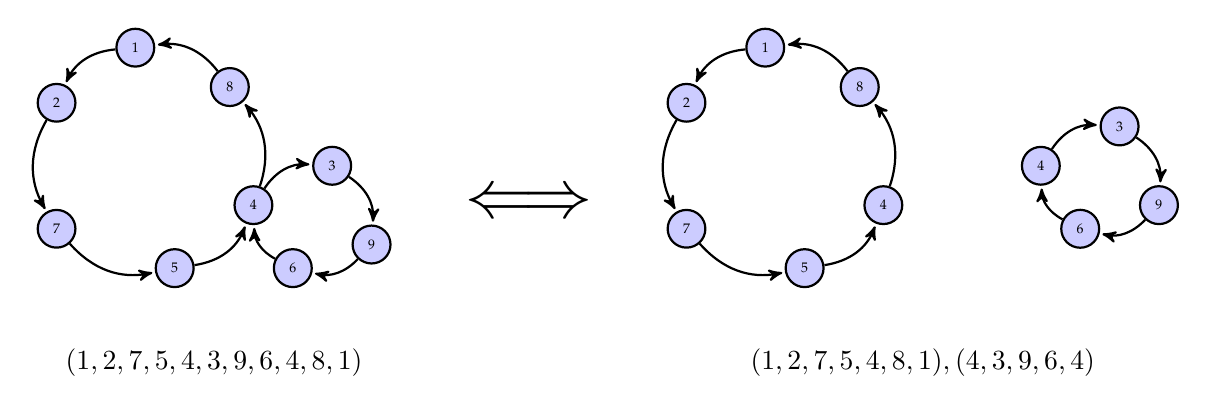
\begin{tikzpicture}[->,>=stealth',shorten >=1pt,auto,thick,main node/.style={circle,fill=blue!20,draw,font=\tiny}]
\node[main node] (v1) at (0,0) {1};
\node[main node] (v2) at (-1,-0.7) {2};
\node[main node] (v3) at (-1,-2.3) {7};
\node[main node] (v4) at (0.5,-2.8) {5};
\node[main node] (v5) at (1.5,-2) {4};
\node[main node] (v6) at (1.2,-0.5) {8};


\path[bend right] (v1) edge (v2)
(v2) edge (v3)
(v3) edge (v4)
(v4) edge (v5)
(v5) edge (v6)
(v6) edge (v1);


\node[main node] (v61) at (2.5,-1.5) {3};
\node[main node] (v62) at (3,-2.5) {9};
\node[main node] (v63) at (2,-2.8) {6};

\path[bend left] (v5) edge (v61)
(v61) edge (v62)
(v62) edge (v63)
(v63) edge (v5);
\node at (1,-4) {$(1,2,7,5,4,3,9,6,4,8,1)$};


\node[main node] (u1) at (8,0) {1};
\node[main node] (u2) at (7,-0.7) {2};
\node[main node] (u3) at (7,-2.3) {7};
\node[main node] (u4) at (8.5,-2.8) {5};
\node[main node] (u5) at (9.5,-2) {4};
\node[main node] (u6) at (9.2,-0.5) {8};
\path[bend right] (u1) edge (u2)
(u2) edge (u3)
(u3) edge (u4)
(u4) edge (u5)
(u5) edge (u6)
(u6) edge (u1);

\node[main node] (u60) at (11.5,-1.5) {4};
\node[main node] (u61) at (12.5,-1) {3};
\node[main node] (u62) at (13,-2) {9};
\node[main node] (u63) at (12,-2.3) {6};
\path[bend left] (u60) edge (u61)
(u61) edge (u62)
(u62) edge (u63)
(u63) edge (u60);
\node at (10,-4) {$(1,2,7,5,4,8,1),(4,3,9,6,4)$};

\node at (5,-2) {\Huge $\Longleftrightarrow$};
\end{tikzpicture}

It is not hard to see that the two operations in the two different cases are exact inverses of each other. Thus, this establishes a matching among all clow sequences that are not cycle covers, with every matched pair having opposing signs. Thus, the overall contribution of clow sequences that are not cycle covers is zero. 
\end{proofof}


\subsection{Completeness of the permanent}

The $\VNP$ completeness for the permanent is trickier, and uses a very clever gadget. The proof described here is a modification of the proof in B\"urgisser's book \cite{bur00}. This is the simplest proof that I am aware of currently. \\

Let $f(x_1,\dots, x_n) = \sum_\veca g(x_1,\dots, x_n, a_1,\dots, a_m)$ be in $\VNP$ with $g(\vecx, \vecy)$ computable by a formula of size $s$ (Theorem~\ref{thm:vnp-formula}). Like in the previous section, we can construct a graph $G$ (with weights being either scalars or variables in $\vecx$ or $\vecy$) such that the sum of weighted cycle covers is equal to $g(\vecx, \vecy)$. The goal is to now compute $\sum_\veca g(\vecx, \veca)$. \\

Let us consider a simpler case, where there is a variable $y \in \vecy$ such that there is just one edge in $e_y \in G$ with weight $y$. Can we transform the graph $G$ locally to compute $g' = g_{(y=0)} + g_{(y=1)}$? Note that since $y$ occurs only once in $G$, we have that $g = y \cdot g_1 + g_0$ where $g_1$ and $g_0$ are independent of $y$. Thus, the polynomial $g'$ can be written as $g_1 + 2 g_0$. One way to compute this is to transform the graph $G$ so that any cycle-cover of $G$ that includes the edge $e_y$ has the same weight as before, but every cycle-cover that does not include the edge $e_y$ has its weight multiplied by $2$. This can be achieved by splitting the edge $e_y$ in the middle with a new vertex $v$ with a self-loop of weight $2$:

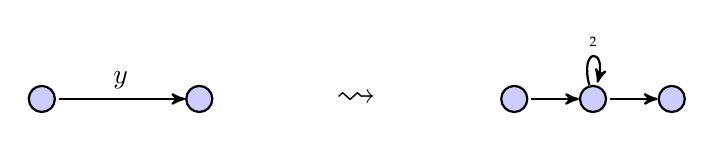
\begin{tikzpicture}[->,>=stealth',shorten >=1pt,auto,thick,main node/.style={circle,fill=blue!20,draw}]
\node[main node] (u) at (0,0) {};
\node[main node] (v) at (2,0) {}
edge[<-] node[above] {$y$} (u);
\node (arrow) at (4,0) {\Large $\leadsto$};
\node[main node] (u1) at (6,0) {};
\node[main node] (u2) at (7,0) {}
edge[<-] (u1);
\node[main node] (v1) at (8,0) {}
edge[<-] (u2);
\path[every node/.style={font=\tiny}] (u2) edge [loop above] node {2} (u2);
\end{tikzpicture}

Clearly, any cycle-cover that uses the edge $e_y$ has the same weight, and all other cycle-covers are forced to take the self-loop around the added vertex of weight $2$. This allows us to handle graphs $G$ where every variable $y \in \vecy$ occurs only once in $G$. The complication arises because there could be multiple edges that has the label $y$. We want a way by which we can say that all cycle covers that choose \emph{any} of the $y$-edges have the same weight, but cycle-covers that do not pick any $y$-edge have weight multiplied by $2$. The following is a gadget that has similar properties, called \emph{rosette}. The diagram below represents the $4$-rosette. 
\begin{center}
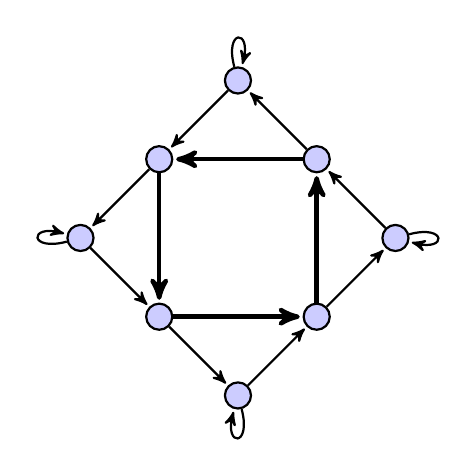
\begin{tikzpicture}[->,>=stealth',shorten >=1pt,auto,thick,main node/.style={circle,fill=blue!20,draw}]
\node[main node] (v1) at (0,0) {};
\node[main node] (v2) at (2,0) {};
\node[main node] (v3) at (2,2) {};
\node[main node] (v4) at (0,2) {};

\path[every node/.style={font=\tiny},ultra thick] (v1) edge (v2)
(v2) edge (v3)
(v3) edge (v4)
(v4) edge (v1);

\node[main node] (l1) at (1,-1) {};
\node[main node] (l2) at (3,1) {};
\node[main node] (l3) at (1,3) {};
\node[main node] (l4) at (-1,1) {};

\path[every node/.style={font=\tiny},thick] (l1) edge (v2)
edge [loop below] (l1)
(v2) edge (l2)
(l2) edge[loop right] (l2)
(l2) edge (v3)
(v3) edge (l3)
(l3) edge [loop above] (l3)
(l3) edge (v4)
(v4) edge (l4)
(l4) edge [loop left] (l4)
(l4) edge (v1) 
(v1) edge (l1);
\end{tikzpicture}
\end{center}
The thick edges in the above picture shall be called \emph{connector edges} (these shall play the role of the $y$-edges). Note that the rosette has the following two properties:
\begin{enumerate}
\item For any non-empty subset $S$ of the connector edges, there is exactly one cycle-cover of the rosette that includes exactly the set $S$ fo the connector-edges. 
\item There are exactly two cycle-covers of the rosette that do not include any connector edge. 
\end{enumerate}
Thus, if we could somehow ``glue'' the connector edges with our $y$-edges, we would be done. This is achieved by yet another gadget that we shall call the \emph{glue gadget}. The following is the description of the glue gadget that glues edges $(u,v)$ and $(u',v')$ by adding three additional vertices. 

\begin{center}
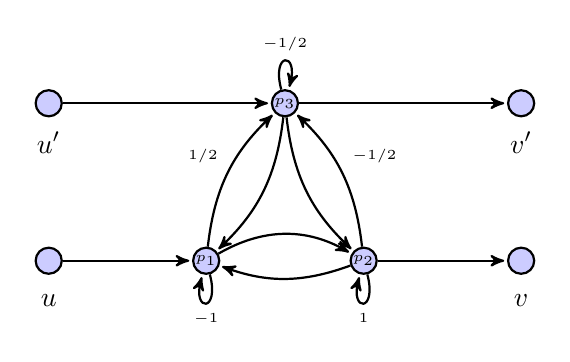
\begin{tikzpicture}[->,>=stealth',shorten >=1pt,auto,thick,main node/.style={circle,fill=blue!20,draw}]
\node[main node] (u) at (0,0) {};
\node (lu) at (0,-0.5) {$u$};
\node[main node] (v) at (6,0) {};
\node (lu) at (6,-0.5) {$v$};

\node[main node] (u1) at (0,2) {};
\node (lu1) at (0,1.5) {$u'$};

\node[main node] (v1) at (6,2) {};
\node (lv1) at (6,1.5) {$v'$};

\node[main node] (p1) at (2,0) {};
\node at (2,0) {\tiny $p_1$};

\node[main node] (p2) at (4,0) {};
\node at (4,0) {\tiny $p_2$};

\node[main node] (p3) at (3,2) {};
\node at (3,2) {\tiny $p_3$};

\path[every node/.style={font=\tiny},thick] (u) edge (p1)
(p1) edge [bend left] (p2)
(p2) edge (v)
(u1) edge (p3)
(p3) edge (v1)
(p3) edge [loop above] node {$-1/2$} (p3)
(p1) edge [bend left=20] node {$1/2$} (p3)
(p2) edge [bend right=20] node [above right] {$-1/2$} (p3)
(p3) edge [bend left=20] (p1)
(p3) edge [bend right=20] (p2)
(p1) edge [loop below] node {$-1$} (p1)
(p2) edge [loop below] node {$1$} (p2)
edge [bend left=20] (p1);
\end{tikzpicture}
\end{center}
The adjacency matrix between the nodes $p_1$, $p_2$ and $p_3$ is 
\[
A = \insquare{\begin{array}{rrr}
-1 & 1 & 1/2\\
1 & 1 & -1/2\\
1 & 1 & -1/2
\end{array}}
\]

\noindent
\begin{claim}
Let $(u,v)$ and $(u',v')$ be two edges of a graph $G$, and let $G'$ be the graph with the glue gadget between them as described above. Then $\mathrm{perm}(G')$ equals the sum of all weighted cycle covers of $G$ that either include both $(u,v)$ and $(u',v')$ in it or neither. 
\end{claim}
\begin{proof}
If both edges $(u,v)$ and $(u',v')$ are taken in the cycle cover, this is realised in $G'$ as ${(\cdots u,p_1, p_2, v \cdots) (\cdots u', p_3, v' \cdots)}$, which has the same weight.  

If neither of the edges $(u,v)$ and $(u',v')$ are taken in the cycle cover, then the total contribution of all cycle covers of $p_1$, $p_2$ and $p_3$ is $\mathrm{perm}(A) = 1$. 

If the edge $(u,v)$ is taken but $(u',v')$ is not, then the edge $(u,v)$ can be realised in $G'$ as either $\inbrace{(\cdots u,p_1,p_2,v \cdots) (p_3)}$ or $\inbrace{(\cdots u,p_1,p_3,p_2,v \cdots )}$. The total contribution is therefore zero. 

Similarly, if the edge $(u',v')$ is taken but not $(u,v)$, then this can be realised in $G'$ as $\inbrace{(\cdots u',p_3,v' \cdots),(p_1,p_2)}$ and $\inbrace{(\cdots u',p_3, v' \cdots) (p_1) (p_2)}$. Again, the net contribution is zero.  
\end{proof}

Now with these two gadgets, we are done. For every variable $y_i \in \vecy$, let $e_{i,1}, \dots, e_{i,r_i}$ be the edges labelled with $y$. Let $R_i$ be a $r_i$-rosette disjoint from the graph $G$ The graph $G'$ is built as follows:
\begin{quote}
  Take a disjoint union of $G$ with one $r_i$-rosette for each $i = 1,\dots, m$. 

  Glue each edge labelled with $y_i$ with the $r_i$ connector edges in the $r_i$-rosette. 
\end{quote}

It should be easy to see that $\mathrm{perm}(G) = \sum_{\veca} g(\vecx, \veca)$. This completes the proof of the $\VNP$-completeness of $\Perm_n$. \qed {\footnotesize (Theorem~\ref{thm:vnp})} \\

Note that we needed to divide by $2$ in the glue gadget. This is why we require the characteristic of the field to be different from two for the above proof to work. 

\begin{exercise}
  For any matrix $A$, we shall use the notation that $A[1|2]$ refers to the submatrix obtained by removing row $1$ and column $2$.

  Show that, for a three-vertex \emph{glue gadget}, you need a $3\times 3$ matrix $A$ that satisfies the following three properties:
  \begin{itemize}
    \item $\mathrm{perm}(A) = \mathrm{perm}(A[2,3|1,3]) = 1$. 
    \item $\mathrm{perm}(A[3|3]) = \mathrm{perm}(A[2|1]) = \mathrm{perm}(A[1|3]) = \mathrm{perm}(A[2|3]) = 0$.
  \end{itemize}
  
  Come up with an alternate construction of a matrix $A$ as a \emph{glue gadget}. Also prove that any such construction must involve entries of $A$ with its denominator divisible by $2$, and show that replacing $\mathrm{perm}$ by $\det$ above would yield no solution. 
\end{exercise}


%%% Local Variables: 
%%% mode: latex
%%% TeX-master: "main"
%%% End: 


\chapter{Some estimates for binomial coefficients}

Throughout this article, we would be seeing several binomial coefficients. The following estimates would allow us to get a better handle on the growth of such terms. 

We shall use $\log$ to refer to $\log_2$ and $\ln$ to refer to the natural logarithm. 


\begin{definition}[Entropy function]\label{def:entropy}
The binary entropy function $H_2:[0,1]\rightarrow [0,1]$ is defined as
\[
H_2(p) \quad = \quad - p \log_2(p) \spaced{-} (1-p) \log_2(1-p)
\]
The entropy function with respect to the natural logarithm is refer to as $H$ and
\[
H(p) \quad = \quad - p \ln(p) \spaced{-} (1-p) \ln(1-p)
\]
\end{definition}

\begin{proposition}\label{prop:entropy-estimate}
For any $0< p  < 1$, we have $p\ln\frac{1}{p} \leq H(p) \leq p\ln\frac{1}{p} + p$. 
\end{proposition}

\begin{proposition}[Sterling's Approximation]\label{prop:sterling}
\[
\log n! \quad=\quad n\log n - n + O(\log n)
\]
\end{proposition}

\begin{proposition}
For any constants $\alpha, \beta$, 
\[
\log\binom{\alpha n}{\beta n} \quad = \quad H_2\inparen{\frac{\beta}{\alpha}} \cdot \alpha n - O(\log n)
\]
In particular, if $\beta = \alpha/2$, then $\binom{\alpha n}{\beta{n}} = 2^{\alpha n} / \poly(n)$. 
\end{proposition}

For the more recent lower bounds, we would encounter several delicate ratios of binomial coefficients. The following lemma would help us simplify several such expressions and get a better handle on the growth. 

\begin{lemma}{\cite[Lemma 6]{gkks13}}\label{lem:factorial-ratio} For any $a,b = O(\sqrt{n})$, then
\[
\frac{(n+a)!}{(n-b)!}\quad=\quad n^{a + b} \cdot \poly(n)
\]
\end{lemma}

We shall be using the above lemma very often in the lower bounds. One particular instantiation that shall also appear frequently shall be the following lemma.  

\begin{lemma}\label{lem:binom-approx}
Let $n$ and $\ell$ be parameters such that $\ell = \frac{n}{2}(1 - \epsilon)$ for some $\epsilon = o(1)$. For any $a, b$ such that $a,b = O(\sqrt{n})$, 
\[
\binom{n - a}{\ell - b} \quad = \quad \binom{n}{\ell} \cdot 2^{-a} \cdot (1+\epsilon)^{a-2b} \cdot \poly(n)
\]
\end{lemma}
\begin{proof}
The proof of the above lemma would repeated use Lemma~\ref{lem:factorial-ratio}. 
\begin{eqnarray*}
\frac{\binom{n-a}{\ell -b}}{\binom{n}{\ell}} & = & \frac{(n-a)!}{n!} \cdot \frac{\ell!}{(\ell -b)!}\cdot \frac{(n-\ell)!}{(n-\ell-a+b)!}\\
& \stackrel{\poly}{\approx}& \frac{1}{n^a} \cdot \ell^b \cdot \frac{(n-\ell)^a}{(n-\ell)^b}\\
& = & \frac{\inparen{\frac{n}{2}}^a(1 +\epsilon)^a}{n^a} \cdot \frac{(1-\epsilon)^{b}}{(1+\epsilon)^b}\\
& \stackrel{\poly}{\approx} & 2^{-a} \cdot (1+\epsilon)^{a - 2b}
\end{eqnarray*}
\end{proof}


%%% Local Variables: 
%%% mode: latex
%%% TeX-master: "main"
%%% End: 


\chapter{Structural Results}\label{chap:structural-results}


This chapter shall be devoted to looking at some structural results on arithmetic circuits. This would help us understand the relevance of shallow circuits in the context of proving lower bounds for arithmetic circuits of arbitrary depth. 

\section{Homogenization}\label{sec:homogenization}

Suppose we have an $n$-variate degree $d$ polynomial computed by an arithmetic circuit $C$. How large can the degree of intermediate computations be? Potentially, intermediate computations can involve very high degree terms which somehow cancel each other at the root. However, the following lemma of Strassen shows that we may assume without much loss of generality that arithmetic circuits never compute polynomials of degree more than the output. 

\begin{definition}[Homogeneous circuits]
A circuit $C$ is said to be \emph{homogeneous} if every gate in the circuit computes a homogeneous polynomial. 
\end{definition}

\begin{lemma}[Homogenization]\label{lem:homogenization}
Let $f$ be an $n$-variate degree $d$ polynomial computed by a circuit $C$ of size $s$. Then, for every $0\leq i \leq d$, there is a \emph{homogeneous arithmetic circuit} $C_i'$, of size at most $O(sd^2)$, that computes the degree $i$ homogeneous polynomial in $i$. 
\end{lemma}
\begin{proof}
Assume without loss of generality that the circuit $C$ has all gates with fan-in at most $2$. 
For every gate $g\in C$, define $(d+1)$ gates $g^{(0)},\dots, g^{(d)}$; we shall construct a new circuit $C'$ such that $g^{(i)}$ computes the degree $i$ homogeneous component of the polynomial computed at $g$. If $g$ has children $h_1$ and $h_2$, then $C'$ would have the following connections depending on the type of the gate $g$:
\begin{eqnarray*}
\text{$g = h_1 + h_2$}\quad\implies\quad g^{(i)} &=& h_1^{(i)} \spaced{+} h_2^{(i)}\quad\text{for all $i$}\\
\text{$g = h_1 \times h_2$}\quad\implies\quad g^{(i)} &=& \sum_{j=0}^i h_1^{(j)} h_2^{(i-j)}\quad\text{for all $i$}
\end{eqnarray*}
It is easy to check that the size of the circuit $C'$ is at most $O(sd^2)$, and computes all the homogeneous components of $f$. 
\end{proof}

Thus, for arithmetic circuits, we can assume without much loss of generality that we are working with a homogeneous circuit. 

\begin{remark*}
For the class of arithmetic formulas, it is not clear if we can homogeneous without loss of generality. If we were to apply the above lemma to an arbitrary arithmetic formula, the resulting object is a homogeneous circuit and not a formula. It is unclear if any formula can be homogenized without loss of generality. The same is the case even for circuits of a fixed depth, as the above construction doubles the depth of the circuit. 

However, the class of ABPs can also be assumed to be homogeneous without loss of generality. We leave this as an exercise. 
\end{remark*}

\begin{exercise}
Prove a similar homogenization lemma for algebraic branching programs. 
\end{exercise}

\section{Depth reduction}

The phenomenon of simulating an arbitrary arithmetic circuit by a \emph{shallow} arithmetic circuit is called \emph{depth reduction}. Arithmetic circuits exhibit some remarkable depth reduction results, and we shall go over these in this section. 

\subsection{Depth reduction for arithmetic formulas}

The depth reduction for formulas is quite easy to describe. This would also serve as step towards understanding the depth reduction for arithmetic circuits. The following depth reduction is due to Brent~\cite{brent74}. 

\begin{lemma}[\cite{brent74}]\label{lem:formula-depth-reduction}
Let $f$ be an $n$-variate degree $d$ polynomial computed by an arithmetic formula $\Phi$ of size $s$. Then, $f$ can also be computed by a formula $\Phi'$ of size $s' = \poly(s,n,d)$ and depth $O(\log s)$. 
\end{lemma}
\begin{proof}
Assume without loss of generality that $\Phi$ is a formula of fan-in $2$. Starting from the root, walk down to the leaves by always taking the child with a larger sub-tree under it. Consider the first node in this path $v$ such that the size of the formula rooted at $v$ is smaller than $\frac{2s}{3}$. Let $\Phi_v$ refer to the sub-formula rooted at $v$. By the choice of the path from the root, we have
\[
\frac{s}{3} \spaced{\leq} \abs{\Phi_v} \spaced{<} \frac{2s}{3}.
\]
Let $\hat{\Phi}_v$ denote the formula where the sub-formula at $v$ is replaced by a fresh variable $y$. Since we are dealing with formulas, $\hat{\Phi}_v$ is a linear polynomial in the variable $y$. Hence,
\begin{eqnarray*}
\hat{\Phi}_v(y) & = & A \cdot y \spaced{+} B\\
\text{and,}\quad \Phi & = & A \cdot \Phi_v \spaced{+} B
\end{eqnarray*}
for some polynomials $A$ and $B$. But we can compute both $A$ and $B$ from $\hat{\Phi}_v(y)$ as
\begin{eqnarray*}
A & = & \hat{\Phi}_v(1) - \hat{\Phi}_v(0)\\
B & = & \hat{\Phi}_v(0)
\end{eqnarray*}
Thus, 
\[
f \quad = \quad (\hat{\Phi}_v(1) - \hat{\Phi}_v(0))\cdot \Phi_v \spaced{+} \hat{\Phi}_v(0)
\]
All the formulas in the above equation have size at most $\frac{2s}{3}$. Thus, by recursively applying this process on each of these sub-formulas, we obtain
\begin{eqnarray*}
\mathrm{Depth}(s) & = & \mathrm{Depth}(2s/3) \spaced{+} 3\\
\implies \mathrm{Depth}(s) &=& O(\log s)\\
\mathrm{Size}(s) & \leq & 3\cdot \mathrm{Size}(2s/3) \spaced{+} 3\\
\implies \mathrm{Size}(s) &=& \poly(s).
\end{eqnarray*}
\end{proof}

\begin{figure}
\begin{center}
\tikzstyle{gate}=[circle,draw=black!50,thick]
\tikzstyle{leaf}=[circle,draw=black!50,fill=black!10,thick]
\tikzstyle{phi}=[rectangle,draw=black!50,fill=black!10,thick]
\begin{tikzpicture}[transform shape, scale=0.7]
  \draw[fill=gray] (-10,-2) -- ++(-2,-2) -- ++(2,-2) -- ++(1,1) -- cycle;
  \draw[fill=gray!50] (-9,-5) -- ++(1,-3) -- ++(-2,2) -- cycle;

    \node at (-10,-1.3) {$f$}
    edge[<-,thick] (-10,-2) ;

  
  \node at (-7,-4) {\Huge $\longrightarrow$};
  
  \node (ph) at (-1,0) {$f$};
  \node[gate] (root) at (-1,-1) {$+$}
  edge[thick,->] (ph)
  edge[->] (4,-4.5);
  \node[gate] (m1) at (-2,-2) {$\times$}
  edge[->] (root)
  edge[->] (1,-4.5);
  
  \draw[fill=gray] (4,-4.5) -- ++(-2,-2) -- ++(2,-2) -- ++(1,1) -- cycle;
  \node at  (5.4,-7.8) { $0$}
  edge[<-] (5,-7.5);
  
  \node[gate] (s1) at (-3,-3) {$+$}
  edge[->] (m1)
  edge[->] (-4,-4.5)
  edge[->] node[above] {\tiny $-1$} (-1,-4.5);
  
  \draw[fill=gray!50] (1,-4.5) -- ++(1,-3) -- ++(-2,2) -- cycle;
  
  
  \draw[fill=gray] (-4,-4.5) -- ++(-2,-2) -- ++(2,-2) -- ++(1,1) -- cycle;
  \node at  (-2.6,-7.8) { $1$}
  edge[<-] (-3,-7.5);
  
  \draw[fill=gray] (-1,-4.5) -- ++(-2,-2) -- ++(2,-2) -- ++(1,1) -- cycle;
  \node at  (0.4,-7.8) { $0$}
  edge[<-] (0,-7.5);
\end{tikzpicture}
\end{center}
\caption{Depth reduction for formulas}
\label{fig:formula-depth-red}
\end{figure}

\subsection{Depth reduction for arithmetic circuits}

The key point in the above depth reduction was that for any node $v$, the formulas $\Phi_v$ and $\hat{\Phi}_v(y)$ were disjoint. This however is not the case for general arithmetic circuits. Thus, it is not clear if we can find a node in the circuit such that the subcircuit under it has size between $s/3$ and $2s/3$. However, we do not really need to make the subcircuits have size drop by a constant factor, but any parameter dropping by a constant factor would be fine. One parameter that we could work with instead is the \emph{degree}. 


\subsubsection{Applying Brent's reduction with degree}

By Lemma~\ref{lem:homogenization}, we may assume that we have a homogeneous circuit $\Phi$ if size $s$ computing a homogeneous $n$-variate polynomial $f$ of degree $d$. Using a similar argument as in the proof of Lemma~\ref{lem:formula-depth-reduction}, we can find a node $v \in \Phi$ such that $\frac{d}{3} < \deg(v) \leq \frac{2d}{3}$. However, we cannot quite write $f$ as $A \cdot \Phi_v + B$ as we are now dealing with a circuit and there could be multiple paths from the root leading to $v$.

Consider the set of all nodes of such intermediate degree as $\mathcal{F}$:
\[
\mathcal{F} = \setdef{v\in \Phi}{\frac{d}{3} < \deg(v)\leq \frac{2d}{3}}
\]
Instead of expressing $f$ using a single $v\in \mathcal{F}$ as in Lemma~\ref{lem:formula-depth-reduction}, we shall express $f$ as a function of \emph{all} nodes in $\mathcal{F}$. 

\begin{claim}
If $\mathcal{F} = \inbrace{v_1,\dots, v_s}$, then $f$ may be written as
\begin{equation}\label{eqn:hyafil}
f \spaced{=} \sum_{i,j} A_{ij} \cdot \Phi_{v_i} \Phi_{v_j} \spaced{+} \sum_i B_i \cdot \Phi_{v_i}
\end{equation}
where $\deg(A_{ij}), \deg(B_i) \leq \frac{2d}{3}$ for all $i,j$. Moreover, each $A_{ij}$ and $B_i$'s may be computed by an arithmetic circuit of size at most $O(s)$. 
\end{claim}
\begin{proof}
From the circuit $\Phi$, construct the circuit $\Phi'$ that is obtained by removing the incoming edges of every $v_i \in \mathcal{F}$ thereby making these nodes as leaves as well. Then, $\Phi'$ computes a polynomial $f'(x_1,\dots x_n, v_1,\dots, v_s)$ satisfying 
\[
f \spaced{=} f'(x_1,\dots, x_n, \Phi_{v_1},\dots, \Phi_{v_s}).
\]
Because of the degree of each $v_i$, we easily obtain that the degree of $f'$ in the $v_i$ variables must be at most $2$, and each coefficient $A_{ij}$ or $B_i$ cannot have degree more than $2d/3$. Further, obtaining the $A_{ij}$'s and $B_i$'s from $\Phi'$ is a simple exercise. 
\end{proof}

Since every polynomial appearing in \eqref{eqn:hyafil} is computable by size at most $\poly(s)$ and has degree at most $2d/3$, we may apply induction as earlier. Thus,
\begin{eqnarray*}
\mathrm{Depth}(d) & = & \mathrm{Depth}(2d/3) \quad + 2\\
\implies \mathrm{Depth}(d) & = & O(\log d)
\end{eqnarray*}
Unfortunately, the size of the resulting circuit could be as large as $s^{O(\log d)}$.  This reduction is along the lines of Hyafil~\cite{Hyafil1978}. 

Notice that in this reduction, the final circuit we obtain is in fact an arithmetic formula of size $s^{O(\log d)}$ and depth $O(\log d)$ (assuming that addition gates can have unbounded fan-in; with bounded fan-in addition gates, the depth would be $O(\log d \cdot \log s)$). Valiant, Skyum Berkowitz and Rackoff \cite{vsbr83} showed that we can attain a similar depth reduction to $O(\log d)$ depth while keeping the size polynomial. 


\subsubsection{Depth reduction of \cite{vsbr83}}


This section shall be devoted to the proof of the remarkable theorem of Valiant, Skyum, Berkowitz and Rackoff.\footnote{The proof described here follows the structure of a subsequent result \cite{ajmv98}, and not the original proof, although both proofs are quite similar.}


\begin{theorem}[\cite{vsbr83,ajmv98}]\label{thm:vsbr}
  Let $f$ be an $n$-variate degree $d$ polynomial computed by an
  arithmetic circuit $\Phi$ of size $s$. Then there is an arithmetic
  circuit $\Phi'$ computing $f$ and has size $s' = \poly(s,n,d)$ and
  depth $O(\log d)$.
\end{theorem}

We may assume without loss of generality that $\Phi$ is a homogeneous circuit. We will also assume that all multiplication gates in $\Phi$ have fan-in at most $2$, and also that the degree of the right child of any multiplication gate is at least as large as the degree of the left child. Such circuits are also referred to as \emph{right heavy} circuits. We shall need the following definition of gate quotients.

\begin{definition}\label{defn:gate-quotient}
For any pair of gates $u,v$, the polynomial $[u:v]$ is defined as follows:
\begin{enumerate}
\item If $u$ and $v$ are the same nodes, then $[u:v] = 1$. 
\item If $u$ is a leaf, and $u\neq v$, then $[u:v] = 0$. 
\item If $u = u_1 + u_2$, then $[u:v] = [u_1:v] + [u_2:v]$.
\item If $u = u_1 \times u_2$, then $[u:v] = [u_1] \cdot [u_2 : v]$. 
\end{enumerate}
\end{definition}

It is easy to see that $[u:v]$ is a homogeneous polynomial of degree $\deg(u) - \deg(v)$. 
To understand this definition better, consider the case of a formula instead of a circuit. Then for any node $u$, and another node $v$ in the sub-formula rooted at $u$, the polynomial $[u]$ can depends on $[v]$ linearly as $[u] = A [v] + B$ for some $A,B$. In this setting, $[u:v] = A$. For circuits however, there could be multiple paths from $u$ leading to $v$. One possible alternate definition could have been to \emph{differentiate} $[u]$ by $[v]$ but this would require some additional care. The above definition makes sure we are exploring only one of the children of any multiplication gate, and yields a much simpler proof. 

\begin{definition}[Frontier]\label{defn:frontier}
For any parameter $a$, define the \emph{frontier at degree $a$} as
\[
\mathcal{F}_a \quad=\quad \setdef{v}{\deg(v) \geq a\;,\; \deg(v_L), \deg(v_R) < a}
\]
That is, $\mathcal{F}_a$ are the deepest nodes in the circuit that have degree at least $a$. 
\end{definition}

Note that from the above definition, all frontier nodes are multiplication gates (since we are working with a homogeneous circuit). Also, if $v_1,v_2$ are two distinct nodes in $\mathcal{F}_a$, then $v_1$ does not occur in the sub-circuit rooted at $v_2$ (and vice-versa). 

\begin{observation}\label{obs:vsbr-antichain}
If a node $v$ does not occur in the sub-formula rooted at $u$, then $[u:v] = 0$. In particular, if $u\neq v\in \mathcal{F}_a$ for some $a$, then $[u:v]=0$.
\end{observation}

The following is the key lemma for the depth reduction. 

\begin{lemma}
Suppose $\Phi$ is a homogeneous, right-heavy circuit. Let $a$ be a parameter such that $\deg(u) \geq a$. Then,
\begin{equation}\label{eqn:vsbr-for-u}
[u]\spaced{=} \sum_{w\in \mathcal{F}_a} [u:w] \cdot [w]
\end{equation}
Also, if $u,v$ are nodes such that $\deg(u) \geq a > \deg(v)$, then
\begin{equation}\label{eqn:vsbr-for-uv}
[u:v] \spaced{=} \sum_{w\in \mathcal{F}_a} [u:w] [w:v]
\end{equation}
\end{lemma}
\begin{proof}
The proof would be by induction on the depth of $u$. Note that if $u = u_1 + u_2$, then it follows immediately that 
\begin{eqnarray*}
  [u] &=& [u_1] + [u_2] \\
  &=& \sum_{w\in \mathcal{F}_a} \inparen{[u_1: w]\cdot [w]  + [u_2:w]\cdot [w]}\quad\text{(inductive hypothesis)}\\
  &=& \sum_{w\in \mathcal{F}_a} [u:w] \cdot [w] \quad\text{(Definition~\ref{defn:gate-quotient})}
\end{eqnarray*}
\begin{eqnarray*}
  [u:v] &=& [u_1:v] + [u_2:v] \\
  &=& \sum_{w\in \mathcal{F}_a} \inparen{[u_1: w]\cdot [w:v]  + [u_2:w]\cdot [w:v]}\quad\text{(inductive hypothesis)}\\
  &=& \sum_{w\in \mathcal{F}_a} [u:w] \cdot [w:v] \quad\text{(Definition~\ref{defn:gate-quotient})}
\end{eqnarray*}
Suppose $u = u_1 \times u_2$. If $\deg(u_2) \geq a$ as well, then by induction we have
\begin{eqnarray*}
[u] &=& [u_1] \cdot [u_2]\\
    &=& [u_1] \cdot \inparen{\sum_{w\in \mathcal{F}_a} [u_2:w]\cdot [w]} \quad\text{(inductive hypothesis)}\\
    &=& \sum_{w\in \mathcal{F}_a}([u_1]\cdot [u_2:w]) \cdot [w] = \sum_{w\in \mathcal{F}_a}[u:w] \cdot [w]\quad\text{(Definition~\ref{defn:gate-quotient})}
\end{eqnarray*}
\begin{eqnarray*}
[u:v] &=& [u_1] \cdot [u_2:v]\\
    &=& [u_1] \cdot \inparen{\sum_{w\in \mathcal{F}_a} [u_2:w]\cdot [w:v]} \quad\text{(inductive hypothesis)}\\
    &=& \sum_{w\in \mathcal{F}_a}([u_1]\cdot [u_2:w]) \cdot [w:v] = \sum_{w\in \mathcal{F}_a}[u:w] \cdot [w:v]\quad\text{(Definition~\ref{defn:gate-quotient})}
\end{eqnarray*}

If $\deg(u_2) < a$, then note that $u \in \mathcal{F}_a$. Hence,
\begin{eqnarray*}
\sum_{w\in \mathcal{F}_a} [u:w] \cdot [w] &=& [u:u] \cdot [u] \spaced{+}\sum_{\substack{w\in \mathcal{F}_a\\w\neq u}} [u:w] \cdot [w] \spaced{=} [u] \spaced{+} 0\\
\sum_{w\in \mathcal{F}_a} [u:w] \cdot [w:v] &=& [u:u] \cdot [u:v] \spaced{+}\sum_{\substack{w\in \mathcal{F}_a\\w\neq u}} [u:w] \cdot [w:v] \spaced{=} [u:v] \spaced{+} 0
\end{eqnarray*}
as $[u:w] = 0$ for all $u\neq w \in \mathcal{F}_a$ (Observation~\ref{obs:vsbr-antichain}).
\end{proof}

Now we are ready to write down the depth reduced circuit. The original proof of \cite{vsbr83} follows a bottom-up approach, but it would be more useful to us to take a top-down approach (as in \cite{ajmv98}) to obtain some additional structural properties that we would require. \\

\begin{theorem}
Let $\Phi$ be a homogeneous, left-heavy circuit of size $s$ computing an $n$-variate degree $d$ polynomial. Then, there is a circuit $\Phi'$ of size $\poly(s)$ with the following properties:
\begin{enumerate}
\item For every $u\in \Phi$, there is a node in $\Phi'$ that computes $[u]$.
\item For every $u,v\in \Phi$, there is a node in $\Phi'$ that computes $[u:v]$. 
\item All addition gates in $\Phi'$ have fan-in at most $s^2$. 
\item All multiplication gates in $\Phi'$ have fan-in at most $5$. 
\item For every multiplication gate in $\Phi'$, all its children have at most half its degree. 
\end{enumerate}
\end{theorem}
\begin{proof}
All nodes $[u]$ and $[u:v]$ of degree at most $1$ are linear polynomials, and hence can are written down explicitly in $\Phi'$. 

For any node $u\in \Phi$, let $\mathcal{F}(u) = \mathcal{F}_a$ for $a = \deg(u)/2$. Thus by \eqref{eqn:vsbr-for-u},
\begin{eqnarray*}
[u] & = & \sum_{w\in \mathcal{F}(u)} [u:w] \cdot [w]\\ 
    & = & \sum_{w\in \mathcal{F}(u)} [u:w] \cdot [w_L] \cdot [w_R]
\end{eqnarray*}
Note that by the choice of $a$, all the terms on the RHS have degree at most $\deg(u)/2$. 

For any pair of nodes $u,v\in \Phi$, let $\mathcal{F}(u,v) = \mathcal{F}_a$ for $a = (\deg(u) + \deg(v))/2$. By \eqref{eqn:vsbr-for-uv},
\begin{eqnarray*}
[u:v] & = & \sum_{w\in \mathcal{F}(u,v)} [u:w] \cdot [w:v]\\ 
    & = & \sum_{w\in \mathcal{F}(u,v)} [u:w] \cdot [w_L] \cdot [w_R:v]
\end{eqnarray*}
Again by the choice of $a$, the degree of $[u:w]$ and the degree of $[w_R:v]$ is at most $(\deg(u) - \deg(v))/2$. The degree of $[w_L]$ however could be as large as $\deg(u) - \deg(v)$. Nevertheless, we can use the above expansion once more to write it as
\begin{eqnarray*}
  [u:v] & = & \sum_{w\in \mathcal{F}(u,v)} [u:w] \cdot [w_L] \cdot [w_R:v]\\
        & = & \sum_{w\in \mathcal{F}(u,v)} [u:w] \inparen{\sum_{p \in \mathcal{F}(w_L)} [w_L:p] \cdot [p_L] \cdot [p_R]}\cdot [w_R:v]\\
        & = & \sum_{w\in \mathcal{F}(u,v)}\sum_{p\in \mathcal{F}(w_L)} [u_w] \cdot  [w_L:p] \cdot [p_L] \cdot [p_R]\cdot [w_R:v]
\end{eqnarray*}
Now all the terms on the RHS have degree at most $(\deg(u) - \deg(v))/2$ as required. 
\end{proof}

% \newpage



% \begin{theorem}[\cite{vsbr83}]\label{thm:vsbr}
% Let $f$ be an $n$-variate degree $d$ polynomial computed by an arithmetic circuit $\Phi$ of size $s$. Then, there is an arithmetic circuit $\Phi'$ computing $f$ and has size $s' = \poly(s,n,d)$ and depth $O(\log d)$. 
% \end{theorem}

% By Lemma~\ref{lem:homogenization}, we may assume without loss of generality that $\Phi$ is a homogeneous circuit. We will also assume that in $\Phi$, all multiplication gates have fan-in at most $2$ (this might increase the depth of $\Phi$ by a factor of $\log s$, but this would not hurt us). Now, we can find a similar ``$\inparen{\frac{1}{3},\frac{2}{3}}$ separator'' as in the proof of Lemma~\ref{lem:formula-depth-reduction}, but based on degree instead of size. 

% \begin{claim}
% Let $\Phi$ be a homogeneous arithmetic circuit computing a homogeneous degree $d$ polynomial, where each multiplication gate has fan-in at most $2$. Then, there exists a node $v$ that computes a polynomial of degree $d'$ satisfying $d/3 \leq d' \leq 2d/3$. 
% \end{claim}

% The proof is exactly the same, except now you take a path from root to leaf by always going through the child of larger degree. What can we say about replacing the entire sub-circuit at $v$ by a new variable $y$? This runs in to some immediate problems. What if there was a node $w$ in the subcircuit at $v$, which is maybe connected to other nodes in $\Phi$? Also, the polynomial $\hat{\Phi}_v(y)$ could continue to have degree as large as $d$. Thus it is not clear if this approach would help us make progress. 

% The cause of all these problems stems because the node $v$ could reached from the root through multiple paths, and hence needs to be treated with care. However, with a little more care, we can still mimic the earlier depth reduction for formulas. \\

% Let us go over every gate in $\Phi$, and reorder the children so that the children are sorted in decreasing order of degrees (with the left child being the one with largest degree). We shall call such circuits as \emph{left-heavy} circuits. Note that the proof of the claim above yields such a node $v$ on the left-most path of $\Phi$. 

% Since any polynomial is a sum of monomials, it would be useful to break the computation by an arbitrary circuits by a sum of smaller computations each corresponding to a monomial. The following definition does just that. 

% \begin{definition}[Proof trees]\label{defn:proof-tree}
% A \emph{proof tree} of an arithmetic circuit $C$ is a sub-graph $T$ obtained as follows:
% \begin{itemize}
% \item The root of $C$ is in $T$.
% \item For every addition gate $g\in T$, the subgraph $T$ also contains \emph{exactly one} of its children.
% \item For every multiplication gate $g\in T$, the subgraph $T$ also contains \emph{both} its children. 
% \end{itemize}
% \end{definition}

% A proof tree naturally computes a single monomial, and is a minimal witness that a certain monomial is computed in by the circuit. (It is however possible that the same monomial can be computed by multiple proof trees and there could be several cancellations.)

% A very natural question at this point is why is a \emph{proof tree} a tree! It isn't clear from the above definition but note that all proof trees of a homogeneous circuit $C$ (computing a degree $d$ polynomial) computes a monomial of degree $d$. Thus, the number of multiplication gates in any proof tree is at most $d$. Thus, we may unravel any proof tree $T$ to an actual tree $T$ while not increasing the size by much. Thus, without loss of generality, we may assume that all proof trees of $C$ are unravelled to indeed be trees. 

% We shall denote the set of all proof trees of a circuit $C$ by $\mathrm{ProofTrees}(C)$. Also, for any node $u\in C$, we shall use $\mathrm{ProofTree}(u)$ to refer to the set of all proof trees rooted at $u$. Further, for any proof tree $T$, we shall use $\mathrm{eval}(T)$ to denote  the  \emph{monomial computed by $T$}. Thus, if $f$ is the polynomial computed by a circuit $C$, then
% \[
% f\spaced{=} \sum_{T\in \mathrm{ProofTrees}(C)} \mathrm{eval}(T)
% \]

% With this definition, we can now apply a Brent-like argument on \emph{proof trees} rather than the actual circuit itself. Recall that in the proof of Lemma~\ref{lem:formula-depth-reduction}, we expressed $\Phi$ as a linear function of $A \Phi_v + B$. The following notation captures the quotient $A$, but now in the case of general circuits via the notation of proof trees. 

% \begin{definition}[Proof tree quotients]
% For any proof tree $T$, and a node $v$, define the operation $\mathrm{snip}_v(T)$ as
% \begin{itemize}
%   \item If $v$ does not appear in the left-most path of $T$, then $\mathrm{snip}_v(T) = 0$
%   \item If $v$ does appear in the left-most path of $T$, then $\mathrm{snip}_v(T)$ refers to the tree obtained by replacing the node $v$ on the left-most path by a leaf labelled $1$. 
% \end{itemize}
% For any two nodes $u$ and $v$ in the circuit $C$, the polynomial $[u:v]$ is defined as
% \[
% [u:v] \spaced{=} \sum_{T \in \mathrm{ProofTrees}(u)} \mathrm{eval}(\mathrm{snip}_v(T))
% \]
% \end{definition}

% Intuitively, $[u:v]$ refers to the \emph{suffix} of $v$ in the computation at $u$. By only snipping off $v$ from the left-most path, this allows us to get a better control with the issue of $v$ occurring multiple times in the proof tree. For a formula $\Phi$, the polynomial $[\Phi:v]$ would refer to $\hat{\Phi}_v(1)$. Note that $[u:v]$ is a polynomial of degree $\deg(u) - \deg(v)$. \\

% The next thing we would like to do using the above notation is to rewrite the polynomial computed at $u$ by a sum involving several $[u:v_i]$s for suitable choice of $v_i$. To do this, we need to identify a set of nodes $\inbrace{v_i}$ such that the left-most path of every proof tree $T$ passes through exactly one $v_i$ from this set. One example of such a set is just the set of leaves. Thus, we can express the polynomial computed at any node $u$ as
% \[
% [u] \spaced{=} \sum_{i} [u:x_i] \cdot x_i
% \]
% In fact, a more general construction could be defined for any parameter $t$ as
% \[
% \mathcal{F}_t  \spaced{=} \setdef{w\in C}{\deg(w) \geq t \spaced{\&} \deg(w_L) < t}
% \]
% where $w_L$ refers to the left child of $w$. 

% \begin{observation}\label{obs:vsbr-split-threshold}
% For any node $u$, and a parameter $t$ such that $t \leq \deg(u)$, the left-most path of any proof tree $T$ of $u$ passes through exactly one node in $\mathcal{F}_t$. 
% \end{observation}

% Hence, $[u]$ can be expressed as follows:
% \begin{equation}\label{eqn:vsbr-split-threshold}
% [u] \spaced{=} \sum_{v\in \mathcal{F}_t} [u:v] \cdot [v]
% \end{equation}
% as long as $t \leq \deg(u)$. When we have nodes $u,v \in C$, we shall use $\mathrm{Frontier}(u)$ to refer to $\mathcal{F}_t$ where $t = \deg(u)/2$ and $\mathrm{Frontier}(u:v)$ to refer to $\mathcal{F}_t$ for $t = \deg(u:v)/2$. These are the frontiers that cut the appropriate tree into `half'. It is worth noting that all nodes in $\mathcal{F}_t$ must be multiplication gates (since the children have strictly smaller degree). 


% \begin{observation}
% The left-most path of any proof tree $T$ of $u$ passes through exactly one node in $\mathrm{Frontier}(u)$. The same applies to $\mathrm{Frontier}(u:v)$ as well. 
% \end{observation}

% With this observation, we have the sums we were looking for. 

% \begin{eqnarray}\label{eqn:VSBR-split-frontier}
% \text{For any $u\in C$,}\quad\quad [u] &=& \sum_{v\in \mathrm{Frontier}(u)} [u:v]\cdot [v] \label{eqn:VSBR-split-frontier-u}\\
% \text{For any $u,v\in C$,}\quad\quad [u:v] &=& \sum_{w\in \mathrm{Frontier}(u:v)} [u:w]\cdot [w:v] \label{eqn:VSBR-split-frontier-u:v}
% \end{eqnarray}

% With these in hand, we can now describe the depth-reduced circuit of \cite{vsbr83}. \\

% For each $u \in C$, the circuit $C'$ has a node computing $[u]$, and for every pair of nodes $u,v\in C$, there is a node in $C'$ computing $[u:v]$. To describe how $[u]$ is computed in $C'$, start with equation \eqref{eqn:VSBR-split-frontier-u}
% \begin{eqnarray*}
% [u] &=& \sum_{v\in \mathrm{Frontier}(u)} [u:v]\cdot [v]\\
%  & = & \sum_{v\in \mathrm{Frontier}(u)} [u:v] \cdot [v_L] \cdot [v_R]
% \end{eqnarray*}
% Note that since $v\in \mathrm{Frontier}(u)$, we have that $\deg(v) \geq \deg(u)/2$ and $\deg(v_R),\deg(v_L) < \deg(u)/2$. Thus each of the three terms in every summand of the above equation has degree at most half the degree $u$. The computation of $[u:v]$'s are a little more involved. By equation \eqref{eqn:VSBR-split-frontier-u:v}, we have
% \begin{eqnarray*}
% [u:v] &=& \sum_{w\in \mathrm{Frontier}(u:v)} [u:w]\cdot [w:v]\\
%       &=& \sum_{w\in \mathrm{Frontier}(u:v)} [u:w]\cdot [w_R]\cdot  [w_L:v]
% \end{eqnarray*}
% Since every $w \in \mathrm{Frontier}(u:v)$, we have that $\deg(u:w),\deg(w_L:v) \leq \deg(u:v)/2$. The issue is that $[w_R]$ could have pretty large degree. To see this, note that $w$ is a node of degree between $\deg(u)$ and $\deg(v)$. Thus, it is possible that $(u:w)$ and $(w_L:v)$ have very small degree and $\deg(w_R)$ could be as large as $\deg(u:v)$. However, we can expand $[w_R]$ using \eqref{eqn:VSBR-split-frontier-u} and we would then have what we want. 
% \begin{eqnarray*}
% [u:v] &=& \sum_{w\in \mathrm{Frontier}(u:v)} [u:w]\cdot [w_R]\cdot  [w_L:v]\\
%       &=& \sum_{w\in \mathrm{Frontier}(u:v)} [u:w]\cdot \inparen{\sum_{p \in \mathrm{Frontier}(w_L)} [w_R:p] \cdot [p_L] \cdot [p_R]} \cdot  [w_L:v]
% \end{eqnarray*}
% Observe that we have $\deg (u:w), \deg(w_L:v) \leq \deg(u:v)/2$ from earlier, and we also have
% \begin{eqnarray*}
% \deg(u:w),\deg(w_L:v) & \leq &\frac{\deg(u:v)}{2}\\
% \deg(w_R:p),\deg(p_L),\deg(p_R) & \leq & \frac{\deg(w_R)}{2}\\
%  & \leq & \frac{\deg(u:v)}{2}
% \end{eqnarray*}
% Thus, once again, we are in the situation where all the factors in the RHS have at most half the degree of the RHS. Thus, this shows that every $(u:v)$ can be computed by an arithmetic circuit $C'$ of size $\poly(s)$ and depth $O(\log d)$. In particular, $f = [\mathrm{root}]$ can be computed be computed by $C'$, as claimed. \qed {(\footnotesize Theorem~\ref{thm:vsbr})}\\

\begin{remark}\label{remark:vsbr}
From the proof above, we can see that the resulting circuit $\Phi'$ has useful structural properties. 
\begin{itemize}
  \item The circuit is homogeneous. 
  \item Addition gates have fan-in bounded by $\poly(s)$. 
  \item Multiplication gates have fan-in bounded by $5$. 
  \item If $u$ is any multiplication gate, then all its children $v$ satisfy $\deg(v)\leq \deg(u)/2$. 
\end{itemize}
\end{remark}

These additional properties would be useful in the next section, where we shall squash $\Phi'$ down to a depth four circuit!

\subsection{Reduction to depth four circuits}

One of the consequence of a depth reduction such as Theorem~\ref{thm:vsbr} is that proving lower bounds for general circuits is reduced to the task of proving lower bounds for $O(\log d)$ depth circuits. 

\begin{corollary}\label{cor:vsbr-contra}
If $f$ is an $n$-variate degree $d$ polynomial that requires super-polynomial (in $n$ and $d$) size circuits of $O(\log d)$ depth to compute it, then any general arithmetic circuit computing $f$ must also be of super-polynomial size. 
\end{corollary}

But, optimistically, we would expect that the \emph{right} lower bound must be truly exponential, and not merely super-polynomial. Keeping that in mind, a depth reduction even with a slightly super-polynomial blow-up might be useful in this regard. This line was first pursued by Agrawal and Vinay \cite{av08}, and the result was subsequently strengthened by Koiran \cite{koiran} and Tavenas~\cite{Tav13}. 

\begin{theorem}[\cite{av08,koiran,Tav13}] \label{thm:av}
Let $f$ be an $n$-variate degree $d$ polynomial computed by a size $s$ arithmetic circuit. Then for any $0< t \leq d$, $f$ can be equivalently computed by a homogeneous $\SPSP^{[t]}$ circuit of top fan-in $s^{O(d/t)}$ and size $s^{O(t + d/t)}$. 
\end{theorem}

If we were to optimize the size of the final depth four circuit, then we should choose $t = \sqrt{d}$ to get a $\SPSP^{[t]}$ circuit of size $s^{O(\sqrt{d})}$. Note that this implies that if we could prove a lower bound of $n^{\omega(\sqrt{d})}$ for such $\SPSP^{[\sqrt{d}]}$ circuits, then we would have proved a lower bound for general circuits! In fact, in the recent past, we have come pretty close to the required threshold and we shall see them in the later chapters. \\

In this section, we shall see a proof of Theorem~\ref{thm:av} but this is not the original proof of Tavenas~\cite{Tav13}. We shall see an alternate proof by \cite{saptharishivinay14}, which I find more insightful. 

\begin{proofof}{Theorem~\ref{thm:av}}
Let $C$ be the $O(\log d)$ depth  circuit computing $f$ obtained from Theorem~\ref{thm:vsbr} applied on the size $s$ circuit computing $f$. Let $s'$ be the size of $C$. If $g$ is a polynomial computed at any intermediate node of $C$, then from the structure of $C$ (Remark~\ref{remark:vsbr}) we have a homogeneous expression
\begin{equation}\label{eqn:vsbr-expansion}
g \spaced{=} \sum_{i=1}^{s'} g_{i1} \cdot g_{i2} \cdot g_{i3} \cdot g_{i4} \cdot g_{i5} 
\end{equation}
where each $g_{ij}$ is computed by a node in $C$ as well, and $\deg(g_{ij}) \leq \deg(g)/2$. If we look at \eqref{eqn:vsbr-expansion} for $f$, then the RHS is a $\SPSP^{[d/2]}$ circuit of top fan-in $s'$ computing $f$. To obtain a $\SPSP^{[t]}$ circuit eventually, we shall do the following natural process. 
\begin{quote}
  For each summand $g_{i1}\dots g_{ir}$ in the RHS, if the largest degree $g_{ij}$ has degree more than $t$, expand that $g_{ij}$ in-place using \eqref{eqn:vsbr-expansion}. 
  
  Repeat this process until all $g_{ij}$'s on the RHS have degree at most $t$. 
\end{quote}

Note that in each iteration of the above procedure, we increase the top fan-in by a multiplicative factor of $s'$, and what we gain is that some the terms in the RHS would now have smaller degrees. If we could show that the in $O(d/t)$  iterations  all terms on the RHS have degree at most $t$, then we would have obtained an $\SPSP^{[t]}$ circuit of top fanin $s'^{O(d/t)}$ computing $f$. \\

To bound the number of iterations, let us count the number of terms of degree more than $t/8$ in each term. Note that since we would always maintain homogeneity, the number of terms of degree  $t/8$ or more in any summand  is at most $8d/t$. Thus, it suffices to show that each iteration increases the number of terms of degree $t/8$ by at least one. 

Note that in \eqref{eqn:vsbr-expansion}, if $\deg(g) = d'$ then the largest degree term of any summand on the RHS is at least $d'/5$ (since the sum of the degrees of the five terms must add up to $d'$). Also, the largest degree term can have degree at most $d'/2$. Hence there must be at least $d'/2$ degree contributed by the other four factors in each term. This implies that the second largest factor in each summand has degree at least $d'/8$. Therefore, as long as we are expanding factors using \eqref{eqn:vsbr-expansion} of degree more than $t/8$, we are guaranteed that each new term has at least one more factor of degree more than $t/8$. As argued earlier, we can never have more than $8d/t$ such terms in any summand and this bounds the number of iterations by $8d/t$. 

Thus, when the above procedure stops, we have an $\SPSP^{[t]}$ circuit of top fan-in $s'^{O(8d/t)} = s^{O(d/t)}$. Observing that any polynomial of degree $t$ can have at most $n^t$ monomials, we get that the size of the circuit overall is at most $s^{O(t + d/t)}$. 
\end{proofof}

Thus, proving a ``good enough'' top fanin (or size) lower bound for the class of $\SPSP^{[t]}$ circuit would suffice for proving lower bounds for general circuits. We would be using this fact quite a lot so we state this explicitly as a corollary. 

\begin{corollary}\label{cor:av}
If $f$ is an $n$-variate degree $d$ polynomial that requires homogeneous $\SPSP^{[t]}$ circuits of top fan-in $n^{\omega(d/t)}$ to compute it, then $f$ requires general arithmetic circuits of size $n^{\omega(1)}$ to compute it. 
\end{corollary}

\begin{exercise}
Define the product-depth of any circuit to be the maximum number of multiplication gates encountered on any root-to-leaf path. 

Show that for any polynomial $n$-variate degree $d$ polynomial $f$ that can be computed by a size $s$ arithmetic circuit, there is a circuit $\Phi'$ of size $s^{O(d^{1/\Delta})}$ and product depth $\Delta$ computing $f$. 
\end{exercise}

\subsection*{Further depth reductions}

There have been some further depth reductions results, but we shall defer that to later in the interest of presenting more insight and intuition. They would be better placed after we have seen a few of the recent lower bounds for restricted depth four circuits. We now proceed to see some lower bounds. 




%%% Local Variables: 
%%% mode: latex
%%% TeX-master: "main"
%%% End: 

\part{Classical lower bounds}

\chapter{Lower bounds for general circuits and formulas}\label{chap:gen-ckt-formulas}

Despite several attempts by various researchers to prove lower bounds for arithmetic circuits or formulas, we only have very mild lower bounds for general circuits or formulas thus far. In this chapter, we shall look at the two  modest lower bounds for general circuits and formulas. 

\section{Lower bounds for general circuits}\label{sec:baur-strassen}

The only super-linear lower bound we currently know for general arithmetic circuits is the following  result of Baur and Strassen \cite{BS83}.

\begin{theorem}[\cite{BS83}]\label{thm:baur-strassen}
  Any fan-in $2$ circuit that computes the polynomial $f = x_1^{d+1} + \dots + x_n^{d+1}$ has $\Omega(n\log d)$ edges. 
\end{theorem}


\subsection{An exploitable weakness}

Without loss of generality, let us assume that the circuit is a fan-in $2$ circuit. This would allow us to talk in terms of the number of nodes instead of edges. 

Each gate of the circuit $\Phi$ computes a local operation on the two children. To formalize this, define a new variable $y_g$ for every gate $g \in \Phi$. Further, for every gate $g$ define a quadratic equation $Q_g$ as
$$
Q_g = \begin{cases} y_g - (y_{g_1} + y_{g_2}) & \text{if $g = g_1 + g_2$}\\
  y_g - (y_{g_1}\cdot y_{g_2}) & \text{if $g = g_1 \cdot g_2$}.
\end{cases}
$$
Further if $y_o$  corresponds to the output gate, then the system of equations
$$\setdef{Q_g = 0}{g\in \Phi} \spaced{\union} \inbrace{y_{o} = 1}$$
completely characterize the computations of $\Phi$ that results in an output of $1$. 

The same can also be extended for \emph{multi-output} circuits that compute several polynomials simultaneously. In such cases, the set of equations
$$\setdef{Q_g = 0}{g\in \Phi} \spaced{\union} \setdef{y_{o_i} = 1}{i=1, \ldots, n}$$
completely characterize computations that result in an output of all ones. The following classical theorem allows us to bound the number of  common roots to a system of polynomial equations. 

\begin{theorem}[\Bezout's theorem]
  Let $g_1,\dots, g_r \in \F[X]$ such that $\deg(g_i) = d_i$ such that the number of common roots of $g_1=\dots=g_r = 0$ is finite. Then, the number of common roots (counted with multiplicities) is bounded by $\prod d_i$.
\end{theorem}

Thus in particular, if we have a circuit $\Phi$ of size $s$ that \emph{simultaneously} computes $\inbrace{x_1^d, \dots,x_n^d}$, then we have $d^n$ inputs that evaluate to all ones (where each $x_i$ must be  a $d$-th root of unity). Hence, \Bezout's theorem implies that
$$
2^s\spaced{\geq} d^n \spaced{\quad\implies\quad} s \spaced{=} \Omega(d\log n).
$$

Observe that $\inbrace{x_1^d,\dots, x_n^d}$ are all first-order derivatives of $f = x_1^{d+1}+\dots+x_n^{d+1}$ (with suitable scaling). A natural question here is the following --- if $f$ can be computed an arithmetic circuit of size $s$, what is the size required to compute all first-order partial derivatives of $f$ simultaneously? The \naive approach of computing each derivative separately results in a circuit of size $O(s\cdot n)$. Baur and Strassen \cite{BS83} show that we can save a factor of $n$.

\begin{lemma}[\cite{BS83}]\label{lem:baur-strassen}
  Let $\Phi$ be an arithmetic circuit of size $s$ and fan-in $2$ that computes a polynomial $f\in \F[X]$. Then, there is a multi-output circuit  of size $O(s)$ computing all first order derivatives of $f$.
\end{lemma}

Note that this immediately implies that any circuit computing $f = x_1^{d+1} + \dots + x_n^{d+1}$ requires size $\Omega(d\log n)$ as claimed by Theorem~\ref{thm:baur-strassen}. 


\subsection{Computing all first order derivatives simultaneously}

Since we are working with fan-in $2$ circuits, the number of edges is at most twice the size. Hence let $s$ denote the number of edges in the circuit $\Phi$, and we shall prove by induction that all first order derivatives of $\Phi$ can be computed by a circuit of size at most $5s$. Pick a non-leaf node $v$ in the circuit $\Phi$ closest to the leaves with both its children being variables, and say $x_1$ and $x_2$ are the variables feeding into $v$. In other words, $v = x_1 \odot x_2$ where $\odot$ is either $+$ or $\times$.

Let $\Phi'$ be the circuit obtained by deleting the two edges feeding into $v$, and replacing $v$ by a new variable. Hence, $\Phi'$ computes a polynomial $f' \in \F[X\union \inbrace{v}]$ and has at most $(s-1)$ edges. By induction on the size, we can assume that there is a circuit $\mathbb{D}(\Phi')$ consisting of at most $5(s-1)$ edges that computes all the first order derivatives of $f'$.

Observe that since $f'\mid_{(v = x_1 \odot x_2)} = f(\vecx)$,  we have that 
$$
\parderiv{f}{x_i} \spaced{=}\inparen{\parderiv{f'}{x_i}}_{v = x_1 \odot x_2} \quad+\quad  \inparen{\parderiv{f'}{v}}_{v = x_1 \odot x_2}\inparen{\parderiv{(x_1 \odot x_2)}{x_i}}.
$$

Hence, if $v = x_1 + x_2$ then
\begin{eqnarray*}
  \parderiv{f}{x_1} & = & \inparen{\parderiv{f'}{x_1}}_{v=x_1 + x_2} +\quad \inparen{\parderiv{f'}{v}}_{v = x_1 + x_2}\\
  \parderiv{f}{x_2} & = & \inparen{\parderiv{f'}{x_2}}_{v=x_1 + x_2} +\quad \inparen{\parderiv{f'}{v}}_{v = x_1 + x_2}\\
  \parderiv{f}{x_i} & = & \inparen{\parderiv{f'}{x_i}}_{v=x_1 + x_2} \qquad\text{for $i>2$}.
\end{eqnarray*}
If $v = x_1 \cdot x_2$, then
\begin{eqnarray*}
  \parderiv{f}{x_1} & = & \inparen{\parderiv{f'}{x_1}}_{v=x_1 \cdot x_2} + \inparen{\parderiv{f'}{v}}_{v = x_1 \cdot x_2} \cdot x_2\\
  \parderiv{f}{x_2} & = & \inparen{\parderiv{f'}{x_2}}_{v=x_1 \cdot x_2} + \inparen{\parderiv{f'}{v}}_{v = x_1\cdot x_2}\cdot x_1\\
  \parderiv{f}{x_i} & = & \inparen{\parderiv{f'}{x_i}}_{v=x_1 \cdot x_2} \qquad\text{for $i>2$}.
\end{eqnarray*}

Hence, by adding at most $5$ additional edges to $\mathbb{D}(\Phi')$, we can construct $\mathbb{D}(\Phi)$ and hence size of $\mathbb{D}(\Phi)$ is at most $5s$. \qed (Lemma~\ref{lem:baur-strassen})

\section{Lower bounds for formulas}\label{sec:Kalorkoti}

This section would be devoted to the proof of Kalorkoti's lower bound
\cite{k85} for formulas computing $\Det_n$, $\Perm_n$.

\begin{theorem}[\cite{k85}]\label{thm:kalorkoti}
  Any arithmetic formula computing $\Perm_n$ (or $\Det_n$) requires
  $\Omega(n^3)$ size.
\end{theorem}

The exploitable weakness in this setting is again to use the fact that the polynomials computed at intermediate gates share many polynomial dependencies. 

\begin{definition}[Algebraic independence]
  A set of polynomials $\inbrace{f_1,\dots, f_m}$ is said to be
  \emph{algebraically independent} if there is no non-trivial polynomial 
  $H(z_1,\dots, z_m)$ such that $H(f_1,\dots, f_m)=0$. 

  The size of the largest algebraically independent subset of
  $\vecf=\inbrace{f_1,\dots, f_m}$ is called the \emph{transcendence
    degree} (denoted by $\mathrm{trdeg}(f)$).
\end{definition}

The proof of Kalorkoti's theorem proceeds by defining a \emph{complexity measure} using the above notion of algebraic independence. \\


{\bf The Measure:} 
For any subset of variables $Y\subseteq X$, we can write a polynomial
$f \in \F[X]$ of the form $f = \sum_{i=1}^s f_i \cdot m_i$ where $m_i$'s are
distinct monomials in the variables in $Y$, and $f_i \in
F[X \setminus Y]$. We shall denote by $\mathrm{td}_Y(f)$ the transcendence degree of $\inbrace{f_1,\dots, f_s}$


Fix a partition of variables $X = X_1 \sqcup \dots
\sqcup X_r$. For any polynomial $f\in \F[X]$, define the map $\CM{Kal}:\F[X]\rightarrow \Z_{\geq 0}$  as
$$
\CM{Kal}(f) \quad=\quad \sum_{i=1}^r \mathrm{td}_{X_i}(f).
$$

The lower bound proceeds in two natural steps:
\begin{enumerate}
\item Show that $\CM{Kal}(f)$ is \emph{small} whenever $f$ is computable by a \emph{small} formula. 
\item Show that $\CM{Kal}(\Det_n)$ is \emph{large}. 
\end{enumerate}

\subsection{Upper bounding $\CM{Kal}$ for a formula}

\begin{lemma}\label{lem:kal-upperbound}
  Let $f$ be computed by a fan-in two formula $\Phi$ of size $s$. Then
  for any partition of variables $X = X_1\sqcup \dots \sqcup X_r$, we
  have $\CM{Kal}(f) = O(s)$.
\end{lemma}
\begin{proof}
  For any node $v\in \Phi$, let $\textsc{Leaf}(v)$ denote the leaves
  of the subtree rooted at $v$ and let $\textsc{Leaf}_{X_i}(v)$ denote
  the leaves of the subtree rooted at $v$ that are in the part
  $X_i$. Since the underlying graph of $\Phi$ is a tree, it follows
  that the size of $\Phi$ is bounded by a twice the number of
  leaves. For each part $X_i$, we shall show that
  $\mathrm{td}_{X_i}(f) = O(\abs{\textsc{Leaf}_{X_i}(\Phi)})$, which
  would prove the required bound. \\

  Fix an arbitrary part $Y = X_i$. Define the following three 
  sets of nodes
  \begin{eqnarray*}
    V_0 & = & \setdef{v\in \Phi}{\abs{\textsc{Leaf}_{Y}(v)} = 0 \quad\text{and}\quad \abs{\textsc{Leaf}_{Y}(\textsc{Parent}(v))} \geq 2}\\
    V_1 & = & \setdef{v\in \Phi}{\abs{\textsc{Leaf}_{Y}(v)} = 1 \quad\text{and}\quad \abs{\textsc{Leaf}_{Y}(\textsc{Parent}(v))} \geq 2}\\
    V_2 & = & \setdef{v\in \Phi}{\abs{\textsc{Leaf}_{Y}(v)} \geq 2}.
  \end{eqnarray*}

  Each node $v\in V_0$ computes a polynomial in $f_v \in
  \F[X\setminus Y]$, and we shall replace the subtree at $v$ by a node
  computing the polynomial $f_v$. Similarly, any node $v\in V_1$
  computes a polynomial of the form $f^{(0)}_v + f^{(1)}_v y_v$ for some $y_v\in Y$
  and $f^{(0)}_v, f^{(1)}_v \in \F[X\setminus Y]$. We shall again replace the
  subtree rooted at $v$ by a node computing $f^{(0)}_v + f^{(1)}_v y_v$. 

  Hence, the formula $\Phi$ now reduces to a smaller formula $\Phi_Y$ with
  leaves  being the nodes in $V_0$ and $V_1$ (and nodes in $V_2$ are
  unaffected). We would like to show that the size of the reduced
  formula, which is at most twice the number of its leaves, is
  $O(\abs{\textsc{Leaf}_Y(\Phi)})$.

  \begin{observation}\label{obs:v1-bound}$\abs{V_1} \leq \abs{\textsc{Leaf}_Y(\Phi)}$.    
  \end{observation}
  \begin{myproof}{Obs}
    Each node in $V_1$ has a distinct leaf labelled with a variable in
    $Y$. Hence, $\abs{V_1}$ is bounded by the number of leaves
    labelled with a variable in $Y$.
  \end{myproof}
  
  This shows that the $V_1$ leaves are not too many. Unfortunately, we
  cannot immediately bound the number of $V_0$ leaves, since we could
  have a long chain of $V_2$ nodes each with one sibling being a $V_0$
  leaf. The following observation would show how we can eliminate such
  long chains.

  \begin{observation}\label{obs:same-leaf-collapse}
    Let $u$ be an arbitrary node, and $v$ be another node in the
    subtree rooted at $u$ with $\textsc{Leaf}_Y(u) =
    \textsc{Leaf}_Y(v)$. Then the polynomial $g_u$ computed at $u$ and
    the polynomial $g_v$ computed at $v$ are related as $g_u = f_1 g_v
    + f_2$ for some $f_1,f_2 \in \F[X\setminus Y]$.
  \end{observation}
  \begin{myproof}{Obs}
    If $\textsc{Leaf}_Y(u) =\textsc{Leaf}_Y(v)$, then every node on
    the path from $u$ to $v$ must have a $V_0$ leaf as the other child. The
    observation follows as all these nodes are $+$ or $\times$ gates.
  \end{myproof}

  Using the above observation, we shall remove the need for $V_0$
  nodes completely by augmenting each node $u$ (computing a polynomial
  $g_u$) in $\Phi_Y$ with polynomials $f_u^{(0)}, f_u^{(1)} \in \F[X\setminus Y]$
  to enable them to compute $f_u^{(1)}g_u + f_u^{(0)}$. Let this augmented formula be called $\hat{\Phi}_Y$. Using
  Observation~\ref{obs:same-leaf-collapse}, we can now contract any
  two nodes $u$ and $v$ with $\textsc{Leaf}_Y(u) =
  \textsc{Leaf}_Y(v)$, and eliminate all $V_0$ nodes
  completely. Since all $V_2$ nodes are internal nodes, the only leaves of the augmented formula $\hat{\Phi}_Y$ are in $V_1$. Hence, the size of the augmented formula $\hat{\Phi}_Y$ is  bounded by $2\abs{V_1}$, which is bounded by
  $2\abs{\textsc{Leaf}_Y(\Phi)}$ by Observation~\ref{obs:v1-bound}.\\

  Suppose $\Phi$ computes a polynomial $f$, which can be written as  $f
  = \sum_{i=1}^t f_i\cdot m_i$ with $f_i \in \F[X\setminus Y]$ and $m_i$'s being
  distinct monomials in $Y$. Since $\hat{\Phi}_Y$ also computes $f$, each $f_i$ is a polynomial
  combination of the polynomials $S_Y = \setdef{f_{u}^{(0)},
    f_{u}^{(1)}}{u\in \hat{\Phi}_Y}$. Since $\hat{\Phi}_Y$ consists of at
  most $2\abs{\textsc{Leaf}_Y(\Phi)}$ augmented nodes, we have that
  $\mathrm{td}_Y(f) \leq |S_Y| \leq 4\abs{\textsc{Leaf}_Y(\Phi)}$. Therefore, 
  $$
  \mathrm{td}_Y(f) \quad=\quad \mathrm{trdeg}\setdef{f_i}{i\in [t]} \quad\leq\quad 4\abs{\textsc{Leaf}_Y(\Phi)}
  $$
  Hence, 
  $$\CM{Kal}(\Phi) = \sum_{i=1}^r \mathrm{td}_{X_i}(f_i) \leq 4\inparen{\sum_{i=1}^r \abs{\textsc{Leaf}_{X_i}}} = O(s).
  $$
\end{proof}

\subsection{Lower bounding $\CM{Kal}(\Det_n)$}


\begin{lemma}\label{lem:kal-lowerbound}
  Let $X = X_1 \sqcup \dots \sqcup X_n$ be the partition as defined by
  $X_t = \setdef{x_{ij}}{i-j\equiv t\bmod{n}}$. Then,
  $\CM{Kal}(\Det_n) = \Omega(n^3)$.
\end{lemma}
\begin{proof}
  By symmetry, it is easy to see that $\text{td}_{X_i}(\Det_n)$ is
  the same for all $i$. Hence, it suffices to show that
  $\text{td}_{Y}(\Det_n) = \Omega(n^2)$ for $Y = X_n = \inbrace{x_{11},\dots, x_{nn}}$. 

  To see this, observe that the determinant consists of the monomials
  $\inparen{\frac{x_{11}\dots x_{nn}}{x_{ii}x_{jj}}}\cdot
  x_{ij}x_{ji}$ for every $i\neq j$. Hence, $\text{td}_{Y}(\Det_n)
  \geq \mathrm{trdeg}\setdef{x_{ij}x_{ji}}{i\neq j} =
  \Omega(n^2)$. Therefore, $\CM{Kal}(\Det_n) =
  \Omega(n^3)$.
\end{proof}

The proof of Theorem~\ref{thm:kalorkoti} follows from
Lemma~\ref{lem:kal-upperbound} and Lemma~\ref{lem:kal-lowerbound}.



%%% Local Variables: 
%%% mode: latex
%%% TeX-master: "main"
%%% End: 


\chapter{Some simple lower bounds}\label{chap:simpleLBs}


\section{``Natural'' proof strategies}\label{sec:roadmap}

The lower bounds presented in Section~\ref{chap:gen-ckt-formulas} proceeded by first identifying a \emph{weakness} of the model, and exploiting it in an explicit manner. More concretely, Section~\ref{sec:Kalorkoti} presents a promising strategy that could be adopted to prove lower bounds for various models of arithmetic circuits. The crux of the lower bound was the construction of a good map $\Gamma$ that assigned a number to every polynomial. The map $\CM{Kal}$ was useful to show a lower bound in the sense that any $f$ computable by a \emph{small} formula had \emph{small} $\CM{Kal}(f)$. In fact, all subsequent lower bounds in arithmetic circuit complexity have more or less followed a similar template of a ``natural proof''. More concretely, all the subsequent lower bounds we shall see would essentially follow the outlined plan.  

\begin{quote}
{\bf Step 1 (normal forms)} For every circuit in the circuit class $\mathcal{C}$ of interest, express the polynomial computed as a \emph{small sum of simple building blocks}. 
\end{quote}

For example, every $\Sigma\Pi\Sigma$ circuit is a \emph{small} sum of \emph{products of linear polynomials} which are the building blocks here. In this case, the circuit model naturally admits such a representation but we shall see other examples with very different representations as sum of building blocks. 

\begin{quote}
{\bf Step 2 (complexity measure)} Construct a map $\Gamma: \F[x_1,\dots, x_n] \rightarrow \Z_{\geq 0}$ that is \emph{sub-additive} i.e. $\Gamma(f_1 + f_2)\leq \Gamma(f_1) + \Gamma(f_2)$.
\end{quote}

In most cases, $\Gamma(f)$ is the rank of a large matrix whose entries are linear functions in the coefficients of $f$. In such cases, we immediately get that $\Gamma$ is sub-additive. 

The strength of the choice of $\Gamma$ is determined by the next step. 

\begin{quote}
{\bf Step 3 (potential usefulness)} Show that if $B$ is a \emph{simple building block}, then $\Gamma(B)$ is \emph{small}.
Further, check if $\Gamma(f)$ for a \emph{random polynomial} $f$ is large (potentially). 
\end{quote}

This would suggest that if any $f$ with large $\Gamma(f)$ is to be written as a sum of $B_1 + \dots + B_s$, then sub-additivity and the fact that $\Gamma(B_i)$ is small for each $i$ and $\Gamma(f)$ is large immediately imply that $s$ must be large. This implies that the complexity measure $\Gamma$ does indeed have a potential to prove a lower bound for the class. The next step is just to replace the \emph{random polynomial} by an explicit polynomial. 

\begin{quote}
{\bf Step 4 (explicit lower bound)} Find an explicit polynomial $f$ for which $\Gamma(f)$ is large. 
\end{quote} 



These are usually the steps taken in almost all the known arithmetic circuit lower bound proofs. The main ingenuity lies in constructing a useful complexity measure, which is really to design $\Gamma$ so that it is small on the \emph{building blocks}. \\

Of course, there could potentially be lower bound proofs that do not follow the road-map outlined. For instance, it could be possible that $\Gamma$ is not small for a random polynomial, but specifically tailored in a way to make $\Gamma$ large for the $\Perm_n$. Or perhaps $\Gamma$ need not even be sub-additive and maybe there is a very different way to argue that all polynomial in the circuit class have small $\Gamma$. However, this has been the road-map for almost all lower bounds so far (barring very few exceptions). As a warmup, we first present some very simple applications of the above plan to prove lower bounds for some very simple subclasses of arithmetic circuits in the next section. We then move on to more sophisticated proofs of lower bounds for less restricted subclasses of circuits. \\


Let us start with the simplest complete\footnote{in the sense that any polynomial can be computed in this model albeit of large size}  class of arithmetic circuits -- depth-$2$ circuits or $\Sigma\Pi$ circuits. 

\subsection{Lower bounds for $\Sigma\Pi$ circuits}

Any $\Sigma\Pi$ circuit of size $s$ computes a polynomial $f = m_1 + \dots + m_s$ where each $m_i$ is a monomial multiplied by a field constant. Therefore, any polynomial computed by a \emph{small} $\Sigma\Pi$ circuit must have a \emph{small} number of monomials. Hence, it is obvious that any polynomial that has many monomials require large $\Sigma\Pi$ circuits. 

This can be readily rephrased in the language of the outline described last section by defining $\Gamma(f)$ to simply be the number of monomials present in $f$. Hence, $\Gamma(f)\leq s$ for any $f$ computed by a $\Sigma\Pi$ circuit of size $s$. Of course, even a polynomial like $f = (x_1 + x_2+\dots + x_n)^n$  have $\Gamma(f) = n^{\Omega(n)}$ giving the lower bound. 

\subsection{Lower bounds for $\Sigma\!\wedge\!\Sigma$ circuits}

A $\Sigma\!\wedge\!\Sigma$ circuit of size $s$ computes a polynomial of the form $f = \ell_1^{d_1} + \dots + \ell_s^{d_s}$ where each $\ell_i$ is a linear polynomial over the $n$ variables.\footnote{such circuits are also called \emph{diagonal depth-$3$ circuits} in the literature}

Clearly as even a single $\ell^d$ could have exponentially many monomials, the $\Gamma$ defined above cannot work in this setting. Nevertheless, we shall try to design a similar map to ensure that $\Gamma(f)$ is \emph{small} whenever $f$ is computable by a \emph{small} $\Sigma\!\wedge\!\Sigma$ circuit. \\

In this setting, the \emph{building blocks} are terms of the form $\ell^d$. The goal would be to construct a \emph{sub-additive} measure $\Gamma$ such that $\Gamma(\ell^d)$ is \emph{small}. Here is the key observation to guide us towards a good choice of $\Gamma$. 

\begin{observation}
Any $k$-th order partial derivative of $\ell^d$ is a constant multiple of $\ell^{d-k}$. 
\end{observation}

Hence, if $\partial^{=k}(f)$ denotes the set of $k$-th order partial derivatives of $f$, then the space spanned by $\partial^{=k}(\ell^d)$ has dimension $1$. This naturally leads us to define $\Gamma$ exploiting this weakness. 

$$
\Gamma_k(f)\quad \eqdef \quad \dim \inparen{\partial^{=k}(f)}
$$

It is straightforward to check that $\Gamma_k$ is indeed sub-additive and hence $\Gamma_k(f) \leq s$ whenever $f$ is computable by a $\Sigma\!\wedge\!\Sigma$ circuit of size $s$. For a random polynomial $f$, we should be expecting $\Gamma_k(f)$ to be $\binom{n+k}{k}$ as there is unlikely to be any linear dependencies among the partial derivatives. Hence, all that needs to be done is to find an explicit polynomial with large $\Gamma_k$. 


If we consider $\Det_n$ or $\Perm_n$, then any partial derivative of order $k$ is just an $(n-k)\times(n-k)$ minor. Also, these minors consist of disjoint sets of monomials and hence are linearly independent. Hence, $\Gamma_k(\Det_n) = \binom{n}{k}^2$. Choosing $k = n/2$, we immediately get that any $\Sigma\!\wedge\!\Sigma$ circuit computing $\Det_n$ or $\Perm_n$ must be of size $2^{\Omega(n)}$. \\

\subsection{Low-rank $\Sigma\Pi\Sigma$}\label{sec:low-rank-sps}

A slight generalization of $\Sigma\!\wedge\!\Sigma$ circuits is a \emph{rank-$r$ $\Sigma\Pi\Sigma$ circuit} that computes a polynomial of the form 
$$
f \spaced{=}  T_1 \;+\; \dots \;+\; T_s
$$
where each $T_i = \ell_{i1}\dots \ell_{id}$ is a product of linear polynomials such that $\dim\inbrace{\ell_{i1},\dots, \ell_{id}}\leq r$. \\

Thus, $\Sigma\!\wedge\!\Sigma$  is a rank-$1$ $\Sigma\Pi\Sigma$ circuit, and a similar partial-derivative technique for lower bounds works here as well. 

In the setting where $r$ is much smaller than the number of variables $n$, each $T_i$ is essentially an $r$-variate polynomial masquerading as an $n$-variate polynomial using an affine transformation. In particular, the set of $n$ first order derivatives of $T$ have rank at most $r$. This yields the following observation.

\begin{observation}
Let $T = \ell_1\dots \ell_d$ with $\dim\inbrace{\ell_1,\dots, \ell_d}\leq r$. Then for any $k$, we have
$$
\Gamma_k(T) \spaced{\eqdef}\dim\inparen{\partial^{=k}(T)} \spaced{\leq} \binom{r+k}{k}.
$$
\end{observation}

Thus once again by sub-additivity, for any polynomial $f$ computable by a rank-$r$ $\Sigma\Pi\Sigma$ circuit of size $s$, we have $\Gamma_k(f) \leq s\cdot \binom{r+k}{r}$. Note that a random polynomial is expected to have $\Gamma_k(f)$ close to $\binom{n+k}{k}$, which could be much larger for $r\ll n$. We already saw that $\Gamma_k(\Det_n) = \binom{n}{k}^2$. This immediately gives the following lower bound, the proof of which we leave as an exercise to the interested reader. 

\begin{theorem}\label{thm:low-rank-sps-lb}
Let $r \leq n^{2-\delta}$ for some constant $\delta > 0$. For $k = \epsilon n^{\delta}$, where $\epsilon > 0$ is sufficiently small, we have
$$
\frac{\binom{n}{k}^2}{\binom{r+k}{k}} \quad=\quad \exp\inparen{\Omega(n^{\delta})}.
$$
Hence, any rank-$r$ $\Sigma\Pi\Sigma$ circuit computing $\Det_n$ or $\Perm_n$ must have size $\exp\inparen{\Omega(n^\delta)}$. \qed
\end{theorem}


This technique of using the rank of partial derivatives was introduced by Nisan and Wigderson \cite{nw1997} to prove lower bounds for \emph{homogeneous depth-$3$ circuits} (which also follows as a corollary of Theorem~\ref{thm:low-rank-sps-lb}). The survey of Chen, Kayal and Wigderson \cite{ckw11} give a comprehensive exposition of the power of the \emph{partial derivative method}. \\

In the examples we saw above, Step $1$ of constructing the normal forms were obtained from just the model of computation. We conclude this chapter with a more non-trivial example of a lower bound where the building blocks are constructed differently. 

\section{Lower bounds for monotone circuits}

We shall now see a  slight generalization of a lower bound by Jerrum and Snir~\cite{js82}.  To motivate our presentation here, let us first assume that the underlying field is $\RR$, the field of real numbers. A monotone circuit over $\RR$ is a circuit having $+, \times$ gates in which all the field constants are {\em non-negative} real numbers. Such a circuit can compute any polynomial $f$ over $\RR$ all of whose coefficients are nonnegative real numbers, such as for example the permanent. It is then natural to ask whether there are small monotone circuits over $\RR$ computing the permanent. Jerrum and Snir \cite{js82} obtained an exponential lower bound on the size of monotone circuits over $\RR$ computing the permanent. Note that this definition of monotone circuits is valid only over $\RR$ (actually more generally over ordered fields but not over say finite fields) and such circuits can only compute polynomials with non-negative coefficients. Here we will present Jerrum and Snir's argument in a slightly more generalized form such that the circuit model makes sense over any field $\FF$ and is complete, i.e.  can compute any polynomial over $\FF$.\footnote{This generalization was told to me by Neeraj Kayal} Let us first explain the motivation behind the generalized circuit model that we present here. Observe that in any monotone circuit over $\RR$, there is no cancellation as there are no negative coefficients. Formally, for a node $v$ in our circuits let us denote by $f_{v}$ the polynomial computed at that node. For a polynomial $f$ let us denote by $\Mon(f)$ the set of monomials having a nonzero coefficient in the polynomial $f$.
\begin{enumerate}
\item If $w = u + v$ then 
  $$ \Mon(f_{w}) = \Mon(f_{u}) \cup \Mon(f_{v}). $$
  
\item If $w = u \times v$ then
  $$ \Mon(f_{w}) = \Mon(f_{u}) \cdot \Mon(f_{v}) \eqdef \setdef{m_1\cdot m_2}{m_1 \in \Mon(f_{u}), m_2\in \Mon(f_{v})}. $$
			
\end{enumerate}
This means that for any node $v$ in a monotone circuit over $\RR$ one can determine $\Mon(f_{v})$ in a very syntactic manner starting from the leaf nodes. Let us make precise this syntactic computation that we have in mind.

\begin{definition}[Formal Monomials.]
  Let $\Phi$ be an arithmetic circuit. The \emph{formal monomials} at any node $v\in \Phi$, which shall be denoted by $\FM(v)$, shall be inductively defined as follows:
  \begin{quote}
    If $v$ is a leaf labelled by a variable $x_i$, then $\FM(v) = \inbrace{x_i}$. If it is labelled by a constant, then $\FM(v) = \inbrace{1}$.
    
    If $v = v_1 + v_2$, then $\FM(v) = \FM(v_1) \union \FM(v_2)$. 
    
    If $v = v_1 \times v_2$, then 
    \begin{eqnarray*}
      \FM(v) &=& \FM(v_1)\cdot \FM(v_2)\\
      &\eqdef& \setdef{m_1\cdot m_2}{m_1 \in \FM(v_1), m_2\in \FM(v_2)}.
    \end{eqnarray*}
  \end{quote}
\end{definition}

\noindent Note that for any node $v$ in any circuit we have $\Mon(f_{v}) \subseteq \FM(v)$ but in a monotone circuit over $\RR$ this containment is in fact an equality at every node. This motivates our definition of a slightly more general notion of a monotone circuit as follows.

	
\begin{definition}[Monotone circuits]
  A circuit $C$ is said to be \emph{syntactically monotone} (simply monotone for short) if $\Mon(f_{v}) = \FM(v)$ for every node $v$ in $C$.
\end{definition}
	
	
	
The main theorem of this section is the following: 

\begin{theorem}[\cite{js82}]\label{thm:monotone-circuit-lbs}
  Over any field $\FF$, any syntactically monotone circuit $C$ computing $\Det_n$ or $\Perm_n$ must have size at least $2^{\Omega(n)}$.
\end{theorem}

The proof of this theorem is relatively short assuming the following structural result (which is present in standard depth-reduction proofs \cite{vsbr83,ajmv98}).

\begin{lemma}\label{lem:vsbr-two-thirds}
  Let $f$ be a degree $d$ polynomial computed by a monotone circuit of size $s$. Then, $f$ can be written of the form $f = \sum_{i=1}^s f_i \cdot g_i$ where the $f_i$'s and $g_i$'s satisfy the following properties.
\begin{enumerate}
\item For each $i\in [s]$, we have $\frac{d}{3} < \deg{g_i} \leq
  \frac{2d}{3}$.
\item For each $i$, we have $\FM(f_i)\cdot \FM(g_i) \subseteq \FM(f)$.
\end{enumerate}
\end{lemma}
\begin{proof-sketch}
The proof of this Lemma is just an application of \eqref{eqn:vsbr-for-u} with $t = d/3$: 
\[
f\spaced{=} [\mathrm{root}] \spaced{=} \sum_{v\in \mathcal{F}_t} [\mathrm{root}:v] \cdot [v]
\]
It is easy to observe that $[\mathrm{root}:v]$ and $[v]$ are polynomials of degree between $d/3$ and $2d/3$. Further, it can also be seen that the above equation  preserves monotonicity if the original circuit was monotone. 
\end{proof-sketch}

\begin{exercise}
Show that the process of homogenization and depth reduction via Theorem~\ref{thm:vsbr} and Theorem~\ref{thm:av} on a monotone circuit results in a  monotone circuit as well. 
\end{exercise}


The complexity measure $\Gamma(f)$ in this case is just the number of monomials in $f$, but it is the above \emph{normal form} that is crucial in the lower bound. Although Theorem~\ref{thm:monotone-circuit-lbs} gives a lower bound for $\Det_n$ and $\Perm_n$, we shall give a simpler lower bound for a different polynomial and leave proving a lower bound for $\Det_n$ and $\Perm_n$ 


\begin{theorem}
Any monotone circuit $\Phi$ computing the polynomial $\NW_{n,n,n/10}$  must have size $n^{\Omega(n)}$. 
\end{theorem}
\begin{proof}
  Let us assume that $\Phi$ is a size $s$ monotone circuit that computes $f = \NW_{n,n,n/10}$. Then by Lemma~\ref{lem:vsbr-two-thirds},
  \[
  f \spaced{=} \sum_{i=1}^s f_i \cdot g_i
  \]
  with the appropriate degree bounds. Suppose $f_i$ had at least two non-zero monomials $m_1$ and $m_2$, for any monomial $m \in g_i$ we would have $m_1 \cdot m \in \FM(f)$ and $m_2 \cdot m \in \FM(f)$. But since $g_i$ is a polynomial of degree at least $n/3$, this implies the monomials $m_1\cdot m$ and $m_2 \cdot m$ are two distinct monomials that intersect in at least $n/3$ places. But this contradicts the key property of the $\NW$ family (Lemma~\ref{lem:NW-low-intersection}) which is that no two monomials intersect in more than $n/10$ places. Thus, each of the $f_i$'s and $g_i$'s must in fact be monomials and hence $\Gamma(f_i\cdot g_i) \leq 1$ for each $i$. This then immediately forces 
\[
\Gamma(\NW_{n,n,n/10}) \spaced{=} n^{\Omega(n)} \spaced{\leq} \sum_{i=1}^s \Gamma(f_i \cdot g_i) \spaced{\leq} s
\]
\end{proof}

\begin{exercise}
Using the normal form provided by Lemma~\ref{lem:vsbr-two-thirds} to prove a $2^{\Omega(n)}$ lower bound for $\Det_n$ and $\Perm_n$. 
\end{exercise}

% \begin{proofof}{Theorem~\ref{thm:monotone-circuit-lbs}}
% Suppose $\Phi$ is a monotone circuit of size $s$ that computes $\Det_n$. Then by Lemma~\ref{lem:vsbr-two-thirds}, 
% $$
% \Det_n \quad=\quad \sum_{i=1}^s f_i \cdot g_i
% $$
% with $\FM(f_i)\cdot \FM(g_i) \subseteq \FM(\Det_n)$. The building blocks are terms of the form $T = f\cdot g$, where $\FM(f)  \cdot \FM(g) \subseteq \FM(\Det_n)$. \\

% Since all the monomials in $\Det_n$ are products of variables from distinct columns and rows, the rows (and columns) containing the variables $f$ depends on is disjoint from the rows (and columns) containing variables that $g$ depends on. Hence, there exists sets of indices $A,B \subseteq [n]$ such that $f$ depends only on $\setdef{x_{jk}}{j\in A, k\in B}$ and $g$ depends only on $\setdef{x_{jk}}{j\in\overline{A}, k\in \overline{B}}$.

% Further, since $\Det_n$ is a homogeneous polynomial of degree $n$, we also have that both $f$ and $g$ must be homogeneous as well. Also as all monomials of $g$ using distinct row and column indices from $\overline{A}$ and $\overline{B}$ respectively, we see that $\deg g = |\overline{A}| = |\overline{B}|$ and $\deg f = |A| = |B|$. Using Lemma~\ref{lem:vsbr-two-thirds}, let $|A| = \alpha n$ for some $\frac{1}{3}\leq \alpha \leq \frac{2}{3}$. This implies that $\Gamma(f)\leq (\alpha n)!$, and $\Gamma(g)\leq ((1-\alpha)n)!$ and hence
% $$\Gamma(f\cdot g) \quad \leq\quad (\alpha n)! ((1-\alpha)n)! \spaced{\leq} \frac{n!}{\binom{n}{n/3}} $$
% as $\frac{1}{3}\leq \alpha \leq \frac{2}{3}$.
% Also, $\Gamma$ is clearly sub-additive and we have $$\Gamma(f_1g_1 + \dots + f_s g_s) \spaced{\leq} s \cdot \frac{n!}{\binom{n}{n/3}}.$$
% Since $\Gamma(\Det_n) = n!$, this forces $s \geq
% \binom{n}{n/3} = 2^{\Omega(n)}$.
% \end{proofof}

We shall now proceed towards some more involved lower bounds. 



%%% Local Variables: 
%%% mode: latex
%%% TeX-master: "main"
%%% End: 


\part{More involved lower bounds}

\chapter{Lower bounds for depth-3 circuits over finite fields}\label{chap:GK}

This chapter shall present the lower bound of Grigoriev and Karpinski
\cite{grigoriev98} for $\SPS$ circuit computing $\Det_n$ over finite
fields. A follow-up paper of Grigoriev and Razborov \cite{gr00}
extended the result over function fields, also including a weaker
lower bound for the permanent, but we shall present a slightly
different proof that works for the permanent as well.

\begin{theorem}\cite{grigoriev98}\label{thm:gk-main-thm}
  Any depth-3 circuit computing $\Det_n$ (or $\Perm_n$) over a finite
  field $\F_q$ requires size $2^{\Omega(n)}$.
\end{theorem}


{\bf Main idea:} Let $q = |\F|$. Suppose $C = T_1 + \dots + T_s$,
where each $T_i$ is a product of linear polynomials. Define
$\mathrm{rank}(T_i)$ as in \autoref{sec:low-rank-sps} to be the
dimension of the set of linear polynomials that $T_i$ is a product of.

In \autoref{sec:low-rank-sps}, we saw that the dimension of partial
derivatives would handle \emph{low rank} $T_i$'s. As for the high rank
$T_i$'s, the fact that we are working over a finite field would become
very useful. Since $T_i$ is a product of at least $r$ linearly
independent linear polynomials, a random evaluation keeps $T_i$
non-zero with probability at most $\inparen{1-\frac{1}{q}}^r$. As $q$
is a constant, we have that a random evaluation of a high rank $T_i$
is almost always zero. Hence, in a sense, $C$ can be ``approximated''
by just the low-rank components.

% Further, if $T = \ell_1^{e_1} \dots \ell_d^{e_d}$ with $\ell_1,\dots, \ell_r$ being a
% maximal set of linearly independent linear polynomials, then $T$
% interpreted as a function from $\F$ to $\F$ can be written as a
% linear combination of $\setdef{\ell_1^{d_1}\dots\ell_r^{d_r}}{d_i < q
%   \quad \forall i\in [d]}$. Any linear combination of the above set is
% equivalent to a polynomial with at most $q^r$ monomials upto a linear
% transformation; we shall refer to them as \emph{generalized
%   $q^r$-sparse polynomials}. Hence, any depth-3 circuit $C$ over $\F$
% can be \emph{approximated} by a sum of generalized sparse polynomials. 

Grigoriev and Karpinski \cite{grigoriev98} formalize the above idea as
a measure by combining the partial derivative technique seen in
\autoref{sec:low-rank-sps} with evaluations to show that $\Det_n$
cannot be approximated by a low-rank $\SPS$ circuit.

\section{The complexity measure}

For any polynomial $f \in \F[x_{11},\dots, x_{nn}]$, define the matrix
$M_k(f)$ as follows --- the columns of $M_k(f)$ are indexed by $k$-th
order partial derivatives of $f$, and rows by elements of $\F^{n^2}$,
with the entry being the evaluation of the partial derivative (column
index) at the point (row index).\\

The rank of $M_k(f)$ could be a possible choice of a complexity
measure but it is not sure if $\mathrm{rank}(M_k(f))$ is small when
$f$ is even a single high rank term. However, Grigoriev and Karpinski
handle this by make a small modification to handle the high rank
$T_i$s. Instead, they look at the matrix $M_k(f)$ and remove a few
\emph{erroneous} evaluation points and use the rank of the resulting
matrix. For any $\mathcal{A}\subseteq \F^{n^2}$, let us define
$M_k(f;\mathcal{A})$ to be the matrix obtained from $M_k(f)$ by only
taking the rows whose indices are in $\mathcal{A}$. Also, let
$\CM{GK}_{k,\mathcal{A}}(f)$ denote
$\mathrm{rank}(M_k(f;\mathcal{A}))$.



\section{Upper-bounding $\CM{GK}_{k,\mathcal{A}}$ for a depth-3 circuit}\label{sec:gk-upper-bound}

Our task here is to give an upper bound on the complexity measure for
a $\SPS$-circuit of size $s$. We first see that the task reduces to
upper bounding the measure for a single term via subadditivity. It
follows from the linearity of the entries of the matrix.

\begin{observation}[Sub-additivity]\label{obs:GK-subadditivity}
  $\CM{GK}_{k,\mathcal{A}}(f + g) \quad\leq\quad
  \CM{GK}_{k,\mathcal{A}}(f) + \CM{GK}_{k,\mathcal{A}}(g)$.
\end{observation}

Now fix a threshold $r_0 = \beta n$ for some constant $\beta > 0$ (to
be chosen shortly), and let $k = \gamma n$ for some $\gamma>0$ (to be
chosen shortly). We shall call a term $T = \ell_1\cdots \ell_d$ to be
of \emph{low rank} if $\mathrm{rank}(T) \leq r_0$, and \emph{large
  rank} otherwise. By the above observation, we need to upper-bound
the measure $\CM{GK}_{k,\mathcal{A}}$ for each term $T$, for a
suitable choice of $\mathcal{A}$.\\

\noindent 
{\bf Low rank terms $(\mathrm{rank}(T) \leq r_0)$:}

Suppose $T = \ell_1 \cdots \ell_d$ with $\inbrace{\ell_1, \dots,
  \ell_r}$ being a maximal independent set of linear polynomials (with
$r \leq r_0$). Then, $T$ can be expressed as a linear combination of
terms from the set $\setdef{\ell_1^{e_1}\dots \ell_r^{e_r}}{e_i\leq d
  \quad \forall i\in [r]}$. And since the matrix $M_k(f)$ depends only
on evaluations in $\F^{n^2}$, we can use the relation that $x^q = x$
in $\F$ to express the function $T:\F^{n^2}\rightarrow \F$ as a linear
combination of $\setdef{\ell_1^{e_1}\dots \ell_r^{e_r}}{e_i<q \quad
  \forall i\in [r]}$. Therefore, for any set $\mathcal{A}\subseteq
\F^{n^2}$, we have that
$$
\CM{GK}_{k;\mathcal{A}}(T) \quad \leq \quad
\mathrm{rank}(M_k(f)) \quad \leq \quad q^r \quad\leq \quad q^{\beta{n}}.
$$


\noindent
{\bf High rank terms $(\mathrm{rank}(T) > r_0)$:}

Suppose $T = \ell_1\dots \ell_d$ whose rank is greater than $r_0 =
\beta n$, and let $\inbrace{\ell_1, \dots, \ell_r}$ be a maximal
independent set. We want to use the fact that since $T$ is a product
of at least $r$ independent linear polynomials, most evaluations would
be zero. We shall be choosing our $\mathcal{A}$ to be the set where
all $k$-th order partial derivatives evaluate to zero.

On applying the product rule of differentiation, any $k$-th order
derivative of $T$ can be written as a sum of terms each of which is a
product of at least $r-k$ independent linear polynomials. Let us count
the \emph{erroneous points} $\mathcal{E}_T\subseteq \F^{n^2}$ that
keep at least $r-k$ of $\inbrace{\ell_1,\dots, \ell_r}$ non-zero, or
in other words makes at most $k$ of $\inbrace{\ell_1,\dots, \ell_r}$
zero.
$$
\Pr_{\mathbf{a}\in \F^{n^2}}[\text{at most $k$ of $\ell_1,\dots,
  \ell_r$ evaluate to zero}] \;\leq \; \sum_{i=0}^k \binom{r}{i}
\inparen{\frac{1}{q}}^i\inparen{1 - \frac{1}{q}}^{r-i}
$$
Hence, we can upper-bound $\abs{\mathcal{E}_T}$ as
\begin{eqnarray*}
\abs{\mathcal{E}_T} &\leq & \sum_{i=0}^k \binom{r}{i} (q-1)^{r-i}q^{n^2 - r}\\
 & = & O\inparen{k\cdot \binom{r}{k}\inparen{1 - \frac{1}{q}}^{r-k}} \cdot  q^{n^2} \qquad\text{if $r > q^2 k$}\\
 & = & q^{n^2} \cdot \alpha^n \qquad\text{for some constant $0 < \alpha < 1$}\\
 \end{eqnarray*}

 By choosing $\mathcal{A} = \F^{n^2} \setminus \mathcal{E}$ where
 $\mathcal{E} = \Union_{\text{$T$ of large rank}} \mathcal{E}_T$, we
 have that $M_k(T;\mathcal{A})$ is just the zero matrix and hence
 $\CM{GK}_{k,\mathcal{A}}(T) = 0$.\\


Therefore, if $C = T_1 + \dots + T_s$, then 
\begin{equation}\label{eqn:gk-upper-bound-circuit}
\CM{GK}_{k,\mathcal{A}}(C) \quad \leq \quad s \cdot
q^{\beta n}.
\end{equation} 
where $\mathcal{A} = \F^{n^2} \setminus \mathcal{E}$ for some set
$\mathcal{E}$ of size at most $s \cdot \alpha^n \cdot q^{n^2} = (1 -
o(1)) \cdot q^{n^2}$ for any $s = 2^{o(n)}$.

The key technical lemma is to show that
$\CM{GK}_{k,\mathcal{A}}(\Det_n)$ is large as long as
$\abs{\mathcal{A}} = (1 - o(1)) q^{n^2}$.

\begin{lemma}\label{lem:GK-technical-lemma}
  For any set $\mathcal{A} \in \F_q^{n^2}$ (for $q\neq 2$) such that
  $\abs{\mathcal{A}} = (1 - o(1)) \cdot q^{n^2}$, we have that
\[
\CM{GK}_{k,\mathcal{A}}(\Det_n) \spaced{=} \Omega\inparen{\binom{n}{k}^2}
\]
\end{lemma}

The same bound shall also hold for $\Perm_n$. We shall defer this
theorem for later and see how this would imply the proof of
\autoref{thm:gk-main-thm}.

\begin{proofof}{\autoref{thm:gk-main-thm}}
  If $\Det_n$ is computed by a depth-3 circuit of top fan-in $s$ over
  $\F$, then by the discussion above and
  \autoref{lem:GK-technical-lemma},
\begin{eqnarray*}
s \cdot q^{\beta n} \spaced{\geq} \CM{GK}_{k,\mathcal{A}}(\Det_n) & \geq &    \Omega\inparen{\binom{n}{k}^2}\\
 & = & \Omega\inparen{2^{2H_2(\gamma)\cdot n}}\\
\implies \log s & = & \Omega((2H_2(\gamma) - \beta \log q)n)
\end{eqnarray*}
where $H_2(\gamma)$ is the binary entropy function
(\autoref{def:entropy}). The only thing left to check is if we can
make $(2H_2(\gamma) - \beta \log q) > 0$ for some $\beta,\gamma$
satisfying $\beta > q^2 \gamma$ (as we needed $r > q^2 k$). It is not
hard to check that $\beta = q^{-q^2/2}$ suffices. Thus, we obtain the
bound
\begin{eqnarray*}
  s &=&  \exp\inparen{\Omega(H_2(\beta)\cdot n)} \\
    &=&  \exp\inparen{\Omega(q^{-q^2/2} \cdot q^2 \log q \cdot n)}\\
  & =& 2^{\Omega(n)}.
\end{eqnarray*}
\end{proofof}


\section{Proof of Lemma~\ref{lem:GK-technical-lemma} {} }

We now wish to show that $M_k(\Det_n;\mathcal{A})$ has large rank. The
original proof of Grigoriev and Karpinski is tailored specifically for
the determinant, and does not extend directly to the permanent. The
following argument is a proof communicated by Srikanth Srinivasan
\cite{Srikanth13} that involves an elegant trick that he attributes to
\cite{Koutis08}. The following proof is presented for the determinant,
but immediately extends to the permanent as well.\\


Note that if we were to just consider $M_k(\Det_n)$, it would have
been easy to show that the rank is full by looking at just those
evaluation points that keep exactly one $(n-k)\times (n-k)$ minor
non-zero (set the main diagonal of the minor to ones, and every other
entry to zero). Hence, $M_k(\Det_n)$ has the identity matrix
\emph{embedded inside} and hence must be full rank. However, we are
missing a few of the evaluations (since a small set $\mathcal{E}$ of
evaluations is removed) and we would still like to show that the
matrix continues to have full column-rank.

\begin{lemma}\label{lem:random-lc-det-nonzero}
  Let $p(X)$ be a non-zero linear combination of $r\times r$
  minors of the matrix $X = (\!(x_{ij})\!)$. Then, 
  $$
  \Pr_{A\in \F_q^{n^2}}[p(A) \neq 0] \quad \geq \quad \Omega(1).
  $$
\end{lemma}

This immediately implies that for every linear combinations of the
columns of $M_k(\Det_n)$, a constant fraction of the coordinates have
non-zero values. Since we are removing merely a set $\mathcal{E}$ of
size $(1-o(1))q^{n^2}$, there must continue to exist coordinates that
are non-zero. In other words, no linear combination of columns of
$M_k(\Det_n;\mathcal{A})$ results in the zero vector.


The proof of the above lemma would be an induction on the number of
minors contributing to the linear combination. As a base case, we
shall use a well-known fact about $\Det_n$ and $\Perm_n$ of random
matrices.

\begin{proposition}\label{prop:random-det-nonzero}
  If $A$ is a random $n\times n$ matrix with entries from a fixed
  finite field $\F_q$, then for $q\neq 2$ we have
$$
\Pr[\det(A) \neq 0] \quad\geq\quad \frac{q-2}{q-1} \quad=\quad\Omega(1).
$$
\end{proposition}

We shall defer the proof of this proposition for later, and proceed
with the proof of \autoref{lem:random-lc-det-nonzero}.

\begin{proofof}{\autoref{lem:random-lc-det-nonzero}}
  If $p(X)$ is a scalar multiple of a single non-zero minor, then we
  already have the lemma from
  \autoref{prop:random-det-nonzero}. Hence, let us assume that
  there are at least two distinct minors participating in the linear
  combination $p(X)$. Without loss of generality, assume that the
  first row occurs in some of the minors, and does not in others. That is, 
  \begin{eqnarray*}
    p(X) &=& \inparen{\sum_{i:\text{Row}_1\in M_i} c_i M_i} \quad+ \quad \inparen{\sum_{j:\text{Row}_1\notin M_j} c_j M_j}\\
     & = & \inparen{x_{11} M_1' + \dots + x_{1n} M_{n}'} \quad+\quad M'' \quad\text{(expanding along the first row)}.
  \end{eqnarray*}
  
  To understand a random evaluation of $p(X)$, let us first set rows
  $2, \dots, n$ to random values, and then setting row $1$ to random
  values.
  \begin{eqnarray*}
    \Pr_{A}[p(A)\neq 0] & \geq & \Pr[x_{11} M_1' + \dots + x_{1n} M_n' + M'' \neq 0 \;|\; \text{some }M_{i}'\neq 0]\\
    & & \quad \times \Pr[\text{some }M_i' \neq 0]
  \end{eqnarray*}
  Note that once we have set rows $2,\dots, n$ to random values,
  $p(X)$ reduces to a linear polynomial in $\inbrace{x_{11},\dots,
    x_{1n}}$. Further, a random evaluation of any non-constant linear
  polynomial is zero with probability exactly $\inparen{1
    -\frac{1}{q}}$. Hence,
  \begin{eqnarray*}
\Pr_{A}[p(A)\neq 0] & \geq & \Pr[x_{11} M_1' + \dots + x_{1n} M_n' + M'' \neq 0 \;|\; \text{some }M_{i}'\neq 0]\\
 & & \quad \times \Pr[\text{some }M_i' \neq 0]\\
    & = & \inparen{1 - \frac{1}{q}}\cdot \Pr[\text{some }M_i' \neq 0].
  \end{eqnarray*}
  Now comes  Koutis' Trick: the term $\inparen{1 -
    \frac{1}{q}} \cdot \Pr[\text{ some }M_i' \neq 0]$ is exactly the
  probability that $x_{11}M_1' + \dots + x_{1n}M_n'$ is non-zero! Hence,
\begin{eqnarray*}
\Pr_{A}[p(A) \neq 0] & = & \Pr[ x_{11}M_1' + \dots + x_{1n} M_n' + M''\neq 0]\\
 & \geq & \Pr[ x_{11}M_1' + \dots + x_{1n} M_n'\neq 0]\\
 & = & \Pr\insquare{\inparen{\sum_{i:\text{Row}_1\in M_i} c_i M_i} \neq 0}.
\end{eqnarray*}
which is just the linear combination obtained by only considering
those minors that contain the first row. Repeating this process for other
rows/columns until only  one minor remains, we have
$$
\Pr_{A}[p(A) \neq 0] \quad \geq \quad \Pr_{A}[\det(A) \neq 0] \quad = \quad
\frac{q-2}{q-1}\quad(\text{by \autoref{prop:random-det-nonzero}}).
$$
\end{proofof}


We now give a proof of \autoref{prop:random-det-nonzero}. 

\begin{proofof}{\autoref{prop:random-det-nonzero}}
We shall fix random values to the first row of $A$. Then,
\begin{eqnarray*}
\Pr_{A}[\Det_n(A) = 0] & \leq & \Pr[a_{11} M_1 + \dots + a_{1n} M_n = 0 \;|\;\text{some $a_{1i}$ non-zero}]\\
& &\quad + \quad \Pr[a_{11}=\dots = a_{1n} = 0]\\
 & = & \Pr[a_{11} M_1 + \dots + a_{1n} M_n = 0 \;|\;\text{some $a_{1i}$ non-zero}]\\
 & & \quad + \quad \frac{1}{q^n}.
\end{eqnarray*}
Whenever there is some $a_{1i}$ that is non-zero, then $a_{11}M_1 +
\dots + a_{1n}M_n$ is a non-zero linear combination of minors. By a
similar argument as in the proof of
\autoref{lem:random-lc-det-nonzero}, we have that
$$
\Pr[a_{11} M_1 + \dots + a_{1n}M_n = 0\;|\;\text{not all $a_{1i}$ are zero}] \quad \leq \quad \Pr[\Det_{n-1}(A) = 0].
$$
Unfolding this recursion, we have
\begin{eqnarray*}
\Pr[\Det_n(A) = 0] & \leq & \frac{1}{q} + \frac{1}{q^2} + \dots + \frac{1}{q^n} \quad=\quad \frac{1}{q-1}\\
\implies \Pr[\Det_n(A) \neq 0] & \geq & \inparen{1 - \frac{1}{q-1}} \;=\; \frac{q-2}{q-1}.
\end{eqnarray*}
\end{proofof}



%%% Local Variables: 
%%% mode: latex
%%% TeX-master: "main"
%%% End: 


\chapter{Lower bounds for multilinear models}\label{chap:multilinear}

Most of the polynomials that are studied usually, like those described in Chapter~\ref{chap:notation}, are multilinear. A natural question is whether or not multilinear polynomials can be computed in a ``multilinear fashion''. This is formalized by what the model of multilinear circuits, in a way analogous to homogeneous circuits. 

\begin{definition}[Multilinear circuits]
A circuit $C$ is said to be \emph{multilinear} if every gate of the circuit computes a multilinear polynomial. A circuit is said to be \emph{syntactically multilinear} if for any $g = g_1 \times g_2$, there is no variable that has a path to both $g_1$ and $g_2$. 
\end{definition}

Note that syntactic multilinearity of course implies multilinearity as the definition forces all gates to compute multilinear polynomials. However, we could have a setting where there is a gate $g = g_1 \times g_2$ where some variable $x$ has a path to both $g_1$ and $g_2$ but it so turns out that $g_1$ is independent of $x$ due to other cancellations. However, for arithmetic formulas, the two notions are equivalent. 

\begin{exercise}
Given any arithmetic formula $\Phi$ that is multilinear, show that it can be converted to a formula $\Phi'$ of size $\poly(\Phi)$ that is syntactically multilinear. 
\end{exercise}

This section shall deal mainly with multilinear formulas so we may assume without loss of generality that they are syntactically multilinear. Raz \cite{raz2004} showed that multilinear formulas computing the $\Det_n$ or $\Perm_n$ must be of size $n^{\Omega(\log n)}$. The complexity measure used by Raz also led to exponential lower bounds for constant depth multilinear circuits \cite{raz-yehudayoff} and super-linear lower bounds for syntactic multilinear circuits \cite{RSY08}. We shall first give some intuition behind the complexity measure before actually seeing the lower bounds. 

\section{The partial derivative matrix}
\subsection*{Intuition}

A natural first step is to try the simpler task of proving lower bounds for depth-$3$ multilinear circuits. 
$$
f \quad = \ell_{11} \dots \ell_{1d} + \dots + \ell_{s1}\dots \ell_{sd}
$$
The task is now to construct a measure $\Gamma$ such that $\Gamma(\ell_1\dots \ell_d)$ is small whenever each $\ell_i$ is a linear polynomial and different $\ell_i$'s are over disjoint sets of variables. Consider the simplest case of $f = (a_1  + b_1x)(a_2  + b_2y)$. An observation is that the coefficients of $f$ are given by the $2\times 2$ matrix obtained as $[a_1\ b_1]^T [a_2\ b_2] = \insquare{\begin{array}{cc} a_1a_2 & a_1b_2\\ a_2 b_1 & b_1 b_2\end{array}}$. In other words, a polynomial $f = a_0 + a_1x + a_2y + a_3xy$ factorizes into two variable disjoint factors if and only if the matrix $\insquare{\begin{array}{cc} a_0 & a_1\\ a_2 & a_3\end{array}}$ has rank $1$. A straight-forward generalization of this to multiple variables yields the \emph{partial derivative matrix} (which was first introduced by Nisan \cite{nis91} in the context of non-commutative ABPs)\\

\begin{definition}
For any given partition of variables $X = Y \sqcup Z$, define the \emph{partial derivative matrix} $M_{Y,Z}(f)$ to be the matrix described as follows --- the rows are indexed by monomials in $Y$, columns indexed by monomials in $Z$, and the $(i,j)$-th entry of the matrix is the coefficient of the monomial $m_i(Y)\cdot m_j(Z)$ in $f$. We shall use $\Gamma^{\mathrm{[Raz]}}_{Y,Z}(f)$ to denote $\mathrm{rank}(M_{Y,Z}(f))$. Further, we shall call a polynomial $f$ to be \emph{full-rank} if $M_{Y,Z}(f)$ is full-rank.
\end{definition}

Here are some basic properties of the partial derivative matrix which would be extremely useful in later calculations.

\begin{observation}[Sub-additivity]\label{obs:pdm-subadditivity}
	For any partition $X = Y \sqcup Z$ and any pair of multilinear 
	polynomials $f$ and $g$ in $\FF[X]$ we have 
$\CM{Raz}_{Y,Z}(f+g) \spaced{\leq} \CM{Raz}_{Y,Z}(f) \spaced{+} \CM{Raz}_{Y,Z}(g)$.
\end{observation}
\begin{proof}
Follows from the linearity of the matrix. 
\end{proof}

\begin{observation}[Multiplicativity]\label{obs:pdm-multiplicativity}
If $f_1 \in \F[Y_1,Z_1]$ and $f_2 \in \F[Y_2, Z_2]$ with $Y = Y_1 \sqcup Y_2$ and $Z = Z_1 \sqcup Z_2$, then
$$
\CM{Raz}_{Y,Z}(f_1\cdot f_2) \spaced{=} \CM{Raz}_{Y_1, Z_1}(f_1) \spaced{\cdot} \CM{Raz}_{Y_2, Z_2}(f_2).
$$
\end{observation}
\begin{proof}
  It is not hard to see that $M_{Y,Z}(f_1\cdot f_2)$ is the tensor product $M_{Y_1, Z_1}(f_1) \otimes M_{Y_2, Z_2}(f_2)$, and the rank of a tensor product of two matrices is the product of the ranks.
\end{proof}

\begin{observation}\label{obs:pdm-upperbound}
  $\CM{Raz}_{Y,Z}(f) \spaced{\leq} 2^{\min(\abs{Y}, \abs{Z})}$.
\end{observation}
\begin{proof}
  The number of rows is $2^{\abs{Y}}$ and number of columns is $2^{\abs{Z}}$, and hence the rank is upper-bounded by the minimum.
\end{proof}


Let us get back to lower bounds for multilinear models, and attempt to use $\CM{Raz}_{Y,Z}(f)$ defined above. Unfortunately, there are examples of simple polynomials like $f = (y_1 + z_1)\dots (y_n + z_n)$ with $\CM{Raz}_{Y,Z}(f) = 2^n$. Raz's idea here was to look at $\CM{Raz}_{Y,Z}(f)$ for a \emph{random partition}, and show that with high probability the rank of the partial derivative matrix is far from full. As a toy example, we shall see why this has the potential to give lower bounds for depth-$3$ multilinear circuits. 

\begin{lemma}
Let $f(X) = \ell_1 \dots \ell_d$ be an $n$-variate multilinear polynomial. If $X = Y\sqcup Z$ is a random partition with $|Y| = |Z| = |X|/2$, then with high probability we have
$$
\CM{Raz}_{Y,Z}(f) \quad \leq \quad 2^{|X|/2} \cdot 2^{-|X|/16}.
$$
\end{lemma}

It is to be noted that we should expect a random polynomial to be full-rank with respect to any partition, so the measure $\CM{Raz}_{Y,Z}(f)$ is expected to be $2^{|X|/2}$ which should yield a lower bound of $2^{\Omega(|X|)}$. 

\begin{proof-sketch}
Without loss of generality we can assume that each $\ell_i$ depends on at least two variables as removing the $\ell_i$'s that depend on just one variable does not alter $\CM{Raz}_{Y,Z}(f)$ with respect to any partition. Let $|X| = n$. 

Using Observation~\ref{obs:pdm-multiplicativity}, $\CM{Raz}_{Y,Z}(f) \leq 2^d$ and hence if $d < n/3$ then we are done. Hence assume that $d \geq n/3$. By a simple averaging argument, there must hence be at least $d/4$ of the $\ell_i$'s that depend on at most $3$ variables; we shall refer to these as the \emph{small} $\ell_i$'s. 

Since the partition is chosen at random, on expectation a quarter of the small $\ell_i$'s would have all its variables mapped to either $Y$ or $Z$, hence not contributing to $\CM{Raz}_{Y,Z}(f)$. Therefore, with high probability,
$$
\CM{Raz}_{Y,Z}(f) \quad \leq \quad 2^{d} \cdot 2^{-d/16} \spaced{\leq} 2^{n/2} \cdot 2^{-n/16}.
$$
\end{proof-sketch}

More generally, if $f = g_1(X_1)\dots g_t(X_t)$ where the $X_i$'s are mutually disjoint, then a random partition is very unlikely to partition all the $X_i$'s into almost equal parts. This shall be formalized in the next section to prove the lower bound for multilinear formulas. 

\section{Lower bound for multilinear formulas}
	We now present the lower bound for multilinear formulas due 
	to \cite{raz2004}. The first step of our roadmap is to find 
	a suitable normal form for multilinear formulas. The normal 
	form that we use is from the survey by Shpilka and 
	Yehudayoff \cite{sy}. 	

\subsection{Formulas to log-product sums}

The following structural lemma shows that any multilinear formula can be converted in to a small sum of \emph{log-product} polynomials. The techniques of the following lemma can also be used in other settings with minor modifications, and we shall encounter a different version of this lemma later as well.

\begin{definition}\label{defn:mult-logproduct}
  A multilinear polynomial $f\in \F[X]$ is called a \emph{multilinear log-product} polynomial if $f = g_1\dots g_t$ and there exists a partition of variables $X = X_1 \sqcup \dots \sqcup X_t$ such that
  \begin{itemize}
  \item $g_i \in \F[X_i]$ for all $i \in [t]$.
  \item $\frac{|X|}{3^i} \leq |X_i| \leq \frac{2|X|}{3^i}$ for all
    $i$, and $|X_t| = 1$.
  \end{itemize}
\end{definition}

\begin{lemma}\label{lem:mult-logproduct}
  Let $\Phi$ be a multilinear formula of size $s$ computing a polynomial $p$. Then $f$ can be written as a sum of $(s+1)$ log-product multivariate polynomials.
\end{lemma}
\begin{proof}
  Similar to Lemma~\ref{lem:formula-depth-reduction}, let $v$ be a node in $\Phi$ such that set of variables $X_v$ that it depends on satisfies $\frac{|X|}{3} \leq \abs{X_v} \leq \frac{2|X|}{3}$. If $\Phi_v$ is the polynomial computed at this node, then $f$ can be written as
  $$
  f \spaced{=} \Phi_v \cdot g_1 + \Phi_{v=0} \quad\text{for some $g_1 \in \F[X\setminus X_v]$}.
  $$
  where $\Phi_{v=0}$ is the formula obtained by replacing the node $v$ by zero. Note that the subtree at the node $v$ is completely disjoint from $\Phi_{v=0}$. Hence the sum of the sizes of $\Phi_v$ and $\Phi_{v=0}$ is at most $s$. Hence, $g_1 \in \F[X\setminus X_v]$ and $\frac{|X|}{3} \leq \abs{X \setminus X_v} \leq \frac{2|X|}{3}$. Inducting on the formulas $\Phi_v$ and $\Phi_{v=0}$ gives the lemma.
\end{proof}

\subsection{Log-products are far from full-rank on a random
  partition}

The main technical part of the proof is to show that log-product multivariate polynomials are far from full-rank under a random partition of variables. This would let us show that a sum of log-product multivariate polynomials cannot be full rank unless it is a very large sum.\\

{\bf Main idea: } Suppose $f = g_1 \dots g_t$ where each $g_i \in \F[X_i]$. Let $X = Y \sqcup Z$ be a random partition with $|Y| = |Z| = |X|/2$, and $Y_i = Y \intersection X_i$ and $Z_i = Z \intersection X_i$. Let $d_i = \abs{\frac{|Y_i| - |Z_i|}{2}}$ measure the imbalance between the sizes of $Y_i$ and $Z_i$, and we shall say $X_i$ is $k$-imbalanced if $d_i \geq k$. Let $b_i = \frac{|Y_i| + |Z_i|}{2} = \frac{|X_i|}{2}$.

By Observation~\ref{obs:pdm-multiplicativity}, we know that 
\begin{eqnarray*}
\CM{Raz}_{Y,Z}(f) & = & \CM{Raz}_{Y_i,Z_i}(g_1) \dots \CM{Raz}_{Y_i,Z_i}(g_t)\\
 & \leq & 2^{\min(|Y_1|,|Z_1|)} \cdots  \cdot 2^{\min(|Y_t|,|Z_t|)}\\ 
 & = & 2^{b_1  - d_1} \cdots 2^{b_t - d_t} = \frac{2^{|X|/2}}{2^{d_1 + \dots + d_t}}.
\end{eqnarray*}

Hence, even if one of the $X_i$'s is a little imbalanced, then the product is far from full-rank. \\

Lemma~\ref{lem:mult-logproduct} shows that the size of $X_i$ decreases slowly with $i$, and it is not hard to show that $\abs{X_i} \geq \sqrt{\abs{X}}$ for $i \leq t'\eqdef\frac{\log{\abs{X}}}{100}$. We wish to show that the probability that none of $g_i$ (for $i\leq t'$) is $k$-unbalanced for $k = \abs{X}^{1/20}$ is very small. Let $\mathcal{E}_i$ be the event that $X_i$ is not $k$-unbalanced. The goal is to upper bound the probability that all the events $\mathcal{E}_i$ hold. These probability calculations would follow from this lemma about the \emph{hypergeometric distribution}.\\

{\bf Hypergeometric Distribution: } Fix parameters $n, g, r \geq 0$, and let $G \subseteq [n]$ with $|G| = g$. Informally, the hypergeometric distribution is the distribution obtained on the intersection sizes of a random set of size $r$ with a fixed set of size $g$ from a universe of size $n$. 
Formally, the random variable $\mathcal{H}(n,g,r)$ is defined as:
$$
\Pr\insquare{\mathcal{H}(n,g,r) = k} \spaced{=} \Pr_{R\subseteq [n],|R| = r}\insquare{\abs{R \intersection G} = k} = \frac{\binom{g}{k}\binom{n-g}{r-k}}{\binom{n}{r}}.
$$


The following lemma shows that for a fairly large range of parameters, the hypergeometric distribution does not put too much mass on any value.

\begin{lemma}\label{lem:hypergeom_low-weight}
  Let $n,g,r$ be parameters such that $\frac{n}{4} \leq r \leq \frac{3n}{4}$ and $0\leq g\leq \frac{2n}{3}$. Then for any $t\leq g$,
  $$
  \Pr\insquare{\mathcal{H}(n,g,r) = t} \spaced{\leq} O\inparen{\frac{1}{\sqrt{g}}}.
  $$
\end{lemma}
The proof of this lemma follows from standard binomial coefficient estimates on the probability.\\

Let us go back to estimating the probability that all the events $\mathcal{E}_i$ hold.
\begin{eqnarray*}
  \Pr\insquare{\mathcal{E}_1 \wedge \dots \wedge \mathcal{E}_{t'}} & = & \Pr[\mathcal{E}_1] \cdot \Pr[\mathcal{E}_2 \mid \mathcal{E}_1] \cdots \Pr[\mathcal{E}_{t'}\mid \mathcal{E}_1 \wedge \dots \wedge \mathcal{E}_{t'-1}].
\end{eqnarray*}
The event $\mathcal{E}_1$ is just the probability that a random set $Y$ of size $|X|/2$ intersects $X_1$ in $t$ places where $t \in \insquare{\frac{|X_i|}{2} -k , \frac{|X_i|}{2} -k}$. This is just a particular setting of the hypergeometric distribution and Lemma~\ref{lem:hypergeom_low-weight} asserts that
$$
\Pr[\mathcal{E}_1] \spaced{\leq} O\inparen{\frac{2k}{\sqrt{|X|}}}.
$$
To apply a similar bound for the other terms, consider the event $\mathcal{E}_i$ given that $\mathcal{E}_1, \dots, \mathcal{E}_{i-1}$ hold. Let $X' = X \setminus (X_1 \union \dots \union X_{i-1})$ and $Y' = Y\intersection X'$. The fact that $\mathcal{E}_1,\dots, \mathcal{E}_{i-1}$ hold means that the partition has been fairly balanced in the first $(i-1)$ parts and hence $|Y'| \leq |X'| + ik$. Hence, we would still be in the range of parameters in Lemma~\ref{lem:hypergeom_low-weight} to also get that
\begin{eqnarray*}
  \forall i\leq t'\quad \Pr[\mathcal{E}_i\mid \mathcal{E}_1 \wedge \cdots \wedge \mathcal{E}_{i-1}] &\leq& O\inparen{\frac{2k}{\sqrt{|X|}}}\\
  \implies \Pr\insquare{\mathcal{E}_1\wedge \dots \wedge \mathcal{E}_{t'}} & \leq & \abs{X}^{-\epsilon \log \abs{X}} \quad\text{for some $\epsilon > 0$}  \\
  \implies \Pr\insquare{\CM{Raz}_{Y,Z}(g_1\dots g_t) \leq 2^{(|X|/2) - |X|^{1/20}}} & \leq & \abs{X}^{-\epsilon \log \abs{X}}.
\end{eqnarray*}

\begin{sloppy}
	Hence, if $g_1\dots g_t$ is a log-product multilinear polynomial, 
	then with probability at least $\inparen{1 - |X|^{-\epsilon \log |X|}}$ 
	we have that $\CM{Raz}_{Y,Z}(g_1\dots g_t) \leq 2^{(|X|/2) - |X|^{1/20}}$. 
	Further, if $f$ is computable by a multilinear formula of size $s$ then, 
	by Lemma~\ref{lem:mult-logproduct}, $f$ can be written as a sum of 
	$(s+1)$ log-product multilinear polynomials. Hence, with probability 
	at least $\inparen{1 - (s+1)|X|^{-\epsilon \log |X|}}$ we have that
		$$\CM{Raz}_{Y,Z}(f) \spaced{\leq} (s+1) \cdot 2^{(|X|/2) - |X|^{1/20}}. $$
	Hence, if $(s+1) < |X|^{(\epsilon/2) \log |X|}$, then with high 
	probability a random partition would ensure 
	$\CM{Raz}_{Y,Z}(f) \ll 2^{|X|/2}$. Let us record this as a lemma.
\end{sloppy}

\begin{lemma}\label{lem:multformula-lowrank}
  Let $f \in \F[X]$ be computed by a multilinear formula of size $s < |X|^{(\epsilon/2) \log |X|}$ for a small enough constant $\epsilon > 0$. Then with probability at least $(1 - |X|^{-(\epsilon/2)\log |X|})$ we have $$\CM{Raz}_{Y,Z}(f) \spaced{\leq} (s+1)\cdot 2^{|X|/2} \cdot 2^{-|X|^{1/20}}$$ for a random partition $X = Y \sqcup Z$ with $|Y| = |Z| = |X|/2$.
\end{lemma}

\subsection{$\Det_n$ and $\Perm_n$ have large rank}

The last step of the proof would be to find an explicit polynomial whose partial derivative matrix under a random partition has large rank. As earlier, our candidate polynomial would be $\Det_n$ or $\Perm_n$. Unfortunately, both these polynomials are over $n^2$ variables and degree $n$. It is not hard to verify that the rank of the partial derivative matrix of $\Det_n$ or $\Perm_n$ can never be greater than $2^{2n}$. Hence directly using Lemma~\ref{lem:multformula-lowrank}, we would have $2^{O(n)}$ competing with $2^{n^2/2 - n^{O(1)}}$ which is simply futile. A simple fix is to first randomly restrict ourselves to fewer variables and then apply Lemma~\ref{lem:multformula-lowrank}. 

Let $m = n^{1/3}$. Let $\sigma$ be a random restriction that assigns random values to all but $2m$ randomly chosen variables. We shall call this set of $2m$ variables as $X$, and randomly partition this into two sets $Y$ and $Z$ of size $m$ each. Hence, $\sigma(\Det_n)$ reduces to a multilinear polynomial over $2m$ variables. It is also worth noting that a multilinear formula remains a multilinear formula under this restriction. The following claim is easy to verify. 

\begin{claim}
With probability at least $1/2$, the variables in $X$ belong to distinct rows and columns. 
\end{claim}

We shall restrict ourselves to only these random restrictions, and without loss of generality let the sets be $Y = \inbrace{x_{1,1},x_{3,3},\dots,x_{2m-1,2m-1}}$ and $Z = \inbrace{x_{2,2},x_{4,4},\dots, x_{2m,2m}}$. For ease of notation, we shall refer to $x_{2i-1,2i-1}$ as $y_i$ and $x_{2i,2i}$ as $z_i$ for $i = 1,\dots, m$. 

Consider the following restriction:
\begin{eqnarray*}
f & = & \Det \insquare{ \begin{array}{cccccccc}
y_1 & 1   &        &     &     &  &        &   \\
1   & z_1 &        &     &     &  &        &   \\
    &     & \ddots &     &     &  &        &   \\
    &     &        & y_m &1    &  &        &   \\
    &     &        & 1   &z_m  &  &        &   \\
    &     &        &     &     & 1&        &   \\
    &     &        &     &     &  & \ddots &   \\
    &     &        &     &     &  &        & 1
  \end{array}}\\
 &= & (y_1z_1 - 1)\dots (y_mz_m - 1).
\end{eqnarray*}
It is easy to check that $\CM{Raz}_{Y,Z}(f) = 2^m$. Although this is a single restriction with large rank, the Schwartz-Zippel-DeMillo-Lipton lemma immediately gives that random restriction would also have rank $2^m$ with high probability\footnote{provided the underlying field is large, but this isn't really a concern as we can work with a large enough extension if necessary}. We shall record this as a lemma. 

\begin{lemma}\label{lem:det-raz-lowerbound}
With probability at least $1/100$, we have that $\CM{Raz}_{Y,Z}(\sigma(\Det_n)) = 2^m$ where $\sigma$ is a random restriction to $2m$ variables for $m = n^{1/3}$. 
\end{lemma}


Combining Lemma~\ref{lem:det-raz-lowerbound} with Lemma~\ref{lem:multformula-lowrank}, we have the following theorem. 

\begin{theorem}[\cite{raz2004}] Any multilinear formula computing $\Det_n$ or $\Perm_n$ must be of size $n^{\Omega(\log n)}$. \qed
\end{theorem}


\section{Stronger lower bounds for constant depth multilinear formulas}

Looking back at Lemma~\ref{lem:multformula-lowrank}, we see that whenever $f(X)$ is computable by a size $s$ multilinear formula $\CM{Raz}_{Y,Z}(f)$ is exponentially smaller than $2^{|X|/2}$ with probability $\inparen{1 - s\cdot |X|^{-\epsilon \log |X|}}$. Hence we had to settle for a $n^{\Omega(\log n)}$ lower bound not because of the rank deficit but rather because of the bounds in the probability estimate. Unfortunately, this lower bound technique cannot yield a better lower bound for multilinear formulas as there are explicit examples of polynomials computable by poly-sized multilinear circuits with $\CM{Raz}_{Y,Z}(f) = 2^{|X|/2}$ under \emph{every} partition \cite{Raz06}. However, the probability bound can be improved in the case of constant depth multilinear circuits to give stronger lower bounds. 


Note that Lemma~\ref{lem:multformula-lowrank} was proved by considering \emph{multilinear log-products} (Definition~\ref{defn:mult-logproduct}) as the building blocks. To show that a multilinear log product $g_1(X_1)\dots g_{\ell}(X_\ell)$ has small rank under a random partition, we argued that the probability that all the $X_i$'s are partitioned in a roughly balanced fashion is quite small. This was essentially done by thinking of this as $\ell = O(\log n)$ close-to-independent events, each with probability $1/\mathrm{poly}(n)$. 

If $\ell$ was much larger than $\log n$ (with other parameters being roughly the same), it should be intuitively natural to expect a much lower probability of all the $X_i$'s being partitioned in a roughly balanced manner. This indeed is the case for constant depth multilinear circuits, and we briefly sketch the key points where they differ from the earlier proof. The first is an analogue of Definition~\ref{defn:mult-logproduct} in this setting. 

\begin{definition}\label{defn:mult-t-prod}
A multilinear polynomial $f$ is said to be a \emph{multilinear $t$-product} if $f$ can be written as $f = g_1\dots g_t$ with the following properties:
\begin{itemize}
\item The variable sets of the $g_i$ are mutually disjoint
\item Each $g_i$ non-trivially depends on at least $t$ variables
\end{itemize}
\end{definition}

\begin{lemma}\label{lem:mult-t-prod-rep}
Let $f$ be a multilinear polynomial of degree $d$ over $n$ variables that is computed by a depth-$\Delta$ multilinear formula $\Phi$ of size $s$. Then, $f$ can be written as a sum of at most $s$ multilinear $t$-products for $t = \inparen{n/100}^{1/2\Delta}$, and a multilinear polynomial of degree at most $n/100$.  
\end{lemma}
\begin{proof}
If $d < n/100$, then the lemma is vacuously true. Since $\Phi$ is a formula of depth $\Delta$ and computes a polynomial of degree $d > n/100$, there must be at least one product gate $v$ of fan-in at least $\inparen{\frac{n}{100}}^{1/\Delta} = t^2$. Then similar to Lemma~\ref{lem:mult-logproduct}, 
$$
f \quad=\quad \Phi_v \cdot f'  + \Phi_{v=0}
$$
As $\Phi_v$ is a product of $t^2$ polynomials, by grouping the factors together we have that $\Phi_v \cdot f'$ is a multilinear $t$-product. Further, $\Phi_{v=0}$ is a multilinear polynomial that is computable by a depth-$\Delta$ formula of smaller size and we can induct on $\Phi_{v=0}$. 
\end{proof}

\begin{lemma}\label{lem:mult-const-depth-upper-bound}
Let $f(X)$ be an $n$-variate polynomial computed by a depth-$\Delta$ multilinear formula of size $s$. If $X = Y \sqcup Z$ is a randomly chosen partition with $|Y| = |Z| = n/2$, then with probability at least $(1 - s \cdot \exp({-n^{\Omega(1/\Delta)}}))$ we have
$$
\CM{Raz}_{Y,Z}(f) \quad\leq\quad (s+1) \cdot 2^{n/2} \cdot \exp(-n^{\Omega(1/\Delta)}).
$$
\end{lemma}
\begin{proof-sketch}
By Lemma~\ref{lem:mult-t-prod-rep}, we have that $f$ can be written as $g_0 + g_1 + \dots + g_s$ where $\deg(g_0) \leq n/100$ and $g_1,\dots, g_s$ are multilinear $t$-products. Note that since $g_0$ is a multilinear polynomial of degree at most $(n/100)$, the number of monomials in $g_0$ is at most $\binom{n}{n/100} \leq 2^{n/10}$. Hence, $\CM{Raz}_{Y,Z}(g_0) \leq 2^{n/10}$. 

For the other $g_i$'s, we can bound the probability that $\CM{Raz}_{Y,Z}(g_i)$ is large in a very similar fashion as in Lemma~\ref{lem:multformula-lowrank}, as the probability that all the factors of $g_i$ are partitioned in a balanced manner is roughly the intersection of $t$ independent events. By very similar estimates, this probability can be bounded by $(1/\mathrm{poly}(n))^t$. Hence, with high probability 
$$
\CM{Raz}_{Y,Z}(f) \spaced{\leq} \CM{Raz}_{Y,Z}(g_0) + \dots + \CM{Raz}_{Y,Z}(g_s) \spaced{\leq} (s+1)\cdot 2^{n/2} \cdot \exp(-n^{\Omega(1/\Delta)}).
$$
\end{proof-sketch}

Combining Lemma~\ref{lem:mult-const-depth-upper-bound} with Lemma~\ref{lem:det-raz-lowerbound}, we have the following theorem of Raz and Yehudayoff. 

\begin{theorem}[\cite{raz-yehudayoff}]
Any multilinear formula of depth $\Delta$ computing $\Det_n$ or $\Perm_n$ must be of size $\exp(n^{\Omega(1/\Delta)})$.  \qed
\end{theorem}



%%% Local Variables: 
%%% mode: latex
%%% TeX-master: "main"
%%% End: 


\part{Lower bounds for depth four circuits}

\chapter{Lower bounds for depth-4 circuits with bounded bottom fan-in}

This chapter shall address a recent technique for proving lower bounds for some depth-$4$ circuits. 

\begin{definition}
  A \emph{depth-$4$ circuit}, also referred to as a $\SPSP$ circuit, computes a polynomial of the form 
  $$
  f \spaced{=} Q_{11}\dots Q_{1d} \spaced{+\;\cdots\;+}  Q_{s1}\dots Q_{sd}.
  $$
  The number of summands $s$ is called the \emph{top fan-in} of the circuit. 

  Further, a $\mySPSP{a}{b}$ circuit is a depth-$4$ circuit computing a polynomial of the form
  $$
  f \spaced{=} Q_{11}\dots Q_{1a} \spaced{+\;\cdots\;+}  Q_{s1}\dots Q_{sa}\quad\text{where $\deg Q_{ij} \leq b$ for all $i,j$}.
  $$
\end{definition}

\section{Significance of the model}

In a surprising series of results on depth reduction, Agrawal and Vinay \cite{av08} and subsequent strengthenings of Koiran \cite{koiran} and Tavenas \cite{Tav13} showed that depth-$4$ circuits more or less capture the complexity of general circuits. 

\begin{theorem}[\cite{av08, koiran, Tav13}] 
  If $f$ is an $n$ variate degree-$d$ polynomial computed by a size $s$ arithmetic circuit, then $f$ can also be computed by a $\mySPSP{O(\sqrt{d})}{\sqrt{d}}$ circuit of size $\exp\inparen{O(\sqrt{d}\log s)}$. 
  
  Conversely, if an $n$-variate degree-$d$ polynomial requires $\mySPSP{O(\sqrt{d})}{\sqrt{d}}$  circuits of size $\exp\inparen{\Omega(\sqrt{d}\log s)}$, then it requires arbitrary depth arithmetic circuits of size $n^{\Omega(\log s / \log n)}$ to compute it. 
\end{theorem}

Thus proving strong enough lower bounds for this special case of depth-$4$ circuits imply lower bounds for general circuits. The main results of the section is some recent lower bound \cite{gkks13,KSS13,FLMS13} that comes very close to the required threshold. 

\section{Building the complexity measure}

As a simpler task, let us first attempt to prove lower bounds for expressions of the form
$$
f \quad = \quad Q_1^{d} \spaced{+ \;\cdots\; + } Q_s^{d}
$$
where each of the $Q_i$'s are quadratics. This is exactly the problem studied by Kayal~\cite{k2}, which led to the complexity measure for proving depth-$4$ lower bounds. \\

The goal is to construct a measure $\Gamma$ such that $\Gamma(f)$ is small whenever $f$ is a power of a quadratic. As a first attempt, let us look at the space of $k$-th order partial derivatives of $Q^d$ (for a suitable choice of $k$). Unlike the case of $\Sigma\!\wedge\!\Sigma$-circuits where the the space of $k$-th order partial derivatives of $\ell^d$ had dimension $1$, the space of partial derivatives of $Q^{d}$ could be as large as it can be expected. Nevertheless, the following simple observation would provide the key intuition.

\begin{observation} 
  Any $k$-th order partial derivative of $Q^d$ is of the form $Q^{d-k}p$ where $p$ is a polynomial of degree at most $k$. Hence, if $k \ll d$, then all $k$-th order partial derivatives of $Q^d$ share large common factors.
\end{observation}

This suggests that instead of looking at linear combinations of the partial derivatives of $Q^d$, we should instead be analysing \emph{low-degree polynomial combinations} of them. 
\begin{definition}\label{defn:shifted-partials}
  Let $\partial^{=k}(f)$ refer to the set of all $k$-th order partial derivatives of $f$, and $\vecx^{\leq \ell}$ refer to the set of all monomials of degree at most $\ell$. The \emph{shifted partials of $f$}, denoted by $\SPD{k}{\ell}{f}$, is the vector space spanned by $\inbrace{\vecx^{\leq \ell} \cdot \partial^{=k}(f)}$. The dimension of this space shall be denoted by $\CM{Kay}_{k,\ell}(f)$. 
\end{definition}

The above observation shows that any element of $\SPD{k}{\ell}{Q^d}$ is divisible by $Q^{d-k}$ and we thereby have the following lemma. 

\begin{lemma}
  If $f = Q^d$ where $Q$ is a quadratic, then $\CM{Kay}_{k,\ell}(f)\leq \binom{n + k + \ell}{n}$, the number of monomials of degree $(k + \ell)$. 
\end{lemma}

Note that if $f$ was instead a random polynomial, we would expect the measure  $\dim \inparen{\SPD{k}{\ell}{f}}$ to be about $\binom{n+k}{n} \cdot \binom{n+\ell}{n}$, which is \emph{much} larger than $\binom{n+k+\ell}{n}$ for suitable choice of $k,\ell$. Hence this measure $\CM{Kay}_{k,\ell}$ is certainly potentially useful for this model. Very similar to the above lemma, one can also show the following upper bound for the \emph{building blocks} of $\mySPSP{a}{b}$ circuits. 

\begin{lemma}
Let $f = Q_1\dots Q_a$ with $\deg Q_i \leq b$ for all $i$. Then, 
$$
\CM{Kay}_{k,\ell}(f) \spaced{=} \dim \inparen{\SPD{k}{\ell}{f}} \spaced{\leq} \binom{a}{k}\binom{n + (b-1)k + \ell}{n}.
$$
\end{lemma}

It is easy to check that $\CM{Kay}_{k,\ell}$ is a sub-additive measure, and we immediately have this corollary. 

\begin{corollary}\label{cor:dimSPD-upper-bound}
Let $f$ be an $n$-variate polynomial computed by a $\mySPSP{a}{b}$ circuit of top fan-in $s$. Then,
$$
\CM{Kay}_{k,\ell}(f) \spaced{\leq} s\cdot \binom{a}{k}\binom{n + (b-1)k + \ell}{n}.
$$
Or in other words for any choice of $k,\ell$, we have that any $\mySPSP{a}{b}$ circuit computing a polynomial $f$ must have top fan-in $s$ at least
$$\frac{\CM{Kay}_{k,\ell}(f)}{\binom{a}{k}\binom{n+(b-1)k + \ell}{n}}.$$ 
\end{corollary}



\subsection*{Intuition from algebraic geometry}

Another perspective for the shifted partial derivatives comes from algebraic geometry. Any zero $a\in \F^n$ of $Q$ is a zero of \emph{multiplicity} $d$ of $Q^d$. This implies that the set of common zeroes of all $k$-th order partial derivatives of $Q^d$ (for $k \approx  \sqrt{d}$) is \emph{large}. On the other hand if $f$ is a random polynomial, then with high probability there are no roots of large multiplicity. 

In algebraic geometry terminology, the common zeroes of a set of polynomials is called the \emph{variety} of the ideal generated by them. Further there is also a well-defined notion of a \emph{dimension of a variety} which measures how large a variety is. Let $\F[\vecx]_{\leq r}$ refer to the set of polynomials of degree at most $r$, and let $\gamma_I(r) = \dim \inparen{I \intersection \F[\vecx]_{\leq r}}$. Intuitively, if $\gamma_I(r)$ is large, then there are \emph{many constraints} and hence the variety is \emph{small}. In other words the growth of $\gamma_I(r)$ is inversely related to the dimension of the variety of $I$, and this is precisely captured by what is known as the \emph{Affine Hilbert function of $I$}. More about the precise definitions of the Affine Hilbert function etc. can be found in any standard text in algebraic geometry such as \cite{clo}. \\

In our setting, the ideal we are interested in is $I = \inangle{\partial^{=k}f}$. If $f$ is a homogeneous polynomial, then $I \intersection \F[\vecx]_{\leq r} = \SPD{k}{\ell}{f}$ where $\ell = r - (\deg(f) - k)$. Hence studying the dimension of shifted partial derivatives is exactly studying $\gamma_I(r)$ which holds all information about the dimension of the variety. 

\section{Lower bounding shifted partials of explicit polynomials}

For a random polynomial $R(\vecx)$, we would expect that
$$
\CM{Kay}_{k,\ell}(R) \spaced{\approx} \min\inbrace{\binom{n + \ell + d -k}{n}, \binom{n+k}{n} \binom{n+\ell}{n}}.
$$
The terms on the RHS correspond to trivial upper bounds, where first term is the total number of monomials of degree $(\ell + d-k)$ and the second term is the total number shifted partials.  

\begin{claim}\label{clm:spd-ratio}
For $k = \epsilon \sqrt{d}$ for a small enough $\epsilon > 0$, and $\ell = \frac{c n\sqrt{d}}{\log n}$ for a large enough constant $c$, we have
$$
\frac{\min\inbrace{\binom{n + \ell + d -k}{n}, \binom{n+k}{n} \binom{n+\ell}{n}}}{\binom{O(\sqrt{d})}{k}\binom{n + (\sqrt{d}-1)k + \ell}{n}} \spaced{=} 2^{\Omega(\sqrt{d}\log n)}.
$$
\end{claim}

The proof of this claim is easily obtained by using standard asymptotic estimates of binomial coefficients. Note that using Corollary~\ref{cor:dimSPD-upper-bound}, the above claim shows that if we can find an explicit polynomial whose dimension of shifted partials are as large as above, then we would have an $\exp(\Omega(\sqrt{d}\log n))$ lower bound for the top fan-in of $\mySPSP{\sqrt{d}}{\sqrt{d}}$ circuits computing this polynomial.\\


If we have a set of polynomials with distinct leading monomials, then they are clearly linearly independent. Hence one way of lower bounding the dimension of a space of polynomials is to find a sufficiently large set of polynomials with distinct monomials in the space. The vector space of polynomials we are interested is $\SPD{k}{\ell}{f}$, and if we choose a structured polynomial $f$ we can hope to be able to estimate the number of distinct leading monomials in this vector space. 

\subsection{Shifted partials of the determinant and permanent}

The first lower bound for $\mySPSP{\sqrt{d}}{\sqrt{d}}$ circuits was by Gupta, Kamath, Kayal and Saptharishi \cite{gkks13} for the determinant and the permanent polynomial. We shall describe the lower bound for $\Det_n$, although it would carry over immediately to $\Perm_n$ as well. As mentioned earlier, we wish to estimate the number of distinct leading monomials in $\SPD{k}{\ell}{\Det_n} = \mathrm{span}\inbrace{\vecx^{\leq \ell}\partial^{=k}\Det_n}$. \cite{gkks13} made a relaxation to merely count the number of distinct leading monomials among the generators $\inbrace{\vecx^{\leq \ell}\partial^{=k}\Det_n}$ instead of their span. \\

The first observation is that any $k$-th order partial derivative of $\Det_n$ is just an $(n-k)\times (n-k)$ minor. Let us fix a monomial ordering induced by the lexicographic ordering on the variables:
$$
x_{11} \succ x_{12} \dots \succ x_{1n} \succ x_{21} \succ \dots \succ x_{nn}.
$$
Under this ordering, the leading monomial of any minor is just the product of variables on the main diagonal of the sub-matrix corresponding to the minor, and hence is a term of the form $x_{i_1j_1}\dots x_{i_{(n-k)},j_{(n-k)}}$ where $i_1 < \dots < i_{n-k}$ and $j_1 < \dots < j_{n-k}$; let us call such a sequence of indices as an $(n-k)$-increasing sequences in $[n]\times [n]$. Further, for any $(n-k)$-increasing sequence, there is a unique minor $M$ whose leading monomial is precisely the product of the variables indexed by the increasing sequence. Therefore, the task of lower bounding distinct leading monomials in $\inbrace{\vecx^{\leq \ell}\partial^{=k}\Det_n}$ reduces to the following combinatorial problem.
\begin{claim} For any $k,\ell > 0$,  we have
$$
\CM{Kay}_{k,\ell}(\Det_n) \spaced{\geq} \#\inbrace{\begin{array}{cc}\text{monomials of degree $(\ell + n -k)$ that}\\\text{contain an $(n-k)$-increasing sequence}\end{array}}.
$$
\end{claim}

We could start with an $(n-k)$-increasing sequence, and multiply by a monomial of degree $\ell$ to obtain a monomial containing an increasing sequence. Of course, the issue is that this process is not invertible and hence we might overcount. To fix this issue, \cite{gkks13} assign a \emph{canonical increasing sequence} to every monomial that contains an increasing sequence and multiply by monomials of degree $\ell$ that do not change the canonical increasing sequence. 

\begin{definition}
Let $D_2 = \inbrace{x_{1,1},\dots, x_{n,n}, x_{1,2},x_{2,3}, \dots, x_{n-1,n}}$, the main diagonal and the diagonal just above it. For any monomial $m$ define the \emph{canonical increasing sequence of $m$}, denoted by $\chi(m)$, as $(n-k)$-increasing sequence of $m$ that is entirely contained in $D_2$ and is ordered highest according to the ordering '$\succ$'. If $m$ contains no $(n-k)$-increasing sequence entirely in $D_2$, then we shall say the canonical increasing sequence is empty. 
\end{definition}

The reason we restrict ourselves to $D_2$ is because it is easier to understand which monomials change the canonical increasing sequence and which monomials do not. 

\begin{lemma}\label{lem:forbidden-variables}
Let $S$ be an $(n-k)$-increasing sequence completely contained in $D_2$, and let $m_S$ be the monomial obtained by multiplying the variables indexed by $S$. There are at least $(2(n-k)-1)$ variables in $D_2$ such that if $m$ is any monomial over these variables, then $\chi(m_S) = \chi(m\cdot m_S)$. 
\end{lemma}
\begin{proof}
Note that for any $x_{i,j} \in D_2$ other than $x_{n,n}$, exactly one of $x_{i+1,j}$ or $x_{i,j+1}$ is in $D_2$ as well; let us refer to this element in $D_2$ as the \emph{companion} of $x_{i,j}$.  It is straightforward to check that for any $(n-k)$-increasing sequence $S$, the elements of $S$ and their companions do not alter the canonical increasing sequence. 
\end{proof}

It is a simple exercise to check that the number of $(n-k)$-increasing sequences contained in $D_2$ is $\binom{n+k}{2k}$. Further, as we are free to use the $n^2 - 2n + 1$ variables outside $D_2$, and the $2(n-k) -1$ variables that don't alter the canonical increasing sequence, we have the following lemma. 

\begin{lemma}\label{lem:dimSPD-det-lb}
For any $k,\ell \geq 0$, 
$$
\dim\inparen{\SPD{k}{\ell}{\Det_n}} \spaced{\geq} \binom{n+k}{2k}\binom{(n^2 - 2n + 1) + 2(n-k) -1 + \ell}{\ell}.
$$
\end{lemma}

Although this lower bound is not as large as expected for a random polynomial, this is still sufficient to give strong lower bounds for depth-$4$ circuits. By choosing $k = \epsilon \sqrt{n}$ for a small enough $\epsilon > 0$, and $\ell = n^2 \sqrt{n}$, Lemma~\ref{lem:dimSPD-det-lb} with Corollary~\ref{cor:dimSPD-upper-bound} yields the lower bound of Gupta, Kamath, Kayal and Saptharishi \cite{gkks13}

\begin{theorem}
Any $\mySPSP{O(\sqrt{n})}{\sqrt{n}}$ circuit computing $\Det_n$ or $\Perm_n$ has top fanin $2^{\Omega(\sqrt{n})}$. \qed
\end{theorem}

It is worth noting that although Claim~\ref{clm:spd-ratio} suggests that we should be able to obtain a lower bound of $\exp(\Omega(\sqrt{n}\log n))$ for $\Det_n$, \cite{gkks13} also showed that the above estimate for the dimension of shifted partial derivatives for the determinant is fairly tight. Hence the dimension of shifted partials cannot give a stronger lower bound for the determinant polynomial. However, it is possible that the estimate is \emph{not} tight for the permanent and the dimension of shifted partial derivatives of the permanent is provably strictly larger than that of the determinant! It is conceivable that one should be able to prove an $\exp(\Omega(\sqrt{n}\log n))$ lower bound for the permanent using this measure. 

Indeed, subsequently an $\exp(\Omega(\sqrt{d}\log n))$ was proved \cite{KSS13,FLMS13} for other explicit polynomials  which we now outline. 

\subsection{Shifted partials of the Nisan-Wigderson polynomial}

Very shortly after \cite{gkks13}'s $2^{\Omega(\sqrt{n})}$ lower bound, Kayal, Saha and Saptharishi \cite{KSS13} gave a stronger lower bound for a different polynomial. Their approach was to engineer an explicit polynomial $F$ for which the dimension of shifted partial derivatives is easier to estimate. The main idea was that, if any $k$-th order partial derivative of the engineered polynomial is a monomial, then once again estimating $\dim\inparen{\SPD{k}{\ell}{F}}$ reduces to a monomial counting problem. If we could ensure that no two monomials of $F$ have a gcd of degree $k$ or more, then we would immediately get that all $k$-th order partial derivatives of $F$ are just monomials (albeit possibly zero). If we were to interpret the set of non-zero monomials of $F$ as just subsets over the variables, then the above constraint can be rephrased as a set system with \emph{small pairwise intersection}. Such systems are well studied and are known as Nisan-Wigderson designs \cite{nw94}.  With this in mind, \cite{KSS13} studied the following polynomial family inspired by an explicit construction of a Nisan-Wigderson design. 

\begin{definition}[Nisan-Wigderson Polynomial]. 
Let $n$ be a power of $2$ and let $\F_n$ be the finite field with $n$ elements that are identified with the set $\inbrace{1,\dots, n}$. For any $0\leq k \leq n$, the polynomial $\mathrm{NW}_k$ is a $n^2$-variate polynomial of degree $n$ defined as follows:
$$
\mathrm{NW}_k(x_{1,1},\dots, x_{n,n}) \spaced{=} \sum_{\substack{p(t) \;\in\; \F_n[t]\\\deg(p) \;<\; k}} x_{1,p(1)}\dots x_{n,p(n)}.
$$
\end{definition}

It is easy to show that the above family of polynomials is in $\mathsf{VNP}$. Further, since any two distinct univariate polynomials of degree less than $k$ intersects in less than $k$ places, we have the following observation. 

\begin{observation}
Any two monomials of $\mathrm{NW}_k$ intersect in less than $k$ variables. Hence, any $k$-th order partial derivative of $\mathrm{NW}_k(\vecx)$ is a monomial (which could possibly be zero). \qed
\end{observation}

Hence, the problem of lower bounding the shifted partials of $\mathrm{NW}_k$ reduces to the problem of counting distinct monomials of degree $\ell + d-k$ that are divisible by one of these $k$-th order derivatives. \cite{KSS13} additionally used the observation that two random $k$-th order partial derivatives of $\mathrm{NW}_k$ are monomials that are \emph{far} from each other. Using this, they estimate the number of distinct shifts of these monomials and showed that the dimension of shifted partial derivatives of $\mathrm{NW}_k$ is very close to the trivial upper bound as in Claim~\ref{clm:spd-ratio}. We sketch the argument by Chillara and Mukhopadhyay \cite{cm14}. Formally, for any two multilinear monomials $m_1$ and $m_2$, let the $\Delta(m_1,m_2)$ denote $\min\inbrace{|m_1| - |m_1\intersection m_2|, m_2 - |m_1 \intersection m_2|}$ (abusing notation by identifying the multilinear monomials with the set of variables that divide it). 

\begin{lemma}[\cite{cm14}]\label{lem:cm-inc-exc}
Let $m_1,\dots, m_s$ be monomials over $N$ variables such that $\Delta(m_i, m_j) \geq d$ for all $i\neq j$. Then the number of distinct monomials that may be obtained by multiplying some $m_i$ by arbitrary monomials of degree $\ell$ is at least $s \binom{N+\ell}{N} - \binom{s}{2} \binom{N+\ell - d}{N}$. 
\end{lemma}
\begin{proof}
For $i = 1,\dots, s$, let $A_i$ be the set of monomials that can be obtained by multiplying $m_i$ with a degree $\ell$ monomial. By inclusion-exclusion, 
$$
\abs{\Union_{i=1}^s A_i} \spaced{\geq} \sum_{i=1}^s \abs{A_i} \spaced{-} \sum_{i<j} \abs{A_i \intersection A_j}.
$$
Note that each $A_i$ is of size exactly $\binom{N+\ell}{N}$. Further, since $\Delta(m_i, m_j) \geq d$, any monomial that is divisible by $m_i$ and $m_j$ must necessarily be divisible by $m_i$ and the variables in $m_j$ not in $m_i$. Hence, $\abs{A_i\intersection A_j} \leq \binom{N + \ell - d}{N}$. The lemma follows by substituting these above. 
\end{proof}

Note that any two distinct monomials of $\mathrm{NW}_k$ intersect in at most $k$ places. For each monomial $m_i$ of $\mathrm{NW}_k$, let $m_i'$ be any non-zero $k$-th order partial derivative of $m_i$. Therefore, $\Delta(m_i', m_j') \geq n -2k \geq \frac{n}{2}$ for $k = \epsilon \sqrt{n}$. Since we have $n^k$ monomials of pairwise distance at least $n/2$, the above lemma immediately yields a lower bound for the shifted partials of $\mathrm{NW}_k$. 

\begin{theorem}[\cite{KSS13}]
Let $k = \epsilon \sqrt{d}$ for some constant $\epsilon > 0$. Then for any  $\ell = \Theta\inparen{\frac{n^2 \sqrt{n}}{\log n}}$,
$$
\dim\inparen{\SPD{k}{\ell}{\mathrm{NW}_k}} \spaced{\geq} \frac{n^k}{2} \cdot \binom{n^2 + \ell}{n^2}
$$
\end{theorem}
\begin{proof-sketch}
As mentioned earlier, we have $n^k$ monomials $\inbrace{m_i'}$ with pairwise distance at least $\frac{n}{2}$. Using Lemma~\ref{lem:cm-inc-exc}, it suffices to show that
$$
n^k \cdot \binom{n^2 + \ell}{n^2} \spaced{\geq} 2 \cdot \binom{n^k}{2} \cdot \binom{n^2 + \ell - \frac{n}{2}}{n^2}
$$
and this follows easily from standard binomial coefficient estimates. 
\end{proof-sketch}

Combining with Corollary~\ref{cor:dimSPD-upper-bound}, we have the lower bound of \cite{KSS13} using standard estimates. 

\begin{theorem}[\cite{KSS13}]
Any $\mySPSP{O(\sqrt{n})}{\sqrt{n}}$ computing the $\mathrm{NW}_k$ polynomial, where $k = \epsilon \sqrt{n}$ for a sufficiently small $\epsilon > 0$, must have top fan-in $\exp(\Omega(\sqrt{n}\log n))$. \qed
\end{theorem}

\cite{KSS13} used the above lower bound to give an $n^{\Omega(\log n)}$ lower bound for a subclass of formulas called \emph{regular formulas}. The interested reader can refer to \cite{KSS13} for more details. 

\subsection{Shifted partials of the Iterated-matrix-multiplication polynomial}

Fourier, Limaye, Malod and Srinivasan \cite{FLMS13} showed the same lower bound as \cite{KSS13} but for the \emph{iterated matrix multiplication} polynomial which is known to have polynomial sized circuits computing it. 

\begin{definition}[Iterated matrix multiplication polynomial]
Let $M_1,\dots, M_d$ be $n\times n$ matrices with distinct variables as entries, i.e. $M_k = \inparen{\!\!\inparen{x_{ij}^{(k)}}\!\!}_{i,j\leq n}$ for $k = 1,\dots, d$. The polynomial $\mathrm{IMM}_{n,d}$ is a $(n^2d)$-variate degree-$d$ polynomial defined as the $(1,1)$-th entry of the matrix product $M_1\dots M_d$:
$$
\mathrm{IMM}_{n,d}(\vecx) \spaced{=} \inparen{M_1 \dots M_d}_{1,1}.
$$
\end{definition}

A more useful perspective is to interpret this as a \emph{canonical algebraic branching program}. 

\begin{definition}[Algebraic branching program]
An algebraic branching program (ABP) comprises of a layered directed graph $G$ with $(d+1)$ layers of vertices, where the first and last layer consists of a single node (called source and sink respectively), all other layers consist of $n$ vertices, and edges are only between successive layers and have linear polynomials as edge-weights. The ABP is set to compute the polynomial $f$ defined as
$$
f(\vecx) \spaced{=} \sum_{\text{source-sink path $\rho$}} \mathrm{weight}(\rho)
$$
where the $\mathrm{weight}$ of any path is just the product of the edge weights on the path. 
\end{definition}

The canonical ABP comprises of the graph where the $i$-th vertex of layer $(\ell-1)$ is connected to the $j$-th vertex of layer $\ell$ with edge-weight $x_{ij}^{(\ell)}$ for every choice of $i,j$ and $\ell$. It is easy to see that the polynomial computed by the canonical ABP is in fact $\mathrm{IMM}_{n,d}$. \\

To lower bound the dimension of shifted partial derivatives of $\mathrm{IMM}_{n,d}$, firstly note that a derivative with respect to any variable (or edge) simply results in the sum of all source-sink paths that \emph{pass} through this edge. \cite{FLMS13} use the following simple but crucial observation to assist in bounding the dimension of shifted partials. 

\begin{observation}\label{obs:odd-layer-unique-path}
Assume that $d$ is even. Let $e_1,e_3,\dots, e_{d-1}$ be an arbitrary set of edges such that $e_i$ is between layer $i$ and $i+1$. Then, there is a unique path from source to sink that passes through all these edges. 
\end{observation}
\begin{proof}
Since these are edges in alternate layers, their starting and ending points uniquely determine the edges that are picked up from the even-numbered layers to complete the source-sink path.
\end{proof}

Since we are interested in $k$-th order derivatives for $k \approx \epsilon \sqrt{d}$, \cite{FLMS13} consider the following restriction by removing some edges from the underlying graph:
\begin{itemize}
\item Select $(2k-1)$ layers $\ell_1,\dots, \ell_{2k-1}$ that are roughly equally spaced between the first and the last layer. These layers, and the first and the last layers, shall be untouched and shall be called \emph{pristine layers}.
\item In all the other layers, retain only those edges connecting vertex $i$ of this layer to vertex $i$  of the next. 
\end{itemize}
This restriction effectively makes the graph similar to an ABP with $2k+1$ layers. Let the polynomial computed by the restricted ABP be $\mathrm{IMM}'_{n,d}(\vecx)$. Since $\mathrm{IMM}'_{n,d}$ was obtained by just setting some variables of $\mathrm{IMM}_{n,d}$ to zero, the dimension of shifted partial derivatives of $\mathrm{IMM}'_{n,d}$ can only be smaller than that of $\mathrm{IMM}_{n,d}$. Similar to Observation~\ref{obs:odd-layer-unique-path}, we have the following observation. 

\begin{observation}
For every choice of $k$ edges from odd-numbered pristine layers, there is a unique source-sink path that passes through them. 

In other words, for any choice of $k$ variables chosen by picking one from each odd-numbered pristine layer, then the $k$-th order partial derivative of $\mathrm{IMM}'_{n,d}$ with respect to these $k$ variables is a non-zero monomial. 
\end{observation}

Once again, we can lower bound the dimension of shifted partial derivatives of $\mathrm{IMM}'_{n,d}$ by a monomial counting problem. Similar to the earlier case, \cite{FLMS13} show that the monomials thus obtained are \emph{far} from one another. We state their main lemma below without proof. 

\begin{lemma}[\cite{FLMS13}]
There are at least $n^{k/2}$ monomials of $\mathrm{IMM}'_{n,d}$ of pairwise distance at least $\frac{n}{4}$. 
\end{lemma}

Again, using Lemma~\ref{lem:cm-inc-exc} and standard binomial coefficient estimates, this implies that the shifted partial derivatives of $\mathrm{IMM}'_{n,d}$ is almost as large as the trivial upper bound. 

\begin{theorem}[\cite{FLMS13}]Let $k = \epsilon\sqrt{d}$ for a sufficiently small $\epsilon > 0$ and $\ell$ be an integer such that $n^{1/16} \leq \frac{N + \ell}{\ell} \leq n^{1/4}$ where $N$ is the number of variables $\mathrm{IMM}_{n,d}'$ depends on. Then, 
\begin{eqnarray*}
\dim\inparen{\SPD{k}{\ell}{\mathrm{IMM}_{n,d}}} &\geq& \dim\inparen{\SPD{k}{\ell}{\mathrm{IMM}'_{n,d}}} \\
& =& \Omega\inparen{n^{k/2} \cdot \binom{N + \ell}{\ell}}.
\end{eqnarray*}
\qed
\end{theorem}

Combining with Corollary~\ref{cor:dimSPD-upper-bound}, we get the lower bound of \cite{FLMS13}. 

\begin{theorem}[\cite{FLMS13}]
Any $\mySPSP{O(\sqrt{d})}{\sqrt{d}}$ circuit computing $\mathrm{IMM}_{n,d}$, with $d \leq n^{\delta}$ for a sufficiently small $\delta > 0$, has top fan-in $\exp(\Omega(\sqrt{d}\log n))$. \qed
\end{theorem}

Similar to \cite{KSS13}, the above result also implies $n^{\Omega(\log n)}$ lower bounds for regular formulas computing $\mathrm{IMM}_{n,d}$. 


%%% Local Variables: 
%%% mode: latex
%%% TeX-master: "lowerbounds_birk"
%%% End: 





%%% Local Variables: 
%%% mode: latex
%%% TeX-master: "main"
%%% End: 



\chapter{Lower bounds for homogeneous depth four circuits}\label{chap:d4hom}

The model for which we shall be interested in proving lower bounds are homogenous depth four circuits. 
These circuits compute polynomials of the form
\[
f \spaced{=} \sum_{i} Q_{i1}\dots Q_{ia_i}
\]
where each $Q_{ij}$ is a homogeneous polynomial. 
This immediately forces that $\sum_{j=1}^{a_i} \deg(Q_{ij}) = \deg(f)$ for all $i$. \\

{\bf Goal. } Find an explicit polynomial $f$ (of degree $d$, and over $n$ variables) such that any homogeneous depth four circuit requires size $n^{\Omega(\sqrt{d})}$. 
That is, if
\[
f \spaced{=} \sum_{i} Q_{i1}\dots Q_{ia_i}
\]
for homogeneous polynomials $Q_{ij}$'s, then the total number of monomials present among the $Q_{ij}$'s must be $n^{\Omega(\sqrt{d})}$. 

\subsection*{Intuition towards the measure - (1)}

Consider an expression of the form
\[
C \spaced{=} \sum_{i=1}^s Q_{i1}\dots Q_{ia_i}
\]
We shall call a summand $Q_{i1}\dots Q_{ia_i}$ \emph{good} if the degree of each $Q_{ij} \leq \sqrt{d}$. 
Let us split the above sum into \emph{good} terms and the rest. 
\begin{eqnarray}
C_1 &=& \sum_{i=1}^{s_1} Q_{i1}\dots Q_{ia_i} \spaced{\text{where}} \deg(Q_{ij}) \leq \sqrt{d} \spaced{\text{for all $i,j$}}\label{eqn:int11}\\
C_2 &=& \sum_{i=s_1+1}^{s} Q_{i1}\dots Q_{ia_i} \spaced{\text{where}} \deg(Q_{i1}) > \sqrt{d} \spaced{\text{for all $i > s_1$}}\label{eqn:int12}
\end{eqnarray}

If one were to just prove a lower bound for (\ref{eqn:int11}), then using the dimension of shifted partial derivatives we can obtain a lower bound of $n^{\Omega(\sqrt{d})}$. 
Hence let us focus on an expression of the form (\ref{eqn:int12}) and see if we can come up with a measure that gives a $n^{\Omega(\sqrt{d})}$ lower bound there as well. 

Starting with (2), let us expand each $Q_{i1}$ as a sum of monomials to obtain an expression of the form
\[
C_2 \spaced{=} \sum_{i=1}^{s'} m_i\cdot  Q_i'
\]
where each $m_i$ is a monomial of degree greater than $\sqrt{d}$, and $Q_i'$ some polynomial of degree $d - \deg(m_i)$. 
The number of summands $s'$ would be at most the size of the circuit we started out with.\\

{\bf Key Idea:} Suppose the polynomial $C_2$ was multilinear, i.e. the degree in each variable is bounded by $1$. 
Further, say $s' \leq n^{\sqrt{d}/10}$. 
Apply a random restriction $\rho$ on the variables by setting each variable independently to zero with probability $p < \frac{1}{n^{1/20}}$. 

If $m$ was any monomial that was divisible by $\sqrt{d}$ disjoint variables, then $\rho(m) \neq 0$ with probability at most $\frac{1}{n^{\sqrt{d}/20}}$. 
Hence, the probability that $\rho(m_i) \neq 0$ for some $i\leq s'$ that is divisible  by $\sqrt{d}$ variables is at most $\frac{1}{n^{\sqrt{d}/10}}$. 
Hence, the only terms that would survive on the RHS are terms of the form $\rho(m_i \cdot Q_i')$ where $m_i$ is divisible by at most $\sqrt{d}$ distinct variables. 
But recall that $\deg(m_i) > \sqrt{d}$ and this implies that $m_i$ is non-multilinear. 
If that is the case, then every monomial on the RHS is non-multilinear! 
Thus as long as $\rho(C_2) \neq 0$, there would be at least one multilinear monomial that survives. 
This would contradict our original assumption that $s' \leq n^{\sqrt{d}/10}$, giving us the lower bound we were after. \\

Thus, the measure for the sum of \emph{good} terms is the dimension of shifted partial derivatives. 
The measure for the sum of non-\emph{good} terms was \emph{the number of non-zero multilinear monomials after a random restriction}. 
Hopefully some combination of these measures would give us a measure for their sum.\footnote{There are some instances when this strategy can fail spectacularly. 
See \cite{KS14a}}

\subsection*{Intuition towards the measure - (2)}

The idea of using random restrictions as defined above essentially kills all monomials that are divisible by `too many' variables. 
Let us consider an extreme case where every monomials in each $Q_{ij}$ is just a power of a single variable. 
We shall first try to prove a lower bound for expression of the form
\[
C\spaced{=} \sum_{i}Q_{i1}\cdots Q_{ia_i}
\]
where every monomial in any $Q_{ij}$ is a power of a single variable, i.e. each $Q_{ij}$ is a sum of univariate polynomials. 

Define the operator $\mathrm{MultiQuad}$ that acts on any polynomial $Q$ such that $\mathrm{MultiQuad}(Q)$ is just the sum of monomials of $Q$ of degree at most $2$ in every variable. 
Then,
\begin{eqnarray*}
C &=&  \sum_{i}\mathrm{MultiQuad}(Q_{i1})\cdots \mathrm{MultiQuad}(Q_{ia_i}) \spaced{+} \text{other terms}\\
  & = & \qquad C_1 \spaced{+} C_2
\end{eqnarray*}

Notice that $C_1$ corresponds to a $\SPSPfanin{d/2}{2}$ circuit since we assume that each $Q_{ij}$ is a sum of univariates. 
The dimension of shifted partial derivatives would yield a lower bound for such $\SPSPfanin{d/2}{2}$ circuits. 
But what really happens to $C_2$ as we take some partial derivative?\\

{\bf Key Observation. } For any multilinear monomial $m$, the partial derivative $\partial_m(C_2)$ only consists of non-multilinear monomials. \\

Thus, this points towards the following modification of the traditional dimension of shifted partial derivatives: 
\begin{quote}
  For any polynomial $P$, look at the set of polynomials of obtained as $m_1 \cdot \partial_{m_2}(P)$ where $m_1$ and $m_2$ are \emph{multilinear monomials} of a certain degree, and compute the dimension of the \emph{multilinear component} of these polynomials i.e. erase all monomials that are non-multilinear and then compute the dimension of the residual polynomials. 
\end{quote}
This basically allows us to completely ignore the contribution of $C_2$ as we have that multilinear component of $m_1 \partial_{m_2}(C_2))$ is zero for every $m_1$ and $m_2$ that are multilinear. \\


Both these point us to a modification of the shifted partials, which \cite{KLSS,KS14} refer to as \emph{projected shifted partial derivatives}. 

\begin{definition}[Projected Shifted Partial Derivatives]\label{defn:PSPD}
Fix parameters $k,\ell > 0$. 
For any polynomial $P$, the set of projected shifted partials of $P$, denoted by $\mathrm{PSD}_{k,\ell}(P)$ is defined as follows
\[
\mathrm{PSD}_{k,\ell}(P) \spaced{=} \setdef{\mathrm{mult}(m_1 \cdot \partial_{m_2}(P))}{\begin{array}{c}\deg(m_1) = \ell\;,\; \deg(m_2) = k,\\ \text{$m_1$ and $m_2$ are multilinear}\end{array}}
\]
where $\mathrm{mult}(f)$ refers to the polynomial $f$ projected to only the multilinear monomials of $f$. 

The measure $\Gamma^{\mathrm{PSD}}_{k,\ell}(P)$ is defined as the dimension of the above set of polynomials, i.e.
\[\Gamma^{\mathrm{PSD}}_{k,\ell}(P) \spaced{=} \dim\inparen{\mathrm{span}(\mathrm{PSD}_{k,\ell})}\qedhere\]
\end{definition}

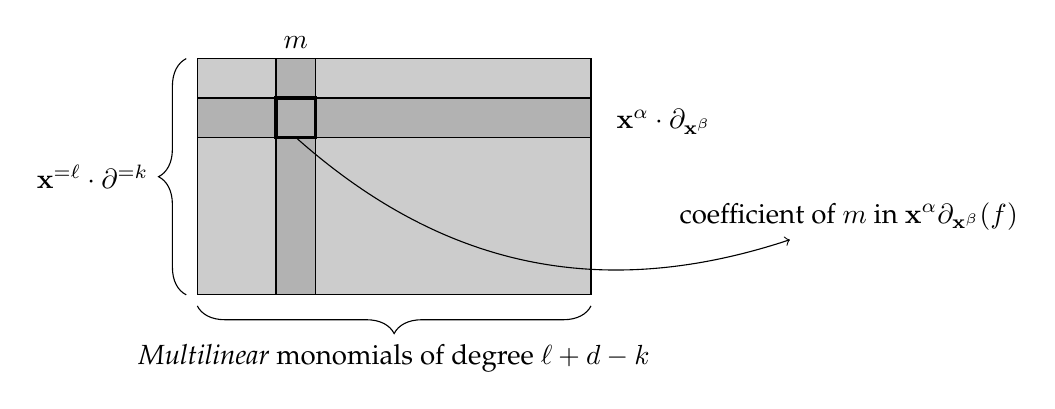
\begin{tikzpicture}
\draw[fill=black!20] (0,0) rectangle (5,3);

\draw[decorate,decoration={brace,amplitude=10pt,raise=4pt},yshift=0pt]
(0,0) -- (0,3);
\node[anchor=east] at (-0.5,1.5) {$\vecx^{=\ell} \cdot \partial^{=k}$};
\draw[decorate,decoration={brace,amplitude=10pt,mirror, raise=4pt},yshift=0pt] 
(0,0) -- (5,0);
\node[anchor=north] at (2.5,-0.5) {\emph{Multilinear} monomials of degree $\ell + d - k$};

\draw[fill=black!30] (1,0) rectangle (1.5,3);
\node at (1.25,3.2) {$m$};

\draw[fill=black!30] (0,2) rectangle (5,2.5);
\node[anchor=west] at (5.2,2.2) {$\vecx^{\alpha} \cdot \partial_{\vecx^\beta}$};

\draw[very thick] (1,2) rectangle (1.5,2.5);

\node[anchor=west] at (6,1) {coefficient of $m$ in $\vecx^\alpha \partial_{\vecx^\beta}(f)$}
edge[<-,bend left] (1.25,2);
\end{tikzpicture}


The works of \cite{KLSS,KS14} use this measure to prove a lower bound for ``\emph{low-support} depth $4$ circuits''. 
As sketched earlier, the task of proving lower bounds for general homogeneous depth $4$ circuits can be reduced to the \emph{low-support} depth $4$ circuits via random restrictions. 

\section{Reducing to `low-support' depth $4$ circuits}\label{sec:red-to-low-support}

We have already seen a sketch of how this can be done via a random restriction but let us formalize this as a lemma. 

\begin{lemma}\label{lem:red-to-low-supp}
Let $P$ be an $n$-variate degree $d$ polynomial computed by a homogeneous depth $4$ circuit $C$ of size $s \leq n^{c\sqrt{d}}$, for some $c>0$. 
Let $\rho$ be a random restriction that sets each variable to zero independently with probability $1 - 1/n^{2c}$. 
Then with probability at least $(1 - 1/s)$, the polynomial $\rho(P)$ is computed by a homogeneous depth $4$ circuit $C'$ with bottom support at most $\sqrt{d}$ and size at most $s$. 
\end{lemma}
\begin{proof}
Let $\inbrace{m_1,\dots, m_r}$ be the set of all monomials computed at the lowest layer of the depth $4$ circuit $C$ that are divisible by more than $\sqrt{d}$ distinct variables. 
Since the size of $C$ is at most $s$, we also have that $r\leq s$. 
Then,
\begin{eqnarray*}
\forall i\in [r] \qquad \Pr[\rho(m_i) \neq 0] & \leq & \frac{1}{n^{2c\sqrt{d}}}\\
\implies \qquad \Pr[\exists i \;:\; \rho(m_i) \neq 0] & \leq & \frac{r}{n^{2c\sqrt{d}}} \leq \frac{1}{n^{c\sqrt{d}}} \leq \frac{1}{s}
\end{eqnarray*}
Thus, with probability at least $(1 - 1/s)$, all the large support monomials are killed and $C$ reduces to a homogeneous depth $4$ circuit of bottom support at most $\sqrt{d}$. 
\end{proof}

\subsection{Handling random restrictions}

The previous section outlined how in essence, it would suffice to try and find an explicit polynomial for which we can prove a good enough lower bound for bounded bottom-support depth $4$ circuits. 
Let us say that we have found an explicit polynomial $g$ that requires depth $4$ circuits of size at least $n^{\sqrt{d}/100}$. 
Are we done? Let us write things down formally to see exactly what we need. 

Say the polynomial we wish to show requires large homogeneous depth $4$ circuits is $f$. 
Let us assume on the contrary that $f$ can be computed by homogeneous depth $4$ circuits of size $s < n^{\sqrt{d}/10000}$. 
Then, by \autoref{lem:red-to-low-supp}, $\rho(f)$ can be computed by a homogeneous depth $4$ circuits of bottom support bounded by $\sqrt{d}/1000$ of size $s$. 
We want to be able to say that this is a contradiction. 
We might be able to say that if $\rho(f)$ has $g$ as \emph{a projection}, that is, but setting more variables to zero in $\rho(f)$ we obtain $g$. 

Both the results of \cite{KLSS} and \cite{KS14} proceed by showing that the polynomial $g$, for which they show a lower bound for bounded bottom support circuits, is robust enough to yield the lower bound even after random restriction. 
The calculations become trickier because the calculations of $\Gamma^{[\mathrm{PSD}]}_{k,\ell}(\rho(f))$. 
However, in this survey we shall use an easier approach to generically lift any $g$ to a different polynomial $f$ such that $\rho(f)$ has $g$ as a projection. 
This trick came up during discussions with Mrinal Kumar. 

\begin{lemma}\label{lem:lin-transform-trick}
Let $\rho$ be a random restriction that sets each variable to zero independently with probability $1 - p$. 
For any polynomial $f(y_1,\dots y_n)$, define $f \circ \mathrm{Lin}_p$ as
\[
f \circ \mathrm{Lin}_p \spaced{=} f\inparen{\sum_{i=1}^t y_{1i}, \cdots, \sum_{i=1}^t y_{nt}}\quad \text{where $t = \inparen{\frac{1}{p}} n \log n$}
\]
Then, $\rho(f \circ \mathrm{Lin}_p)$ has $f$ as a projection with probability $1 - 1/2^{n}$. 
\end{lemma}
\begin{proof} For any $i = 1, \dots, n$
\begin{eqnarray*}
\quad \Pr[\rho(y_{i1}) = \dots \rho(y_{it}) = 0 ] & = & \inparen{1 - p}^t\\ 
& = & \frac{1}{n\cdot 2^n}\\
\implies \Pr[\exists i\;:\;\rho(y_{i1}) = \dots \rho(y_{it}) = 0 ]  & \leq  & \frac{1}{2^n} 
\end{eqnarray*}
Hence, with probability at least $1 - 1/2^n$, for each $i$ there is some $j$ such that $\rho(y_{ij}) \neq 0$. 
Therefore, with probability at least $1 - 1/2^n$, the polynomial $f$ is a projection of $\rho(f \circ \mathrm{Lin}_p)$. \end{proof}

In all the applications, as in \autoref{lem:red-to-low-supp}, we would have $p = 1/n^{O(1)}$. 
Thus, we would only incur a polynomial blow-up in the number of variables from $f$ to $f\circ \mathrm{Lin}_p$. 
Hence, we can focus on proving a lower bound  a homogeneous depth $4$ circuit of bottom support at most $r$ (which would eventually be something like $\sqrt{d}/100$). 

\begin{lemma}[\cite{KLSS}]\label{lem:upper-bound-low-supp}
Let $P$ be an $n$-variate degree $d$ polynomial computed by a homogeneous depth $4$ circuit of size $s$ and bottom-support at most $r$. 
Then for any $k,\ell$ such that $\ell + rk \leq n/2$, 
\[
\Gamma^{\mathrm{PSD}}_{k,\ell}(P) \quad \leq \quad s \cdot \binom{\frac{2d}{r}+k}{k}\cdot \binom{n}{\ell+rk}. 
\]
\end{lemma}

The proof of this lemma is exactly along the description in of Intuition - (2): split the circuit into multiquadratic and non-multiquadratic part, and show that the non-multiquadratic part contributes no multilinear monomials. 
But to just put things in perspective, we shall be dealing with parameters $r = \sqrt{d}/100$, $k = \sqrt{d}$ and $\ell = \frac{n}{2}(1 - \epsilon)$ for $\epsilon = O\inparen{\frac{\log d}{\sqrt{d}}}$. 
The above bound, by \autoref{lem:binom-approx}, can be seen to reduce to
\[
\Gamma^{\mathrm{PSD}}_{k,\ell}(P) \quad \leq \quad s \cdot \binom{n}{\ell} \cdot (1+\epsilon)^{2rk} \cdot 2^{O(\sqrt{d})}
\]


\subsection*{Sanity checks}

Let us first check if this measure can at least in principle yield a lower bound for us. 
The best way to do this is to get some heuristic estimate of what we expect the measure to be for a random $n$-variate degree $d$ polynomial $R$. \\

{\bf Heuristic Estimate. } For a random $n$-variate degree $d$ polynomial $R$, we expect the $\Gamma^{\mathrm{PSD}}_{k,\ell}(R)$ to be as large as it can be, i.e.
\[
\Gamma^{\mathrm{PSD}}_{k,\ell}(R) \spaced{\approx} \min\inparen{\binom{n}{k}\cdot \binom{n}{\ell}, \binom{n}{\ell + d-k}}
\]

As a first step, one should first check that if we could indeed find a polynomial $P$ for which the bound is as large as stated above, do we get a useful lower bound from \autoref{lem:upper-bound-low-supp}? Turns out that if we were to choose our parameters carefully, we do indeed get the lower bound. 
Just to give a sense of how \emph{careful} we need to be, here is some of the parameters that are chosen in \cite{KLSS,KS14}. 

\begin{itemize}
\item The number of variables $n$ is at least the cube of the degree $d$. 
\item The model we shall be working with is bottom-support $r$ where $r = \sqrt{d}/1000$. 
\item The order of derivatives $k = \sqrt{d}$. 
\item The degree of the shift $\ell$ shall be chosen as $\ell = \frac{n}{2}\inparen{1 - \epsilon}$ where $\epsilon = \frac{\log d}{c\sqrt{d}}$ for a suitable constant $c$. 
\end{itemize}

The above choice of parameters might already seem pretty fragile but these are not the most delicate choices! 
While proving the lower bound on $\Gamma^{\mathrm{PSD}}_{k,\ell}$ for an explicit polynomial, the number of monomials etc. need to be tailored to perfection to make the proof work. 

\section{The surrogate rank approach of \cite{KLSS}}

The goal is now to find an explicit polynomial $P$ such that $\mathrm{PSD}_{k,\ell}(P)$ has large rank. 
One way to prove that a set of polynomials are linearly independent is to show that they have distinct leading monomials (as used \cite{gkks13} etc.) Another method is to show that these polynomials are \emph{almost orthogonal}. 
An example of this phenomenon can be seen in the following fact. 

\begin{fact}
Let $M$ be a square matrix such that the absolute value of the diagonal entry is larger than sum of the absolute values of the non-diagonal entries in that row or column, i.e. $\abs{M_{ii}} \geq \sum_{j\neq i} \abs{M_{ij}}$ for all $i$. 
Then the matrix $M$ is full rank. 
\end{fact}

Such matrices are also called \emph{diagonally dominant matrices}, and captures the notion of \emph{almost orthogonal} vectors alluded to earlier. 
For symmetric matrices $M$, the following bound of Alon~\cite{Alo09}.

\begin{lemma}[\cite{Alo09}]\label{lem:trace-bound} For any real symmetric matrix $M$, 
\[
\rank(M) \spaced{\geq} \frac{(\mathrm{Tr}(M))^2}{\mathrm{Tr}(M^2)}
\]
\end{lemma}

We'll see the proof of this shortly but it would shed some more intuition to see what the above lemma yields for a diagonally dominant matrix. 
Let $M$ be a matrix of the form
\[
M \spaced{=} \insquare{\begin{array}{cccc}
D &  d & \dots &  d\\
 d & D & \dots & d\\
\vdots & \vdots & \ddots & \vdots \\
d & d & \dots & D
\end{array}}_{r \times r}
\]
Then, $\mathrm{Tr}(M) = D\cdot r$, and $\mathrm{Tr}(M^2) = (D^2 + (r-1)d^2)r = O(D^2 r + r^2 d^2)$. 
If $D > (r-1)d^2$, then $\mathrm{Tr}(M^2) = O(D^2r)$. 
Thus, the above lemma gives that $\rank(M) = \Omega(r)$. 
\begin{proof}
By the spectral theorem, any real symmetric matrix has a basis of eigen vectors with eigenvalues $\lambda_1,\dots, \lambda_n$ where $n$ is the dimension of the matrix. 
If $\lambda_1,\dots, \lambda_r$ are the non-zero eigenvalues, then 
\begin{eqnarray*}
\mathrm{Tr}(M) &   =  & \sum_{i=1}^r \lambda_i\\
& \leq & \sqrt{r} \;\cdot \; \inparen{\sum_{i=1}^r \lambda_i^2} = \sqrt{r}\;\cdot \; \mathrm{Tr}(M^2)\\
\implies r & \geq & \frac{(\mathrm{Tr}(M))^2}{\mathrm{Tr}(M^2)}
\end{eqnarray*}
\end{proof}

The bound of \cite{KLSS} for an explicit polynomial $P$ proceeds by considering the matrix $B$ where each row is indexed by a pair of multilinear monomials $(m_1,m_2)$  of degree $k$ and $\ell$ respectively, and the row is just the coefficients of the monomials of $\mathrm{mult}(m_2 \partial_{m_1}(P))$ in a fixed order. 
Note that $B$ is not even a square matrix, and certainly not symmetric. 
However, the matrix $M = B B^T$ is a symmetric square matrix such that $\rank(M) \leq \rank(B)$. \\

Let us spend some time understand the entries of $M$. 
The $(i,j)$-th entry of $M$ is precisely the inner-product of row $i$ and row $j$ of $B$. 
If $P$ is a polynomial with just zero-one coefficients, then the $i$-th diagonal entry is precisely the number of non-zero entries in row $i$ of $B$. 
Thus,
\begin{eqnarray*}
\mathrm{Tr}(M) & = & \text{number of non-zero entries in $B$}\\
  & = & \text{(\# cols of $B$)} \cdot \mathop{\mathbb{E}}_i[\text{\# non-zero entries in $i$-th col of $B$}] 
\end{eqnarray*}
The calculation for $\mathrm{Tr}(M^2)$ requires a little more care. 
Let $M_i$ refer to the $i$-th row of $M$ and $B_i$ refer to the $i$-th row of $B$. 
Then,
\begin{eqnarray*}
\mathrm{Tr}(M^2) & = & \sum_{i} \inangle{M_i, M_i}\\
 & = & \sum_{i} \sum_j \inangle{B_i, B_j}^2 \spaced{=}\sum_{i} \sum_j \inparen{\sum_m B_{im} B_{jm}}^2\\
 & = & \sum_{i} \sum_j \sum_m B_{im}^2 B_{jm}^2  \spaced{+} \sum_i \sum_j \sum_{m\neq m'} B_{im}B_{im'}B_{jm}B_{jm'}\\
 & = & \sum_{m} \inparen{\sum_i \sum_j B_{im} B_{jm}}  \spaced{+} \sum_i \sum_j \sum_{m\neq m'} B_{im}B_{im'}B_{jm}B_{jm'}\\
 & = & \quad\quad\quad T_1 \quad\quad\quad\quad\quad\quad + \quad\quad\quad\quad\quad\quad T_2
\end{eqnarray*}
The first term $T_1$ is easy to calculate:
\begin{eqnarray*}
T_1 & = & \text{(\# cols of $B$)} \cdot \mathop{\mathbb{E}}_i[\inparen{\text{\# non-zero entries in $i$-th col of $B$}}^2] \\
 & \stackrel{\tiny \text{(hopefully)}}{\approx} & \text{(\# cols of $B$)} \cdot \mathop{\mathbb{E}}_i[\inparen{\text{\# non-zero entries in $i$-th col of $B$}}]^2
\end{eqnarray*}
The term $T_2$ roughly corresponds to the number of $2\times 2$ submatrices of $B$ that is $\insquare{\begin{array}{cc}1 & 1 \\ 1 & 1\end{array}}$. 
If we could somehow show that there are not too many such submatrices, then $\mathrm{Tr}(M^2)$ is essentially dominated by $T_1$. 
That would then yield that $\rank(M) \gtrapprox \text{(\# cols of $B$)}$. 

\subsection*{Obtaining a bound on $T_2$:}

\[
T_2 \spaced{=} \sum_i \sum_j \sum_{m\neq m'} B_{im}B_{im'}B_{jm}B_{jm'}
\]
Each term $B_{im}B_{im'}B_{jm}B_{jm'}$ that is non-zero corresponds to a $2\times 2$ submatrix of $B$ (indexed by rows $i,j$ and columns $m,m'$) that is $\insquare{\begin{array}{cc} 1 & 1\\ 1&1
  \end{array}}$. \\

The columns of $B$ are indexed by multilinear monomials of degree $\ell + d - k$, and the rows of $B$ are indexed by a derivative and a shift. 
Let row $i$ correspond to $\mathrm{mult}(\gamma_1 \cdot \partial_{\alpha_1}(P))$ and row $j$ to $\mathrm{mult}(\gamma_1 \cdot \partial_{\alpha_1}(P))$. 
Thus, if the $2\times 2$ minor indexed by rows $i,j$ and columns $m,m'$ equals $\insquare{\begin{array}{cc} 1 & 1\\ 1&1 \end{array}}$, then there exists $\beta_1, \beta_2,\beta_3,\beta_4 \in P$ such that
\begin{eqnarray*}
m \spaced{=} \frac{\beta_1}{\alpha_1}\cdot \gamma_1 & = & \frac{\beta_3}{\alpha_2} \cdot  \gamma_2\\
m' \spaced{=} \frac{\beta_2}{\alpha_1}\cdot \gamma_1 & = & \frac{\beta_4}{\alpha_2}\cdot \gamma_2\\
\implies \frac{\beta_1}{\beta_3} & = & \frac{\beta_2}{\beta_4}
\end{eqnarray*}
Following notation used in \cite{KLSS}, we shall call $\beta_1,\beta_2,\beta_3,\beta_4$ as the \emph{label} of the $2\times 2$ minor. 
Since $m\neq m'$, we also have that $\beta_1 \neq \beta_2$. 
What we'd like to say that the only way $\beta_1/\beta_3 = \beta_2/\beta_4$ is if $\beta_3 = \beta_1$ and $\beta_2 = \beta_4$. 
This need not be true in general of course, but this is where the choice of the polynomial comes in. 

\begin{claim}
If $P$ is the $\NW_{d,d^3, e}$ polynomial for $e = \frac{d}{3}$ then any $2\times 2$ minor of $B$ (with the order of derivatives $k = o(d)$) that is $\insquare{\begin{array}{cc} 1&1\\1&1\end{array}}$ has label $\beta_1,\beta_2,\beta_3,\beta_4$ where $\beta_1 = \beta_3$ and $\beta_2 = \beta_4$, or $\beta_1 = \beta_2$ and $\beta_3 = \beta_4$. 
\end{claim}
\begin{proof}
Assume that $\beta_1 \neq \beta_3$. 
Then by \autoref{lem:NW-low-intersection} we know that they differ in at least $2d/3$ places. 
But then, $\beta_1/\beta_3 = \beta_2/\beta_4$ forces that $\beta_1$ and $\beta_3$ must agree at least $2d/3$ places forcing $\beta_1 = \beta_2$. 
\end{proof}

Thus, for the $\NW$-polynomial the number of such boxes is quite small. 
Using this, albeit with a reasonable amount of sweat, one can estimate $T_2$ to show that $T_2 = O(T_1)$. 
Thus, \cite{KLSS} obtain the following bound. 

\begin{lemma}[\cite{KLSS}]
For the polynomial $\NW_{d,d^3,e}$, for $e = \frac{d}{3}$, and $k = \sqrt{d}$ and $\ell = \frac{n}{2}\inparen{1 - \frac{\log d}{\sqrt{d}}}$ we have the bound
\[
\Gamma^{\mathrm{PSD}}_{k,\ell}(\NW_{d,d^3,e}) \spaced{\geq} \frac{1}{\poly(n,d)} \cdot \min\inparen{\binom{n}{\ell + d - k}, \binom{d}{k}^2 \cdot d^k \cdot k! \cdot \binom{n}{\ell}}
\]
\end{lemma}
Note that the first term of the $\min$ in the RHS is the number of columns of $B$, as we had heuristically estimated. 
Simplifying the RHS using \autoref{lem:binom-approx}, we get
\[
\Gamma^{\mathrm{PSD}}_{k,\ell}(\NW_{d,d^3,e}) \spaced{\geq} \frac{1}{\poly(n,d)} \cdot \binom{n}{\ell}\cdot \exp\inparen{c\cdot \epsilon (d - k)}
\]
for some constant $c > 0$. 
Since $\epsilon = \frac{\log d}{\sqrt{d}}$, we get 
\[
\Gamma^{\mathrm{PSD}}_{k,\ell}(\NW_{d,d^3,e}) \spaced{\geq} \frac{1}{\poly(n,d)} \cdot \binom{n}{\ell}\cdot \exp\inparen{c\cdot \sqrt{d}\cdot \log d}
\]
With the above bound and \autoref{lem:upper-bound-low-supp}, we get the lower bound of \cite{KLSS}. 
\begin{theorem}[\cite{KLSS}]\label{thm:KLSS-lowsupp}
Any depth $4$ homogeneous circuit of bottom support $r = \sqrt{d}/1000$ computing the polynomial $\NW_{d,d^3,d/3}$ over a characteristic zero field must have top fan-in $s = d^{\Omega(\sqrt{d})}$. 

In fact, more generally, any homogeneous depth $4$ circuit of bottom support bounded by $r$ computing $\NW_{d,m,e}$ for suitably chosen parameters must have top fanin $s = d^{\Omega(d/r)}$. 
\end{theorem}

Coupling with \autoref{lem:lin-transform-trick}, we obtain (a slight reformulation of) their main theorem. 

\begin{theorem}[\cite{KLSS}]\label{thm:KLSS-main}
Any depth $4$ homogeneous computing the polynomial $\NW_{d,d^3,d/3}\circ \mathrm{Lin}$ over a characteristic zero field must have size $s = d^{\Omega(\sqrt{d})}$. 
\end{theorem}

\section{The leading monomial approach of \cite{KS14}}

Shortly after \cite{KLSS}, a purely combinatorial proof of the result was presented by Kumar and Saraf~\cite{KS14}. 
More over, they were able to prove the lower bound of $n^{\Omega(\sqrt{d})}$ for the size of any homogeneous depth $4$ circuit computing $\IMM_{n,d}$ (for some suitable choices of $n$ and $d$). 
This was a strengthening of \cite{KLSS} in two ways -- (1) it worked over any field, and (2) the lower bound was for a polynomial that we know can be computed small arithmetic circuit. 

The calculations of \cite{KS14} are much more trickier than \cite{KLSS} but there are quite a few interesting ideas that would even have application in other areas. \\

The earlier lower bounds of \cite{gkks13,KSS13,FLMS13} required a lower bound on the dimension of shifted partial derivatives of a polynomial $P$, and this was obtained by finding a \emph{large} set of \emph{distinct leading monomials}. 
In \cite{KS14}, they take this approach but require a very careful analysis. 
The key difference in this setting is the following: 

\begin{quote}
  If $\beta$ is the leading monomial of a polynomial $P$, then for any monomial $\gamma$, we also have that $\beta \cdot \gamma$ is the leading monomial of $\gamma P$. 

  However, the leading monomial of $\mathrm{mult}(\gamma P)$ could be $\beta' \cdot \gamma$ for some $\beta' \neq \beta$ (as higher monomials could be made non-multilinear during the shift by $\gamma$). 
\end{quote}

The multilinear projection makes the task of counting leading monomials much harder and \cite{KS14} come up with a clever method to estimate this. 

\subsection*{Leading monomials after multilinear projections}

Let $P$ the polynomial for which we are trying to lower bound $\Gamma^{\mathrm{PSD}}_{k,\ell}(P)$. 
For every monomial multilinear monomial $\alpha$ of degree $k$, and a monomial $\beta \in \partial_\alpha(P)$, define the set $A(\alpha, \beta)$ as
\[
A(\alpha, \beta) \spaced{=} \setdef{\gamma}{\begin{array}{c}\deg(\gamma) = \ell + d - k\;\text{and there is a $\gamma'$ of degree $\ell$}\\\text{such that }\gamma  = \mathrm{LM}(\mathrm{mult}(\gamma' \cdot \partial_\alpha(P))) = \gamma' \cdot \beta \end{array}}
\]
In other words, we want the number of distinct monomials that are contributed by $\beta$, which are also distinct leading monomials obtained from $\partial_\alpha(P)$ that are divisible by $\beta$. 
We then have
\begin{equation}\label{eqn:union-of-As}
\Gamma^{\mathrm{PSD}}_{k,\ell}(P) \spaced{\geq} \abs{\Union_{\alpha, \beta} A(\alpha, \beta)}
\end{equation}

\noindent
{\bf Choice of derivatives:} Instead of looking at all derivatives in  $\partial^{=k}$, we shall restrict ourselves to just a subset of derivatives. Restricting the above union to a subset $\Delta  \subset \vecx^{=k}$ still continues to remain a lower bound for $\Gamma^{\mathrm{PSD}}_{k,\ell}(P)$. Keeping in mind that we are dealing with $P = \NW_{d,m,e}$ we shall choose $\Delta$ to be a set of monomials of the form $x_{1a_1}\cdots x_{ka_k}$ with each $a_i \leq m$ so as to have $m^k$ derivatives in total. This shall become relevant later. 
\begin{equation}\label{eqn:union-of-As}
\Gamma^{\mathrm{PSD}}_{k,\ell}(P) \spaced{\geq} \abs{\Union_{\substack{\alpha \in \Delta \\\beta \in \vecx^{=\ell}}} A(\alpha, \beta)}
\end{equation}

The standard technique to obtain a lower bound on the union of sets is via the \emph{Inclusion-Exclusion} principle. 

\begin{lemma}[Inclusion-Exclusion Principle]\label{lem:inc-exc}
For any collection of sets $A_1,\dots, A_r$,
\[
\abs{\Union_i A_i} \spaced{\geq} \sum_{i} \abs{A_i} \spaced{-} \sum_{i\neq j}\abs{A_i\intersection A_j}
\]
\end{lemma}

If we were to somehow show that $\sum_{i\neq j}\abs{A_i\intersection A_j} \leq \frac{1}{2}\sum_i \abs{A_i}$, then we obtain that $\abs{\union_i A_i} \geq \frac{1}{2}\cdot \sum_i \abs{A_i}$. 
This is what shall be employed for the sets $A(\alpha, \beta)$, except that we quickly run into two immediate problems. 

\begin{enumerate}
  \item How do we even estimate $A(\alpha, \beta)$? The set of $\gamma'$ such that $\gamma' \beta = \mathrm{LM}(\partial_\alpha(P))$ do not seem to have any nice combinatorial structure. 
  \item What if it so happens that $\sum \abs{A(\alpha_1,\beta_1)\intersection A(\alpha_2,\beta_2)} = 100 \sum \abs{A(\alpha,\beta)}$? Inclusion-Exclusion does not yield anything in that case. 
\end{enumerate}


It so turns out that the second point actually is the case. 
In fact for $\IMM_{n,d}$, the second term turns out to be greater than the first term by a factor of $n^{\sqrt{d}/1000}$ or so! 
In \cite{KS14}, they prove a wonderful strengthened version of the Inclusion-Exclusion principle which allows them to handle the second hurdle. 

\begin{lemma}[Stronger Inclusion-Exclusion \cite{KS14}]\label{lem:str-inc-exc}
Let $A_1,\dots, A_r$ be sets such that there is some $\lambda > 1$ such that
\[
\sum_{i\neq j} \abs{A_i \intersection A_j} \spaced{\leq} \sum_i \lambda \cdot \abs{A_i}
\]
Then, 
\[
\abs{\Union_i A_i} \spaced{\geq} \inparen{\frac{1}{4\lambda}} \cdot \inparen{\sum_i \abs{A_i}}
\]
\end{lemma}

In other words, as long as the second term of the Inclusion-Exclusion principle is \emph{not too much larger} than the first term, we still can get non-trivial bounds on the union. 

\begin{proof}
Let $p = \frac{1}{2\lambda} < 1$. 
Define sets $A_1',\dots, A_r'$ such that $A_i' \subseteq A_i$ obtained by adding each element of $A_i$ to $A_i'$ independently with probability $p$. 
Since $A_i' \subseteq A_i$, we also have that $\abs{\union A_i} \geq \abs{\union  A_i'}$. 
By linearity of expectation, 
\[
\E\insquare{\sum_i \abs{A_i'}} \spaced{=} p \sum_{i} \abs{A_i} 
\]
More importantly, by the sampling process,
\[
\E\insquare{\abs{A_i' \intersection A_j'}} \spaced{=} p^2 \cdot \abs{A_i \intersection A_j}
\]
as any common element must be added to both $A_i'$ \emph{and} $A_j'$, and either of these events happen independently with probability $p$ each. 
Since $\sum_{i,j}\abs{A_i' \intersection A_j'}$ drops by a factor of $p^2$, we are now in a position to apply the \autoref{lem:inc-exc} to the $A_i'$s. 
\begin{eqnarray*}
\abs{\Union A_i} & \geq &  \E\insquare{\abs{\Union A_i'}}\\
& \geq & \E\insquare{\sum_i \abs{A_i'}} \spaced{-} \E\insquare{\abs{A_i' \intersection A_j'}}\\
& = & p \inparen{\sum_i \abs{A_i}} \spaced{-} p^2\inparen{\sum_{i\neq j}\abs{A_i \intersection A_j}}\\
& \geq & p \inparen{\sum_i \abs{A_i}} \spaced{-} p^2 \lambda \inparen{\sum_i \abs{A_i}}\\
& \geq & \frac{p}{2} \inparen{\sum_i \abs{A_i}} \spaced{=} \frac{1}{4\lambda} \inparen{\sum_i \abs{A_i}}
\end{eqnarray*}
\end{proof}

\begin{corollary}\label{cor:inc-exc-str}
Considers sets $A_1,\dots, A_r$  and let $S_1 = \sum_i \abs{A_i}$ and $S_2 = \sum_{i\neq j} \abs{A_i \intersection A_j}$. 
Then, 
\[
\abs{\Union A_i} \spaced{\geq} \frac{S_1}{4} \cdot \min\inparen{1,\frac{S_1}{S_2}}
\]
\end{corollary}

We can now proceed to lower bound $\abs{\Union A(\alpha, \beta)}$ via inclusion exclusion.

\subsection*{Estimating $\abs{\Union A(\alpha, \beta)}$ via Inclusion-Exclusion}
\[
\abs{\Union_{\alpha, \beta}A(\alpha,\beta)}\spaced{\geq} \sum_{\alpha,\beta}\abs{A(\alpha, \beta)} \spaced{-} \sum_{(\alpha, \beta)\neq (\alpha',\beta')}\abs{A(\alpha, \beta) \intersection A(\alpha',\beta')}
\]

Let us first address the term $\sum \abs{A(\alpha, \beta)}$. 
As mentioned earlier, it is not an easy task to get a good handle on the set $A(\alpha, \beta)$ for polynomial such as $\NW$ or $\IMM$, for any reasonable monomial ordering. 
However, \cite{KS14} circumvent this difficult by using an indirect approach to estimate this term. 

For any derivative $\alpha$ and $\beta \in \partial_\alpha(P)$, define the set $S(\alpha, \beta)$ as the following set of multilinear monomials of degree $\ell$ that is disjoint from $\beta$. 
\[
S(\alpha, \beta) \spaced{=} \setdef{\gamma}{\begin{array}{c}\text{$\gamma$ is multilinear, has}\\\text{degree $\ell$ and $\gcd(\beta,\gamma)=1$ }\end{array}}
\]
This on the other hand is independent of any monomial ordering, and is also easy to calculate:
\[
\text{For every $\alpha, \beta$}\quad\quad \abs{S(\alpha, \beta)} \spaced{=} \binom{n - d + k}{\ell}.
\] 
\begin{lemma}[\cite{KS14}]\label{lem:As-to-Ss}
For any $\alpha$, 
\[
\sum_{\beta} \abs{A(\alpha, \beta)} \spaced{\geq} \abs{\Union_{\beta} S(\alpha, \beta)}
\]
\end{lemma}
\begin{proof}
Consider any $\gamma \in \Union_{\beta}S(\alpha, \beta)$. 
By definition, there is at least one non-multilinear monomial in $\gamma \cdot \partial_\alpha(P)$. 
Thus, in particular $\mathrm{LM}(\mathrm{mult}(\gamma \cdot \partial_\alpha(P))$ is non-zero and equal to some $\gamma \cdot \beta$ for some monomial $\beta \in \partial_\alpha(P)$. 
This also implies that $\gamma' = \gamma\cdot \beta \in A(\alpha, \beta)$. 
This yields an injective map $\phi$ 
\[
\phi:\Union_\beta S(\alpha,\beta) \spaced{\rightarrowtail} \setdef{(\beta, \gamma')}{\beta\in \partial_\alpha(P)\;,\;\gamma' \in A(\alpha, \beta)}
\] 
Since the size of the RHS is precisely $\sum_\beta \abs{A(\alpha, \beta)}$, the lemma follows. 
\end{proof}

Thus, by another use of Inclusion-Exclusion on the $S(\alpha, \beta)$'s, we get
\begin{eqnarray*}
\abs{\Union_{\alpha, \beta}A(\alpha,\beta)}&\geq& \sum_{\alpha,\beta}\abs{A(\alpha, \beta)} \spaced{-} \sum_{(\alpha, \beta)\neq (\alpha',\beta')}\abs{A(\alpha, \beta) \intersection A(\alpha',\beta')}\\
 & \geq & \sum_\alpha \inparen{\sum_\beta \abs{S(\alpha, \beta)}} \spaced{-} \sum_\alpha \inparen{\sum_{\beta \neq \beta'}\abs{S(\alpha, \beta)\intersection S(\alpha,\beta')}}\\
 & & \quad\quad \spaced{-} \sum_{(\alpha, \beta)\neq (\alpha',\beta')}\abs{A(\alpha, \beta) \intersection A(\alpha',\beta')}
\end{eqnarray*}
Let us call the three terms in the RHS of the last equation as $T_1$, $T_2$ and $T_3$ respectively. 
Since we know the size of each $S(\alpha, \beta)$ exactly, the value of $T_1$ is easily obtained. 
\begin{lemma}[\cite{KS14}]\label{lem:T_1-value}
\begin{eqnarray*}
T_1(\alpha) \spaced{:=} \sum_{\beta}\abs{S(\alpha,\beta)}&=&\text{(\# mons in a deriv)} \cdot \binom{n-d+k}{\ell}
\end{eqnarray*}
\end{lemma}

\noindent
We shall be simplifying such binomial coefficients very often so let us recall the \autoref{lem:binom-approx}. 

\binomapprox*

\noindent
Since our of parameters would be $\epsilon = \Theta\inparen{\frac{\log d}{\sqrt{d}}}$, the bound on $T_1$ can be simplified as
\begin{eqnarray*}
T_1(\alpha)  & =  &\text{(\# mons in a deriv)} \cdot \binom{n}{\ell} \cdot \inparen{\frac{1+\epsilon}{2}}^{d-k} \cdot \exp(O(\log^2 d))\\
& = & m^{e-k}\cdot \binom{n}{\ell} \cdot \inparen{\frac{1+\epsilon}{2}}^{d-k} \cdot \exp(O(\log^2 d))
\end{eqnarray*}
\begin{remark*}To avoid writing this factor of $\exp(O(\log^2 d))$, we shall use $\approx$ of $\gtrsim$ or $\lesssim$ to indicate that a factor $\exp(O(\log^2 d))$ is omitted. 
\end{remark*}

\bigskip

So far we have not used any property of the polynomial $P$. 
But this becomes crucial in the calculation of $T_2$ and $T_3$. 
To get a sense of how these calculations proceed in \cite{KS14}, we present the full calculation for the case of $P = \NW_{d,m,e}$ for suitable choices of the parameters $m,d,e$. 
\begin{lemma}[\cite{KS14}]\label{lem:T_2-for-NW}
For the polynomial $\NW_{d,m,e}$, if $n = md$ and $\ell = \frac{n}{2}(1 - \epsilon)$ for $\epsilon = \Theta\inparen{\frac{\log d}{\sqrt{d}}}$, for every $\alpha \in \Delta$, 
\[
T_2(\alpha)\spaced{:=} \sum_{\beta\neq \beta'}\abs{S(\alpha, \beta)\intersection S(\alpha, \beta')} \quad \lesssim \quad m^{2(e-k)}\cdot \binom{n}{\ell} \cdot \inparen{\frac{1+\epsilon}{2}}^{2d -2k} 
\]
\end{lemma}
\begin{proof}
Recall that $S(\alpha,\beta) \intersection S(\alpha,\beta')$ is just set of all multilinear monomials $\gamma$ of degree $\ell$ that are disjoint from both $\beta$ and $\beta'$.
Hence, for any pair of multilinear degree $(d-k)$ monomials $\beta \neq \beta' \in \partial_\alpha(P)$ such that $\deg(\gcd(\beta, \beta')) = t$, we know that 
\[
\abs{S(\alpha, \beta)\intersection S(\alpha, \beta')} \spaced{=} \binom{n - 2d + 2k +t}{\ell}
\]
Thus, if we can count the number of pairs $(\beta, \beta')$ that agree on exactly $t$ places, we can obtain $T_2(\alpha)$. 
Note that for $\NW_{d,m,e}$, any two $\beta, \beta' \in\partial_\alpha(\NW_{d,m,e})$ can agree on at most $e-k$ places. 
Further, the number of pairs that agree in exactly $0\leq t\leq e-k$ places is at most
\[
m^{e-k} \cdot \binom{d-k}{t} \cdot (m-1)^{e-k-t}
\]
as there are $m^{e-k}$ choices for $\beta$, and $\binom{d-k}{t}$ choices for places where they may agree, and $(m-1)^{e-k-t}$ choices for $\beta'$ that agree with $\beta$ on those $t$ places. 
Thus,
\begin{eqnarray*}
T_2(\alpha) &\leq& \sum_{t=0}^{e-k} m^{e-k} \cdot \binom{d-k}{t} \cdot (m-1)^{e-k-t} \cdot  \binom{n - 2d + 2k +t}{\ell}\\
& \approx  & \sum_{t=0}^{e-k} m^{e-k} \cdot \binom{d-k}{t} \cdot (m-1)^{e-k-t} \cdot  \binom{n}{\ell} \frac{1}{2^{2d-2k -t}}\cdot (1+\epsilon)^{2d - 2k - t}\\
& \leq & m^{2(e-k)}\binom{n}{\ell}\inparen{\frac{1+\epsilon}{2}}^{2d -2k}\cdot\sum_{t=0}^{e-k}\binom{d-k}{t}\inparen{\frac{2}{(1+\epsilon)m}}^t\\
& \leq & m^{2(e-k)}\binom{n}{\ell}\inparen{\frac{1+\epsilon}{2}}^{2d -2k}\cdot \inparen{1+\frac{2}{(1+\epsilon)m}}^{d-k}\\
& = & m^{2(e-k)}\cdot \binom{n}{\ell} \cdot \inparen{\frac{1+\epsilon}{2}}^{2d -2k}\cdot O(1) \qquad\text{if $m = \Omega(d)$}\qedhere
\end{eqnarray*}
\end{proof}
\noindent
Combining this with \autoref{lem:T_1-value} and using Inclusion-Exclusion (\autoref{cor:inc-exc-str}),
\begin{eqnarray*}
\abs{\Union_{\beta} S(\alpha,\beta)} &\spaced{\gtrsim}& T_1(\alpha) \cdot \min\inparen{1,\frac{T_1(\alpha)}{T_2(\alpha)}}\\
& \approx & T_1(\alpha) \cdot \min\inparen{1,\frac{\pfrac{2}{1+\epsilon}^{d-k}}{m^{e-k}}}
\end{eqnarray*}
To maximize this, if we choose the parameters $m,d,e$ such that $T_1(\alpha) \approx T_2(\alpha)$, we obtain the following corollary. 
\begin{corollary}\label{cor:T2-bound}
Consider the polynomial $\NW_{d,m,e}$ with $n = md$ and $m = \Omega(d)$. 
If $\ell = \frac{n}{2}(1 - \epsilon)$ for $\epsilon = \Theta\inparen{\frac{\log d}{\sqrt{d}}}$ and $e$ chosen so that
\[
m^{e-k} \quad \stackrel{\poly}{=} \quad \inparen{\frac{2}{1+\epsilon}}^{d-k}
\]
then
\[
\sum_{\substack{\alpha \in \Delta\\\beta \in \partial_\alpha(\mathrm{NW})}}\abs{A(\alpha, \beta)} \spaced{\gtrsim} \abs{\Delta}\cdot  \binom{n}{\ell}
\]
\end{corollary}
\begin{proof}
By \autoref{lem:As-to-Ss}, we know that
\[
\sum_{\substack{\alpha\in \Delta\\\beta \in \partial_\alpha(P)}} \abs{A(\alpha,\beta)} \spaced{\geq} \abs{\Delta} \cdot \abs{\Union_{\beta} S(\alpha,\beta)}.
\]
Furthermore, from the discussion above, if $T_1(\alpha) \approx T_2(\alpha)$ then
\begin{eqnarray*}
\abs{\Union_{\beta}S(\alpha, \beta)} &\gtrsim &  T_1(\alpha) \cdot \min\inparen{1,\frac{T_1(\alpha)}{T_2(\alpha)}}\\
 & = & T_1(\alpha)\\
 & \approx & \binom{n}{\ell}
\end{eqnarray*}
as $T_1(\alpha) \approx T_2(\alpha)$ forces $m^{e-k} \approx \inparen{\frac{2}{1+\epsilon}}^{d-k}$. Therefore,
\[
\sum_{\substack{\alpha\in \Delta\\\beta \in \partial_\alpha(P)}} \abs{A(\alpha,\beta)} \spaced{\gtrsim} \abs{\Delta} \cdot \binom{n}{\ell}\qedhere
\]
\end{proof}

Note that $e$ needs to tailored very precisely to force the above condition! 
If $e$ is chosen too large or small, we get nothing from this whole exercise!

In the case of $\IMM$ this calculations gets a lot messier. 
The calculation would similarly force that the number of monomials must be in a very narrow range. 
This is achieved by instead looking at a random subgraph of the generic ABP of suitable sparsity to ensure the following two properties:
\begin{itemize}
  \item The number of monomials in any derivative is exactly as demanded. 
  \item `Most' pairs of monomials $(\beta, \beta')$ agree on `few' places. 
\end{itemize}

\subsection*{Upper bounding $\sum \abs{A(\alpha,\beta)\intersection A(\alpha',\beta')}$}

We are still left with the task of upper bounding
\[
T_3 \quad = \quad \sum_{(\alpha, \beta)\neq (\alpha',\beta')} \abs{A(\alpha, \beta) \intersection A(\alpha',\beta')}
\]
As mentioned earlier, we really do not have a good handle on the set $A(\alpha, \beta)$, and certainly not on the intersection of two such sets. 
Once again, we shall use a proxy that is easier to estimate to upper bound $T_3$. 

The set $A(\alpha, \beta) \intersection A(\alpha',\beta')$ consists of multilinear monomials $\gamma$ of degree $\ell + d -k$ such that there exists multilinear monomials $\gamma', \gamma''$ of degree $\ell$ satisfying
\begin{eqnarray*}
\gamma & = & \gamma' \beta \spaced{=} \gamma'' \beta',\\
 \gamma'\beta & = & \mathrm{LM}(\mathrm{mult}(\gamma' \partial_\alpha(P)))\\
\text{and}\quad \gamma''\beta' & = & \mathrm{LM}(\mathrm{mult}(\gamma'' \partial_{\alpha'}(P)))
\end{eqnarray*}
This in particular implies that $\gamma$ must be divisible by both $\beta$ and $\beta'$. 

\begin{observation}\label{obs:T3-proxy}
If $\deg(\gcd(\beta, \beta')) = t$, then
\[
\abs{A(\alpha, \beta) \intersection A(\alpha', \beta')} \spaced{\leq} \binom{n - 2d + 2k + t}{\ell - d + k +t}
\]
\end{observation}
\begin{proof}
Every monomial $\gamma \in A(\alpha, \beta) \intersection A(\alpha', \beta')$ must be divisible by $\beta$ and $\beta'$. 
Since $\abs{\beta \union \beta'} = 2d - 2k - t$, the number of choices of $\gamma$ is precisely
\[
\binom{n - (2d - 2k -t)}{(\ell + d - k) - (2d - 2k - t)} \quad = \quad \binom{n - 2d + 2k + t}{\ell - d + k + t}\qedhere
\]
\end{proof}

One needs a similar argument as in the case of $T_2$ to figure out how many pairs $(\alpha, \beta) \neq (\alpha',\beta')$ are there with $\deg(\gcd(\beta, \beta')) = t$ and sum them up accordingly. 

\begin{lemma}[\cite{KS14}] \label{lem:T3-bound}
For the polynomial $\NW_{d,m,e}$, and $n = md$ and $\ell = \frac{n}{2}(1 - \epsilon)$ for $\epsilon = \Theta\inparen{\frac{\log d}{\sqrt{d}}}$, 
\[
T_3 \quad \lesssim \quad \abs{\Delta}^2 \cdot \pfrac{m^{e-k}}{2^{d-k}}^2 \cdot \binom{n}{\ell}
\]
\end{lemma}
\begin{proof}
Fix a pair of derivatives $\alpha,\alpha'$. 
As before, we shall first count the number of pairs of monomials $\beta \in \partial_\alpha P$ and $\beta' \in \partial_{\alpha'} P$ such that $\gcd(\beta, \beta') = t$. 
Note that since $\alpha$ may differ from $\alpha'$, we could potentially have $\gcd(\beta_1,\beta_2) = e$. 
Once again, this is easily seen to be at most
\[
m^{e-k} \cdot \binom{d-k}{t} \cdot (m-1)^{e-k-t}. 
\]
\noindent Therefore, using \autoref{obs:T3-proxy}, 
\begin{eqnarray*}
T_3(\alpha, \alpha') & \leq & \sum_{t=0}^{e} m^{e-k} \cdot (m-1)^{e-k -t} \binom{d-k}{t} \binom{n- 2d + 2k +t}{\ell - d + k + t}\\
& \approx & \sum_{t=0}^{e} m^{e-k} \cdot (m-1)^{e-k -t} \binom{d-k}{t} \cdot \binom{n}{\ell} \inparen{\frac{1}{2}}^{2d - 2k -t}  (1+\epsilon)^{t}\\
& \leq & \frac{m^{2(e-k)}}{2^{2(d-k)}} \cdot \binom{n}{\ell} \cdot \inparen{1 + \frac{2(1+\epsilon)}{m}}^{d-k}\\
& \approx & \frac{m^{2(e-k)}}{2^{2(d-k)}} \cdot \binom{n}{\ell} \qquad\text{(as $m = \Omega(d)$)}\\
\implies T_3 & \lesssim & \abs{\Delta}^2 \cdot \pfrac{m^{e-k}}{2^{d-k}}^2 \cdot \binom{n}{\ell}
\qedhere
\end{eqnarray*}
\end{proof}
\noindent
Recalling that we have chosen our parameters so that 
\[
\text{(\# mons per deriv)} \approx \inparen{\frac{2}{1+\epsilon}}^{d-k}
\]
the above equation reduces to 
\[
T_3 \quad \lesssim \quad \abs{\Delta}^2 \inparen{\frac{1}{1+\epsilon}}^{2(d-k)} \cdot \binom{n}{\ell}.
\]
We shall choose our set of derivatives so that $\abs{\Delta} \approx (1+\epsilon)^{2(d-k)}$. 
With that setting, we can readily see that $T_3 \lesssim T_1$. 

Combining with \autoref{cor:T2-bound}, we obtain the required bound for $\abs{\Union A(\alpha, \beta)}$ via Inclusion-Exclusion (\autoref{cor:inc-exc-str}). 

\begin{lemma}\label{lem:d4hom-goldilocks-LB}
Let $m = d^2$ (so that $n = md = d^3$). 
Let $k = O(\sqrt{d})$ and  $\ell  = \frac{n}{2}\inparen{1 - \epsilon}$ for $\epsilon = \frac{\log d}{c \sqrt{d}}$ where $c$ is a constant. 
If $c$ and $e$ are tailored so that 
\begin{eqnarray*}
 \abs{\Delta} \spaced{=} m^k & \gtrsim &  (1+\epsilon)^{2d - 2k}\\
 m^{e-k} & \approx & \inparen{\frac{2}{1+\epsilon}}^{d-k}
\end{eqnarray*}
Then, for the polynomial $\NW_{d,m,e}$, if we consider a subset of non-zero derivatives order $k$ of size $\floor{(1+\epsilon)^{2d - 2k}}$, then
\[
\Gamma^{\mathrm{PSD}}_{k,\ell}(\NW_{d,m,e})\spaced{\geq}\abs{\Union_{\alpha, \beta} A(\alpha, \beta)} \spaced{\gtrsim} \binom{n}{\ell} \cdot (1+\epsilon)^{2d-2k}.
\] 
\end{lemma}

By \autoref{lem:upper-bound-low-supp}, we know that any homogeneous depth-$4$ circuit $C$ of size $s$ and bottom fan-in $r$ satisfies
\[
\Gamma^{\mathrm{PSD}}_{k,\ell}(C)\spaced{\leq} s \cdot \binom{n}{\ell} \cdot (1+\epsilon)^{rk} \cdot 2^{O(\sqrt{d})}.
\]
Hence, if $r$ was small enough (say $r = \sqrt{d}/1000$) so that $rk \leq (d-k)$, then we have a lower bound of $s \geq (1+\epsilon)^{d-k} \cdot 2^{O(\sqrt{d})}$ which is $d^{\Omega(\sqrt{d})}$ by the choice of $\epsilon$. 
\begin{theorem}[\cite{KS14}]\label{thm:IMM-lowsup-lb}
Any homogeneous depth $4$ circuit with bottom support bounded by $r = \sqrt{d}/1000$ computing, over any field $\F$, the polynomial $\NW_{d,m,e}$ with parameters as defined above must have top fan-in $s = d^{\Omega(\sqrt{d})}$. 

In fact, more generally, any homogeneous depth $4$ circuit of bottom support bounded by $r$ computing $\NW_{d,m,e}$ for suitably chosen parameters must have top fanin $s = d^{\Omega(d/r)}$. 
\end{theorem}

Again, coupling with \autoref{lem:lin-transform-trick}, we obtain (a slight reformulation of) their theorem. 

\begin{theorem}[\cite{KLSS,KS14}]\label{thm:IMM-lb}
Any homogeneous depth $4$ circuit computing, over any field $\F$,  the polynomial $\NW_{d,m,e}\circ \mathrm{Lin}$ with parameters as defined above must have top fan-in $s = d^{\Omega(\sqrt{d})}$. 

A similar lower bound $d^{\Omega(\sqrt{d})}$ holds also for the polynomial $\mathrm{IMM}_{n,d} \circ \mathrm{Lin}$ for suitable choices of $n$ and $d$. 
\end{theorem}

\begin{exercise} Show that the there indeed does exist settings of $c$ and $e$ so as to satisfy the constraints in \autoref{lem:d4hom-goldilocks-LB}.
\end{exercise}


%%% Local Variables: 
%%% mode: latex
%%% TeX-master: "main"
%%% End: 


\chapter{Conclusion}


\bibliographystyle{alpha}
\bibliography{references}

%%% Local Variables: 
%%% mode: latex
%%% TeX-master: "main"
%%% End: 



\end{document}

